
\documentclass[11pt]{article}
\usepackage[margin=0.85in]{geometry}
\usepackage[T1]{fontenc}
\usepackage{lmodern}
\usepackage{microtype}
\usepackage{graphicx}
\graphicspath{{analysis_note/figures/}{figures/}}
\usepackage{booktabs}
\usepackage{longtable}
\usepackage{array}
\usepackage{float}
\usepackage{placeins}
\usepackage{amsmath,amssymb}
\usepackage{hyperref}
\usepackage{xcolor}
\usepackage{caption}
\usepackage{subcaption}
\usepackage{needspace}
\usepackage{enumitem}
\usepackage[numbers,sort&compress]{natbib}
\hypersetup{colorlinks=true,linkcolor=blue,citecolor=blue,urlcolor=blue}
\setlength{\parskip}{0.55em}
\setlength{\parindent}{0pt}
\captionsetup{font=small,labelfont=bf}
\title{Analysis Note Doc 4c: H to ZZ to Four Leptons Signal-Strength Measurement with CMS 2017 Open Data}
\author{Analysis session nora\_eef5}
\date{2026-05-30}
\begin{document}
\maketitle
\begin{abstract}
This final Doc 4c analysis note reports the full observed-data detector-level Higgs-boson signal strength in the four-lepton final state using CMS 2017 Open Data flat ntuples corresponding to a user-provided target luminosity of 10 fb$^{-1}$ at $\sqrt{s}=13$ TeV.
The active Phase 3 handoff and Phase 4 signal-strength likelihood use final-state categories over $70 < m_{4\ell} < 170$ GeV, including the Z peak; no MC component is normalized to the observed data integral.
The Phase 4a expected Asimov baseline gives $\mu=1.0^{+0.6265}_{-0.5109}$ with symmetric expected uncertainty 0.5687.
The fixed-seed 10\% sample is retained as a validation cross-check, yielding $\mu=0.0^{+1.3549}$ at the physical boundary with $\chi^2/\mathrm{ndf}=31.755/38$ and $p=0.7524$.
The full-data result is $\mu=2.4776^{+0.8388}_{-0.7139}$, with symmetric uncertainty 0.7763 and post-fit $\chi^2/\mathrm{ndf}=47.326/38$ ($p=0.1427$). The observed result is compatible with the expected baseline at 1.535 standard deviations and with the 10\% validation result at 1.587 standard deviations.
A shifted-template detector-level mass scan with $\mu$ profiled finds a refined fine-grid center $m_H=124.75$ GeV with 0.25 GeV grid spacing; this scan is reported only as method-parity evidence and is not promoted to an official CMS-quality Higgs mass measurement.
\end{abstract}
\tableofcontents
\clearpage
\section*{Change Log}
\addcontentsline{toc}{section}{Change Log}
\textbf{Doc 4c v1, 2026-05-30}
\begin{itemize}[leftmargin=*]
\item Promoted the full observed dataset to the primary result: 203 of 203 selected events at 10 fb$^{-1}$ with $\mu=2.4776^{+0.8388}_{-0.7139}$ in the active $70 < m_{4\ell} < 170$ GeV signal-strength fit window.
\item Updated the Results, Cross-checks, Comparison, Conclusions, and limitations so the fixed-seed 10\% result is a validation cross-check rather than the headline result.
\item Staged refreshed broad-window Phase 4a expected figures and all Phase 4c observed figures, and added a full-data public-reference comparison figure.
\item Clarified that the repaired MVA is diagnostic only: the active result remains S1 final-state categories because score-shape, category, and mass-sculpting promotion gates fail; no lepton-only proxy is labeled VBF.
\item Refined the observed shifted-template mass scan from the original coarse grid to a local 0.25 GeV grid around the coarse minimum; the reported diagnostic fine-grid center is $m_H=124.75$ GeV.
\end{itemize}
\textbf{Doc 4b v1, 2026-05-30}
\begin{itemize}[leftmargin=*]
\item Added the fixed-seed 10\% observed-data validation result and the broad $70 < m_{4\ell} < 170$ GeV partial-data fit window.
\end{itemize}
\textbf{Phase 4a v1, 2026-05-30}
\begin{itemize}[leftmargin=*]
\item Initial AN version for expected-only inference, systematic model, validation tests, comparison context, and limitations.
\end{itemize}
\clearpage
\section{Introduction}
The $H\to ZZ^{(*)}\to4\ell$ channel, central to the original LHC Higgs-boson observations \cite{CMSDiscovery2012,ATLASDiscovery2012}, is a high-resolution final state for Higgs-boson measurements because the four charged leptons provide a narrow reconstructed invariant-mass peak on top of a continuum $ZZ$ background. The goal of this open-data analysis is narrower than the official CMS program: it measures a detector-level signal strength $\mu$ in the four-lepton mass spectrum and documents which elements of the CMS reference analysis can be reproduced with the available flat ntuples.

The user request asked for a CMS-HIG-16-041-like analysis, including the $105<m_{4\ell}<140$ GeV fit window, categorization, a VBF category if possible, and an angular neural-network discriminator. The analysis implements the shared signal-strength parameter and simultaneous final-state fit, but it does not claim official equivalence. The flat ntuples contain no recoverable jet or VBF discriminant information, and the classifier/neural-network route did not pass promotion gates. These outcomes are part of the result because they define what the open-data ntuple can support.

The principal contextual reference is CMS-HIG-16-041, published as JHEP 11 (2017) 047, which reports $\mu=1.05^{+0.19}_{-0.17}$ at $m_H=125.09$ GeV, a fiducial cross section of $2.92^{+0.48}_{-0.44}\mathrm{(stat)}^{+0.28}_{-0.24}\mathrm{(syst)}$ fb, $m_H=125.26\pm0.20\mathrm{(stat)}\pm0.08\mathrm{(syst)}$ GeV, and $\Gamma_H<1.10$ GeV at 95\% CL \cite{CMS-HIG-16-041}. A later CMS Run-2 result gives $\mu=0.94\pm0.07\mathrm{(stat)}^{+0.09}_{-0.08}\mathrm{(syst)}$ and an inclusive fiducial cross section of $2.84^{+0.23}_{-0.22}\mathrm{(stat)}^{+0.26}_{-0.21}\mathrm{(syst)}$ fb \cite{CMS-HIG-19-001}. PDG world-average values are used only as external context and validation references, not as fit inputs \cite{PDG2024}.
\section{Data Samples}
The analysis uses flat ntuples derived from CMS open-data-style event content and simulation workflows \cite{CMSDetector,CMSOpenData,GEANT4,PYTHIA8,POWHEG}. It uses the prompt-specified primary paths, not the local worktree copies, because Phase 1 found non-identical file sizes, metadata rows, and event entries between the two locations. The open-data file contains a single h4lTree with 854 candidate entries and metadata luminosity information. All simulated samples are normalized with the prompt-provided effective cross sections and generated-event denominators from the Metadata trees.

The normalization rule is
\begin{equation}
 w_s = \frac{\sigma^{\mathrm{eff}}_s\,\mathcal{L}}{N^{\mathrm{Metadata}}_s},
 \label{eq:mc-weight}
\end{equation}
where $\mathcal{L}=10000\,\mathrm{pb}^{-1}$ and $s$ denotes an MC sample. The data weight is one. This rule is used for fit inputs and stacked yield plots; no MC component is normalized to the observed data integral.

\begin{table}[htbp]
\centering
\caption{Data sample summary. The luminosity is the user-provided target luminosity from the founding prompt and Phase 1 inventory.}
\begin{tabular}{llll}
\toprule
Period & $\sqrt{s}$ [TeV] & Preselection entries & $\mathcal{L}$ [fb$^{-1}$] \\ 
\midrule
2017 CMS Open Data & 13 & 854 & 10 \\ 
\bottomrule
\end{tabular}
\label{tab:data-summary}
\end{table}

\begin{longtable}{lllll}
\caption{MC normalization inputs from machine-readable Phase 3 normalization records.}\label{tab:mc-samples}\\
\toprule
Sample & Group & $\sigma_{\rm eff}$ [pb] & $N_{\rm gen}$ & Weight \\ 
\midrule
\endfirsthead
\toprule
Sample & Group & $\sigma_{\rm eff}$ [pb] & $N_{\rm gen}$ & Weight \\ 
\midrule
\endhead
DYJetsToLL & background reducible & 5.4e+03 & 8.24e+07 & 0.6545 \\
GGZZ2E2Mu & background ggZZ & 0.003185 & 4.99e+05 & 6.38e-05 \\
GGZZ4E & background ggZZ & 0.001619 & 9.93e+05 & 1.63e-05 \\
GGZZ4Mu & background ggZZ & 0.001575 & 9.97e+05 & 1.58e-05 \\
GluGluToHToZZ & signal ggH & 0.006024 & 9.84e+05 & 6.12e-05 \\
TTBar & background top & 52.7 & 1.48e+07 & 0.03566 \\
VBF\_HToZZ & signal VBF & 0.000488 & 4.98e+05 & 9.8e-06 \\
WMHToZZ & signal VH & 6.71e-05 & 1.93e+05 & 3.47e-06 \\
WPHToZZ & signal VH & 0.000107 & 2.95e+05 & 3.64e-06 \\
ZHToZZ & signal VH & 9.84e-05 & 4.86e+05 & 2.02e-06 \\
ZZTo4L & background ZZ & 1.325 & 5.21e+07 & 0.000254 \\
\bottomrule
\end{longtable}


\section{Event Selection}
The retained ntuples already contain a best four-lepton candidate. The selection therefore applies event-level checks that are auditable from retained branches: finite kinematic values, a nonzero trigger bitmask, valid final-state composition, flavor-matched lepton identification, Z-pair sanity, and the mass-window requirements. The active Phase 3 handoff and Phase 4 signal-strength inference use $70<m_{4\ell}<170$ GeV, including the Z peak. The older $105<m_{4\ell}<140$ GeV range appears only as a CMS/public-reference method comparison and in superseded historical audit trails.

The final nominal categories are the reconstructed final states $4\mu$, $4e$, and $2e2\mu$. No lepton-only category is labeled VBF because Phase 3 found no jet branches, no VBF discriminants, no allowed upstream join source, and no safe event-key recovery path. Classifier and neural-network categories were attempted with standard boosted-tree and machine-learning tools \cite{XGBoost,ScikitLearn} after angular closure, but failed promotion because they did not improve the expected $\mu$ uncertainty by the required amount and did not satisfy all input/score/low-stat gates.

\begin{table}[htbp]
\centering
\caption{Selection cutflow summary. Data counts are raw events and MC yields are prompt-normalized weighted yields.}
\begin{tabular}{lll}
\toprule
Step & Data events & MC weighted yield \\ 
\midrule
all & 854 & 842 \\
trigger bitmask nonzero & 798 & 790 \\
flavor matched lepton ID & 467 & 466 \\
broad validation 70-170 & 203 & 210 \\
active fit window 70-170 & 203 & 210 \\
\bottomrule
\end{tabular}
\label{tab:cutflow}
\end{table}

\begin{figure}[p]
\centering
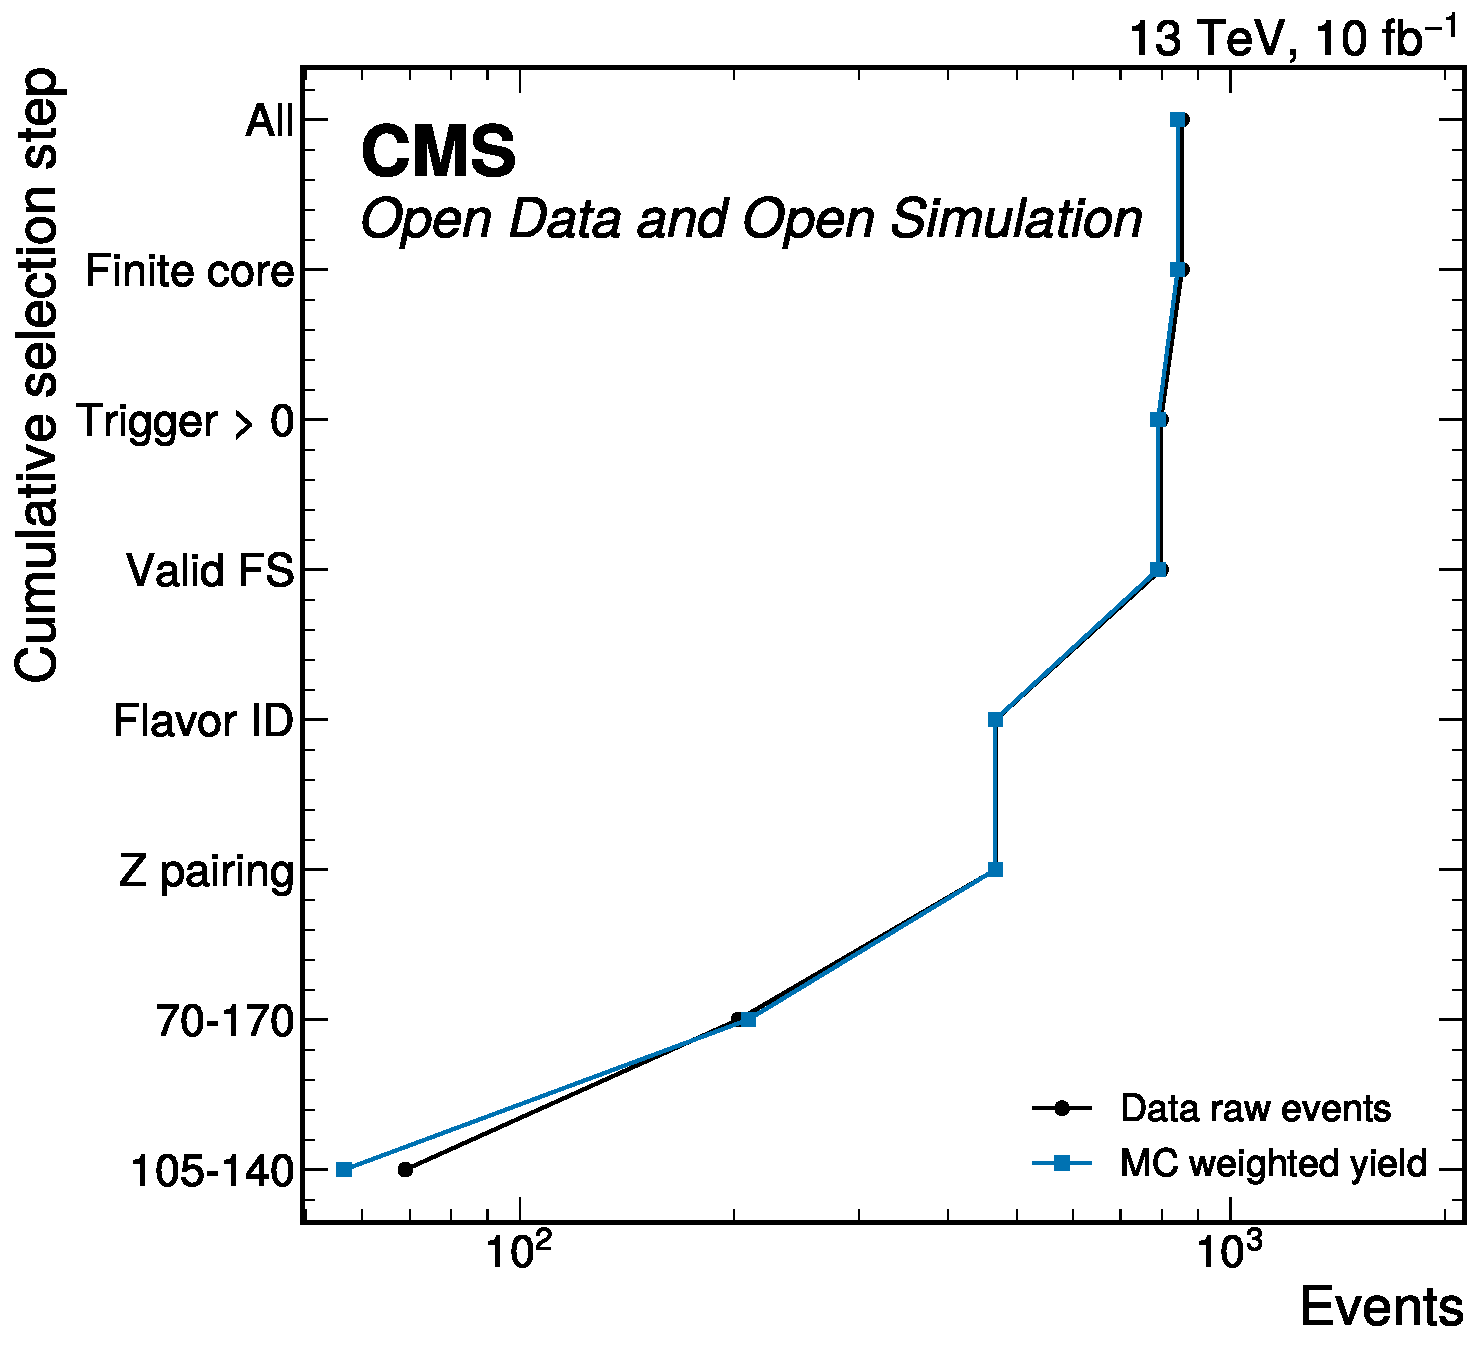
\includegraphics[width=0.92\linewidth,height=0.70\textheight,keepaspectratio]{figures/cutflow_summary.pdf}
\caption{Cumulative Phase 3 cutflow for data raw counts and prompt-normalized MC weighted yields. The rendered step labels are abbreviated for readability; 70--170 GeV is the active signal-strength fit window used by the current Phase 3 handoff and Phase 4 expected, partial, and observed results.}
\label{fig:cutflow-summary}
\end{figure}

\begin{figure}[p]
\centering
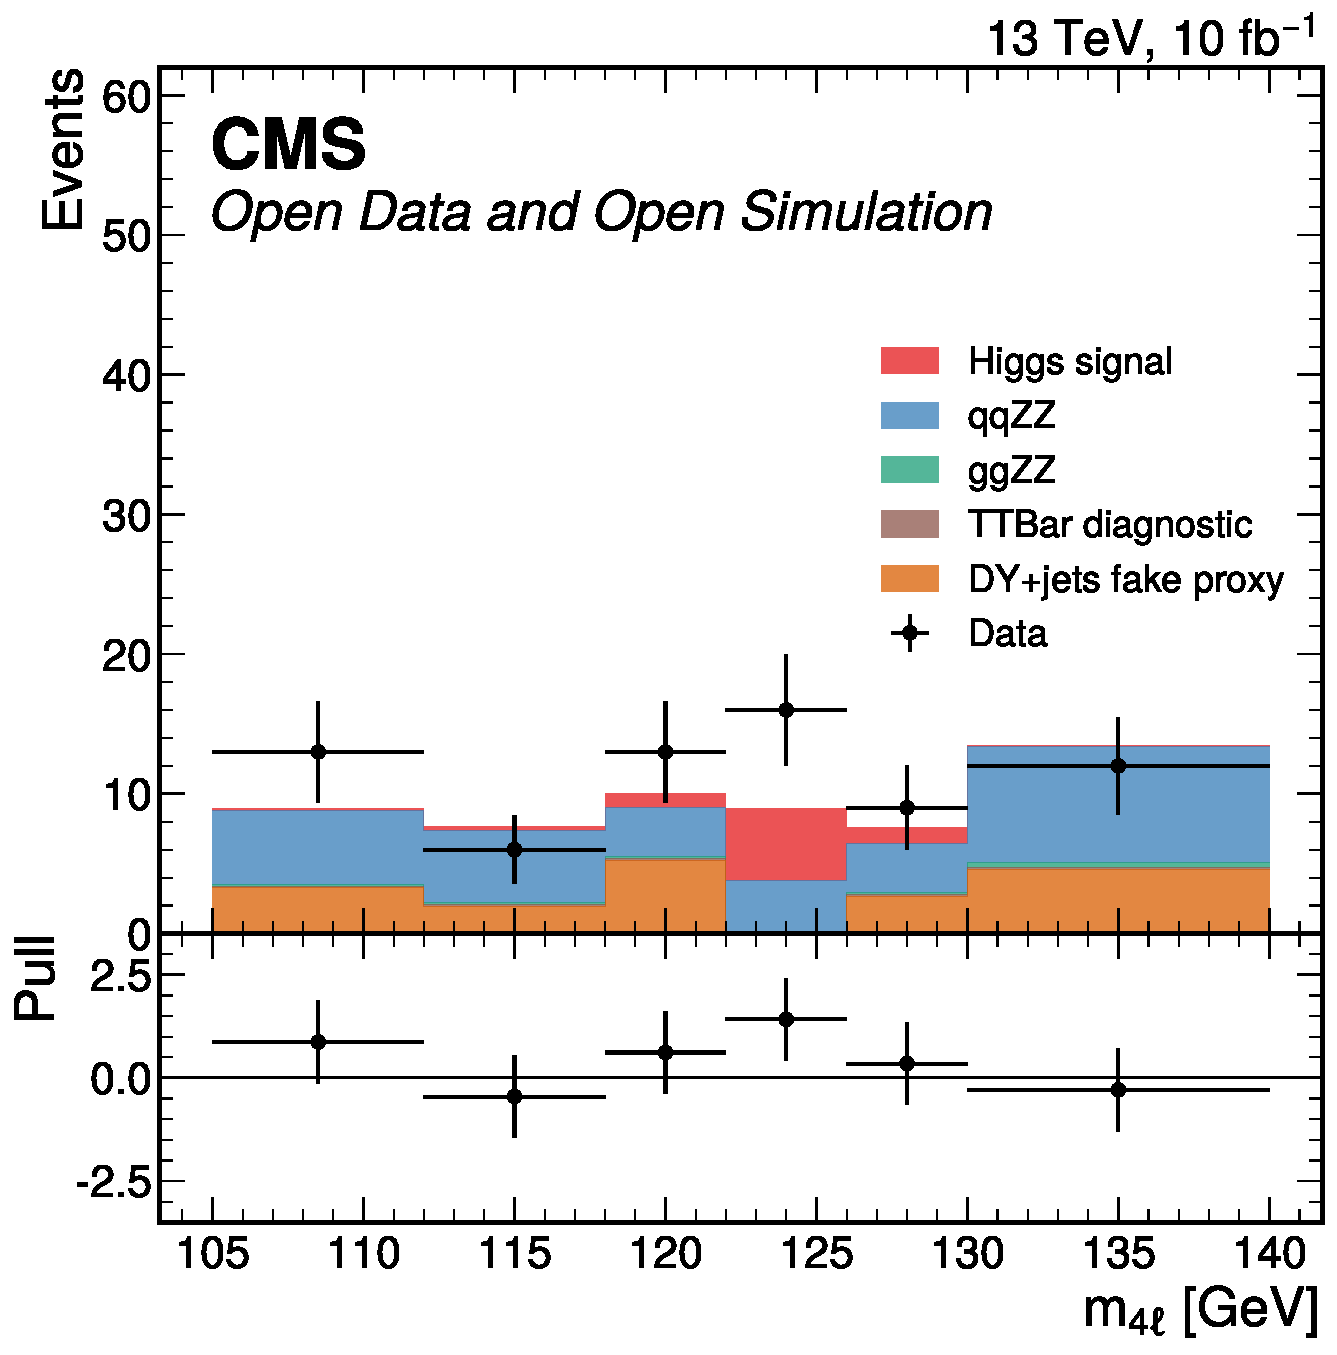
\includegraphics[width=0.92\linewidth,height=0.70\textheight,keepaspectratio]{figures/m4l_fit_window_inclusive.pdf}
\caption{Historical narrow-window inclusive four-lepton mass diagnostic retained from Phase 3. The current signal-strength results use the broad 70--170 GeV template figures; this plot is preserved only as auxiliary selection context, not as the active fit-window definition.}
\label{fig:m4l-fit-window-inclusive}
\end{figure}

\begin{figure}[p]
\centering
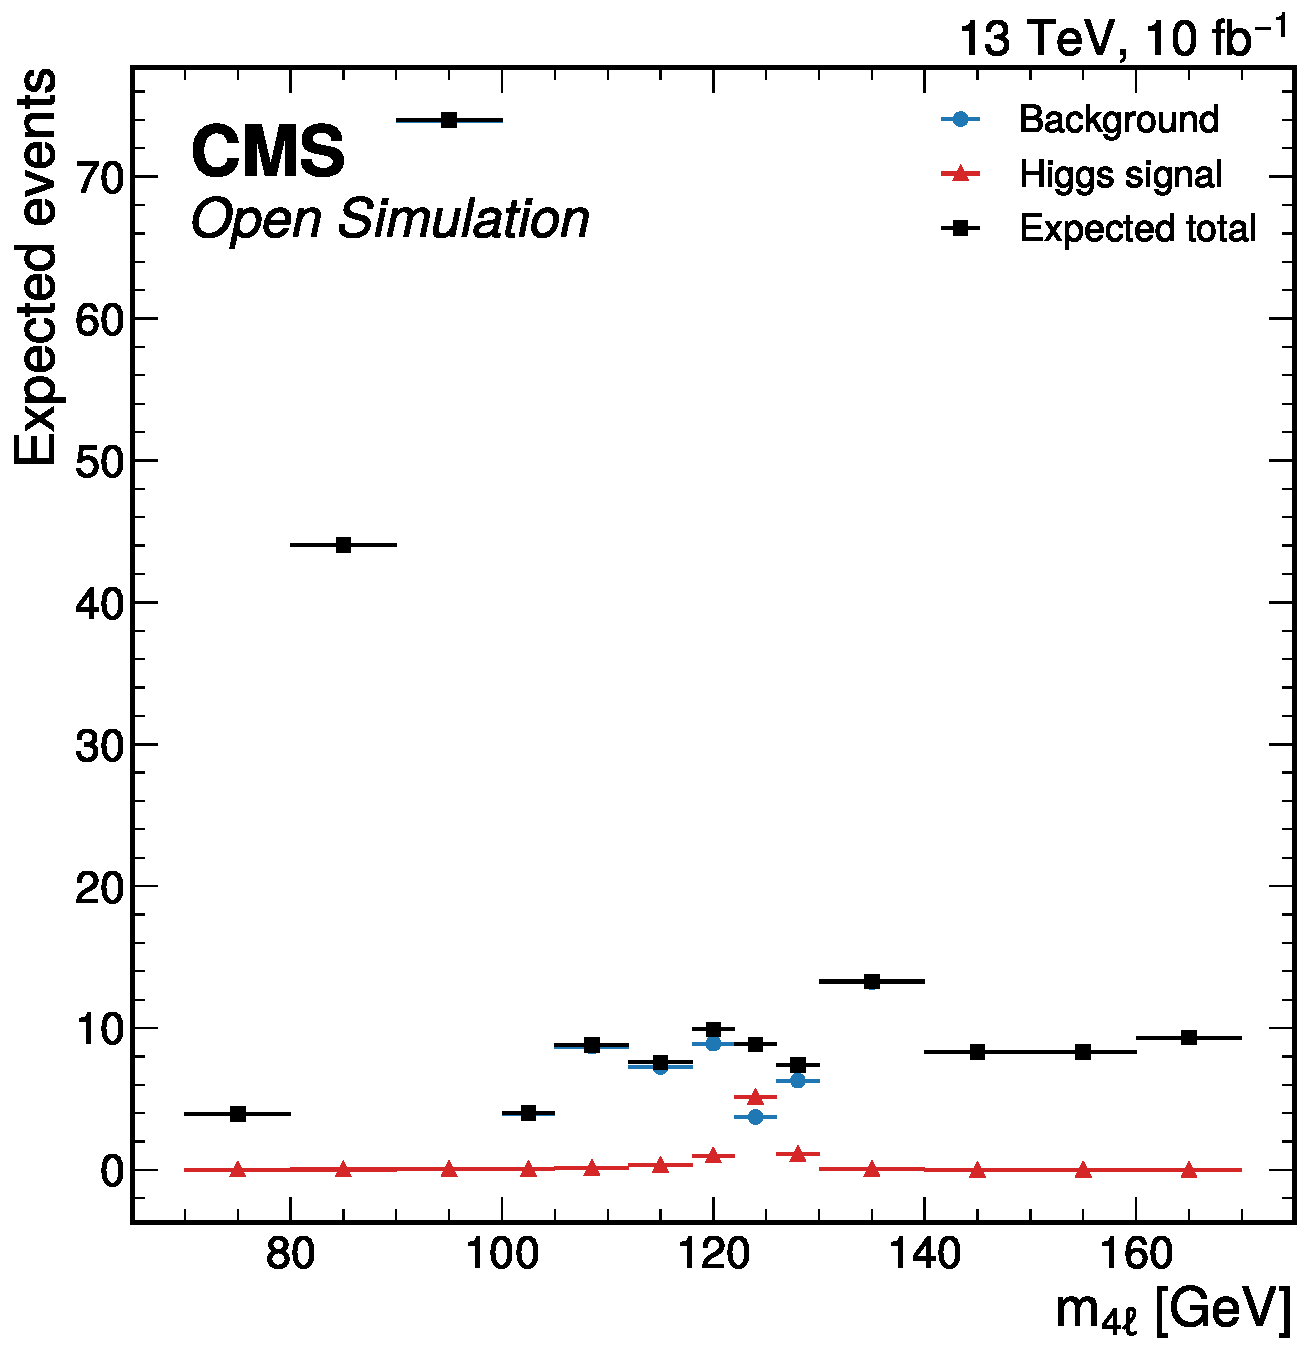
\includegraphics[width=0.92\linewidth,height=0.70\textheight,keepaspectratio]{figures/expected_m4l_broad_inclusive.pdf}
\caption{Expected inclusive four-lepton mass distribution in the broad validation range 70 < m4l < 170 GeV. The broad display is the current Phase 4a expected signal-strength template range and matches the Phase 4b/4c observed fit window, including the Z peak.}
\label{fig:expected-m4l-broad-inclusive}
\end{figure}

\begin{figure}[p]
\centering
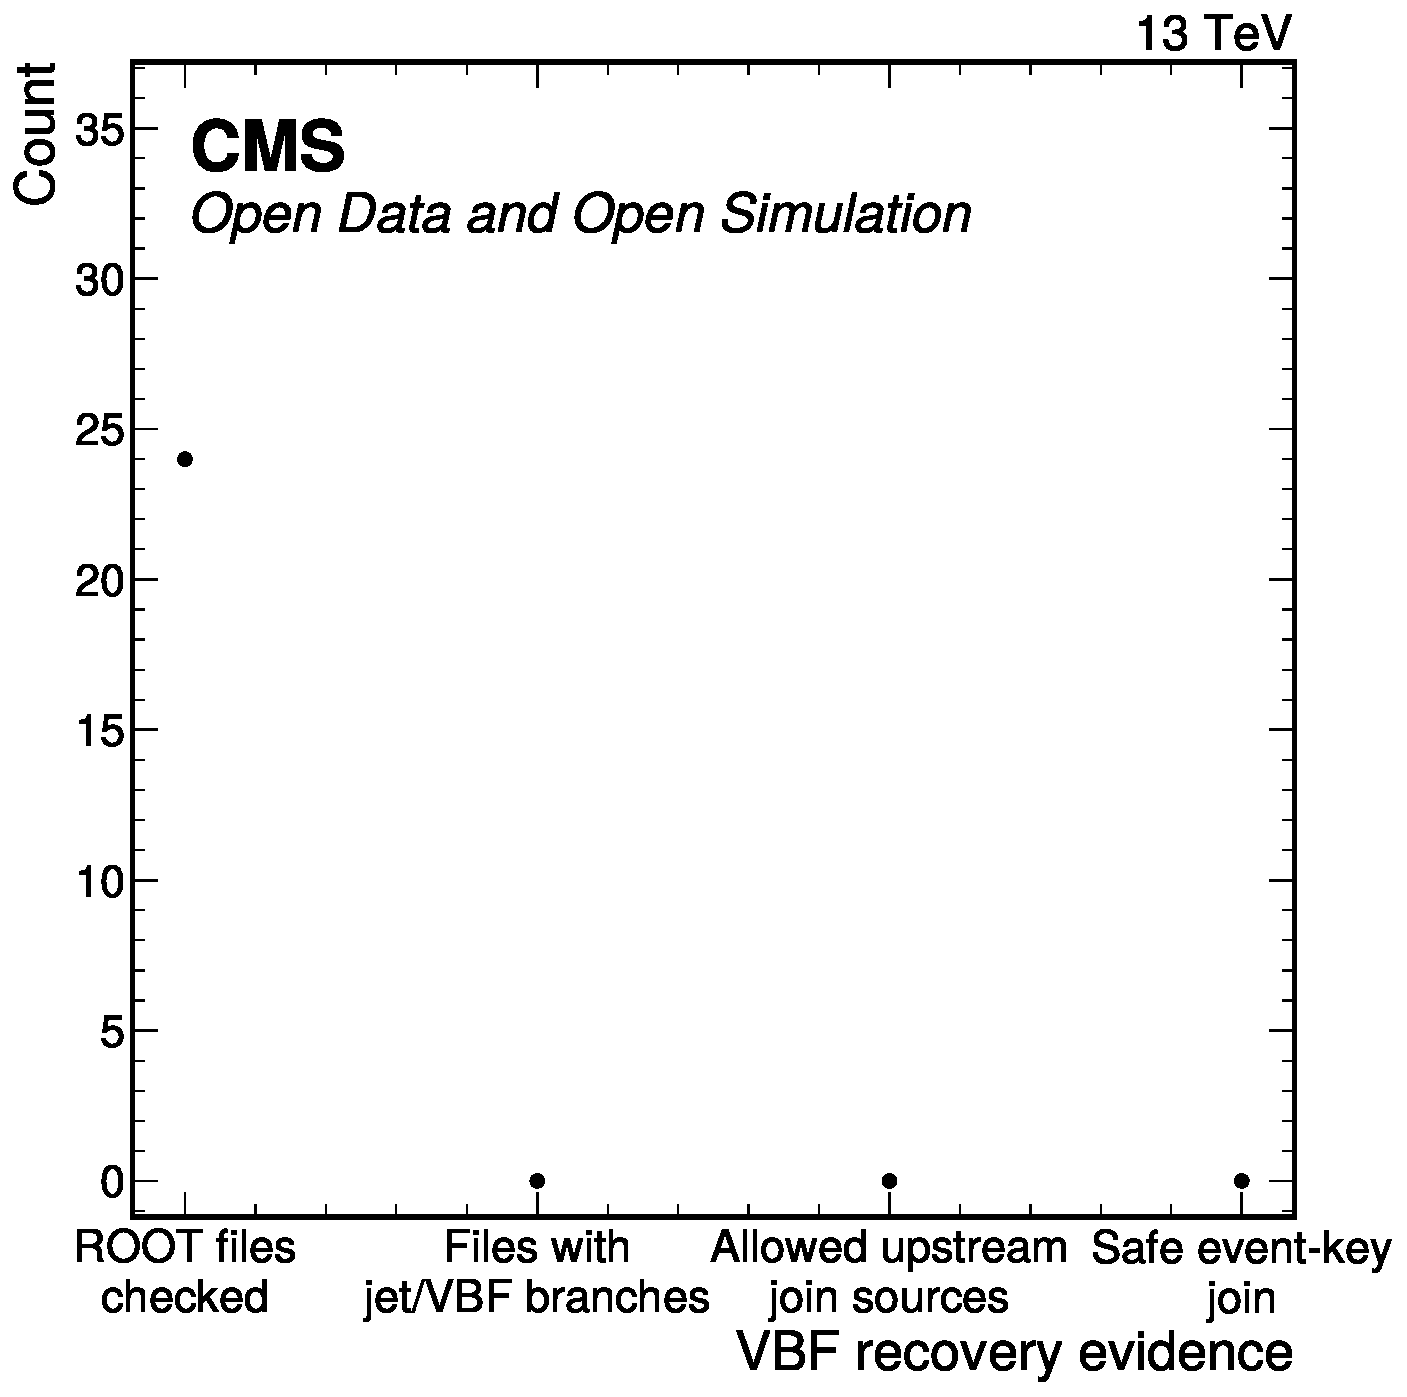
\includegraphics[width=0.92\linewidth,height=0.70\textheight,keepaspectratio]{figures/vbf_downscope_evidence.pdf}
\caption{VBF recovery and downscope evidence from branch inventories and allowed join sources. No checked flat ntuple contains real jet or VBF discriminator branches, no allowed upstream join source exists, and no lepton-only category is labeled VBF.}
\label{fig:vbf-downscope-evidence}
\end{figure}

\begin{figure}[p]
\centering
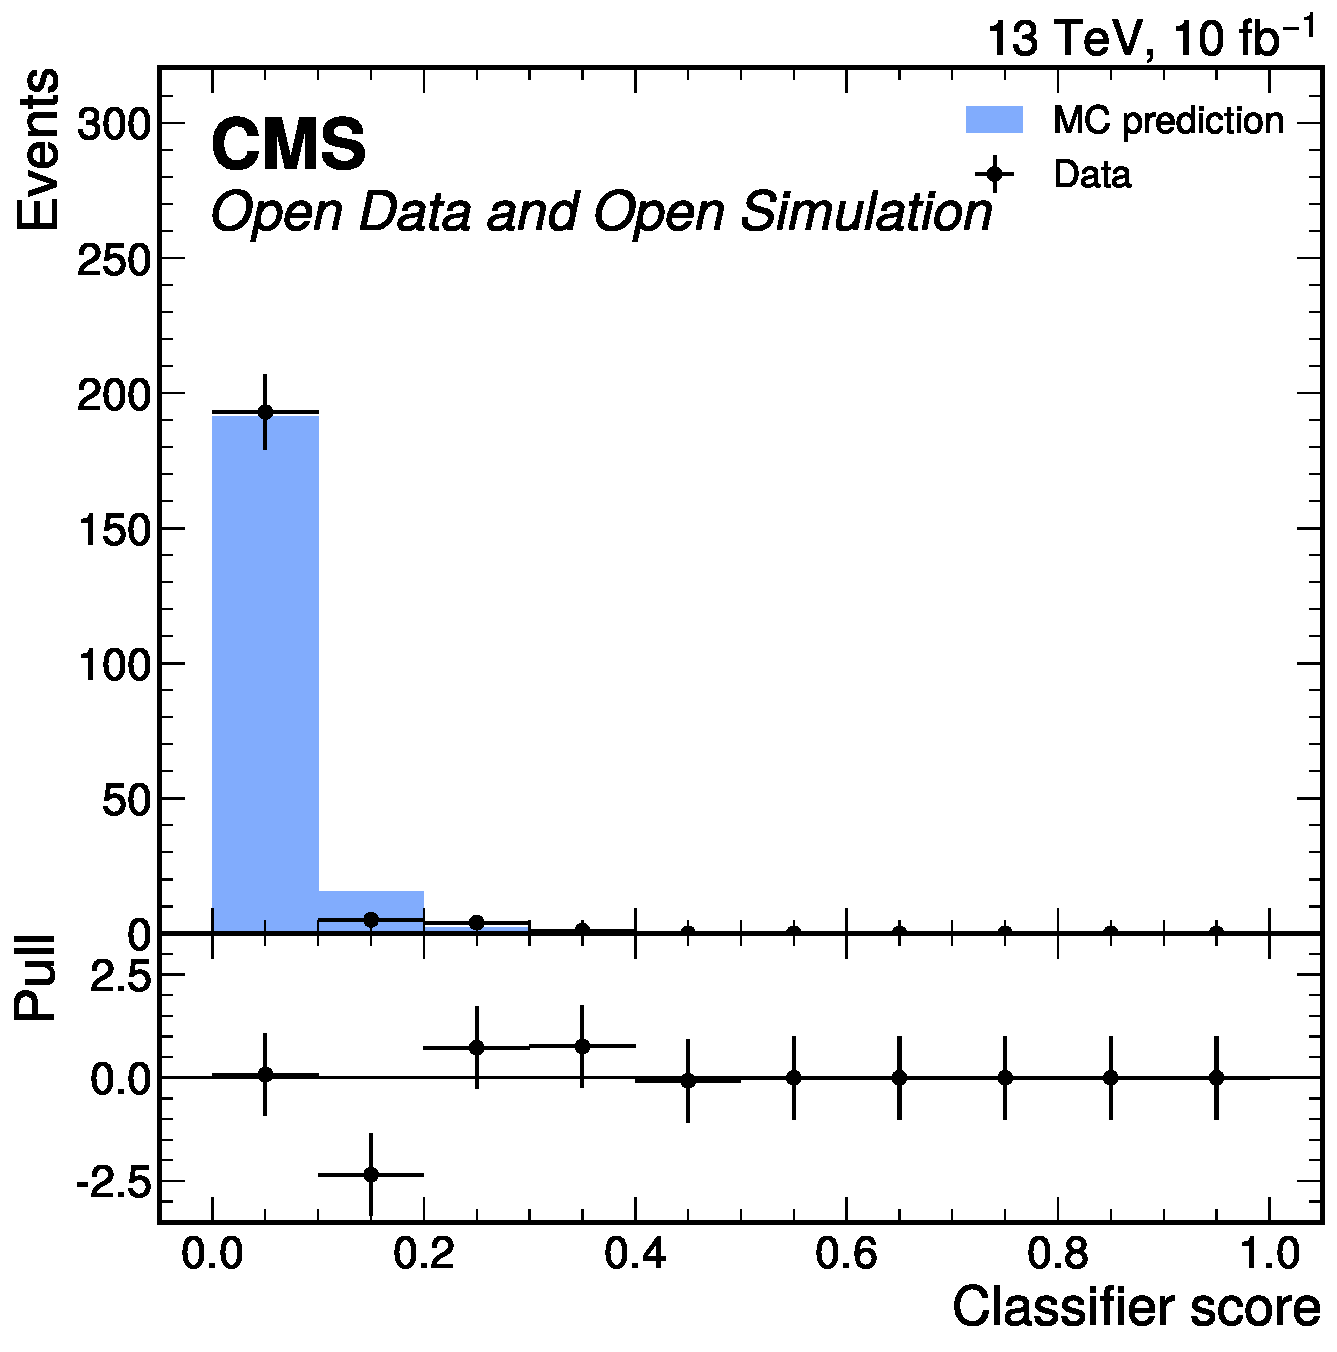
\includegraphics[width=0.92\linewidth,height=0.70\textheight,keepaspectratio]{figures/mva_best_score_datamc.pdf}
\caption{Best S2 classifier score data/MC comparison in the broad validation window. The score-shape gate and low-stat category viability failed, so this diagnostic is preserved as rejected-approach evidence rather than used in the nominal fit.}
\label{fig:mva-best-score-datamc}
\end{figure}

\begin{longtable}{lllll}
\caption{Input-variable modeling gate for classifier attempts. Only variables passing all D7 requirements were eligible, and the final classifier categories still failed promotion.}\label{tab:input-gate}\\
\toprule
Variable & $\chi^2$/ndf & p-value & max ratio dev. & D7 pass \\ 
\midrule
\endfirsthead
\toprule
Variable & $\chi^2$/ndf & p-value & max ratio dev. & D7 pass \\ 
\midrule
\endhead
cos\_theta1 & 1.6 & 0.1562 & 0.5568 & no \\
cos\_theta2 & 1.289 & 0.2655 & 0.4591 & no \\
cos\_theta\_star & 1.007 & 0.4115 & 0.3637 & no \\
eta4l & 0.4039 & 0.8464 & 0.2204 & no \\
lead\_abs\_eta & 0.4734 & 0.7553 & 0.1931 & yes \\
lead\_lepton\_pt & 4.056 & 0.002731 & 1 & no \\
mZ1 & 122.1 & 6.22e-155 & 1 & no \\
mZ2 & 32.08 & 7.49e-39 & 1 & no \\
phi & 0.7802 & 0.5637 & 0.2509 & no \\
phi1 & 0.1552 & 0.9785 & 0.08262 & yes \\
pt4l & 0.3328 & 0.8934 & 0.3478 & no \\
sublead\_abs\_eta & 1.076 & 0.3664 & 0.2433 & no \\
sublead\_lepton\_pt & 849.5 & 0 & 1 & no \\
y4l & 996.7 & 0 & 1 & no \\
\bottomrule
\end{longtable}


\section{Corrections and Model Construction}
This measurement is detector-level. There is no particle-level unfolding because the flat ntuples do not retain generator-level truth branches or a response matrix. The relevant correction step is MC normalization and template construction: selected MC events are weighted with Eq.~\ref{eq:mc-weight}, grouped into signal and background templates, and binned in $m_{4\ell}$ by final-state category.

The expected bin content for process group $g$, category $c$, and mass bin $b$ is
\begin{equation}
 \nu_{gcb}(\boldsymbol{\theta}) = \sum_{s\in g}\sum_{i\in(s,c,b)} w_s\,a_{gcb}(\boldsymbol{\theta}),
 \label{eq:template-content}
\end{equation}
where $a_{gcb}(\boldsymbol{\theta})$ is the nuisance-dependent rate or shape modifier. The total expected content is
\begin{equation}
 \lambda_{cb}(\mu,\boldsymbol{\theta}) = \mu\sum_{g\in H}\nu_{gcb}(\boldsymbol{\theta}) + \sum_{g\in B}\nu_{gcb}(\boldsymbol{\theta}).
 \label{eq:expected-content}
\end{equation}
The Phase 4a observation is Asimov pseudo-data equal to the nominal expectation; Doc 4b and Doc 4c then fit observed Open Data subsamples with the same broad-window template structure.

Shape and rate variations are propagated by producing up/down shifted templates. For a rate-only systematic with relative size $\delta_k$, the variation is
\begin{equation}
 \nu^{\pm}_{gcb,k}=\nu^{0}_{gcb}(1\pm\delta_k),
 \label{eq:rate-syst}
\end{equation}
while the $m_{4\ell}$ scale systematic is implemented as a histosys-like shifted-template variation. The grouped MC-stat approximation uses process/category normalization nuisances derived from Phase 3 sum of squared weights:
\begin{equation}
 \delta^{\mathrm{MCstat}}_{gc}=\frac{\sqrt{\sum_b \mathrm{sumw2}_{gcb}}}{\sum_b \nu_{gcb}}.
 \label{eq:mcstat-grouped}
\end{equation}
This is formally downscoped relative to full per-bin HistFactory staterror profiling \cite{HistFactory}; alternative-binning stability is used to check that it does not dominate the expected conclusion.

The template construction keeps two normalizations separate. Shape-comparison plots used during input validation may rescale MC to the data integral to expose mismodeling in candidate classifier variables, but those diagnostic scales never enter Eq.~\ref{eq:template-content}. Fit templates use only the luminosity and prompt-effective cross-section weights in Eq.~\ref{eq:mc-weight}. This separation is important because otherwise the signal-strength fit would become partly circular: a background or signal normalization inferred from observed data in the signal window would reduce the very rate information used to estimate $\mu$.

The nominal grouping also preserves the distinction between physics components even when they are added in the final likelihood. The Higgs signal group contains ggH, VBF, WH, WplusH, WminusH, and ZH templates; the single POI multiplies their sum. The irreducible background is split into qqZZ and ggZZ groups because they have different production mechanisms and nuisance sizes. The reducible background remains DY+jets, with TTBar retained only as an omission diagnostic. This grouping is the minimum structure needed to compare to CMS H to four-lepton analyses without claiming production-mode measurements that the available categories cannot support.

The downscope decisions enter the model construction directly. Since no VBF category is recoverable, VBF events contribute only to the inclusive signal template and no jet-energy or VBF-migration nuisance is created. Since the classifier categories are rejected, angular variables and MVA scores do not partition the likelihood. Since no particle-level response exists, the result is not unfolded and no acceptance correction is applied. These absences are encoded in the systematic-source table rather than hidden in prose.

The correction/model section is intentionally explicit because it replaces an unfolding section for this detector-level analysis. The procedure is reproducible from the sample inventory, selection definitions, binning, and JSON template payloads. It also defines the main limitation: the reported $\mu$ is a signal-strength fit relative to the prompt-effective MC expectation and not a fiducial cross-section extraction with independent acceptance, branching-fraction, or particle-level corrections.
\section{Systematic Uncertainties}
The systematic model follows the reviewed Phase 4a expected workspace. Active sources are propagated as normalization or shape modifiers in the binned likelihood; downscoped or inapplicable sources are still documented because they affect interpretation and comparison to CMS reference analyses.

The covariance decomposition for the single POI is
\begin{equation}
 V_{\mathrm{tot}} = V_{\mathrm{stat}} + V_{\mathrm{syst}},
 \label{eq:cov-sum}
\end{equation}
with $V_{\mathrm{stat}}=0.3063689401723719$, $V_{\mathrm{syst}}=0.023955108369782596$, and $V_{\mathrm{tot}}=0.33032404854215447$ for $\mu$. The MC-stat component inside the systematic budget contributes variance 0.0029560843175981955.

\begin{small}
\begin{longtable}{p{0.08\linewidth}p{0.18\linewidth}p{0.25\linewidth}p{0.13\linewidth}p{0.20\linewidth}}
\caption{Systematic source inventory from systematics\_sources.json.}\label{tab:syst-sources}\\
\toprule
Label & Key & Source & Size & Status \\ 
\midrule
\endfirsthead
\toprule
Label & Key & Source & Size & Status \\ 
\midrule
\endhead
SP1 & lumi & Integrated luminosity & 0.008072 & implemented \\
SP4 & lepton eff & Lepton reco/ID/trigger & 0.03 & implemented \\
SP7 & signal theory & Signal production & 0.05 & fallback prior \\
SP9 & ZZ norm & qqZZ background normalization & 0.1 & fallback prior \\
SP9 & ggZZ norm & ggZZ background normalization & 0.2 & fallback prior \\
SP10 & DY norm & DY+jets fake proxy & 0.5 & implemented \\
SP11 & ttbar omission & TTBar omission diagnostic & 0.0444 & implemented \\
SP5 & m4l scale & Lepton m4l scale & 0.001 & implemented \\
SP3 & mc stat & MC statistical uncertainty & n/a & grouped MC-stat downscope \\
SP2 & prompt xsecs & Prompt xsecs & per-sample prompt xsecs & implemented prompt fallback \\
SP6 & pileup/PV & Pileup/PV & n/a & not propagated \\
SP8 & Higgs BR & Higgs BR & n/a & not applicable \\
SP12 & classifier & Classifier migration & n/a & not applicable \\
SP13 & angular & Angular reco & n/a & not propagated \\
\bottomrule
\end{longtable}
\end{small}

\subsection{Integrated Luminosity}
Integrated luminosity changes the normalization of all simulated templates. It is evaluated as a log-normal normalization nuisance using the public CMS 2017 luminosity uncertainty as a scale reference for the user-provided 10 fb$^{-1}$ subset. The relative variation is 0.008072174738841406, producing a small expected impact on $\mu$ because the fit uncertainty is dominated by statistical power and background modeling. This source would become more important in an observed cross-section extraction, but in Phase 4a it is propagated only as a rate uncertainty.

\subsection{Prompt Effective Cross Sections}
Prompt cross sections define nominal MC weights and are not independently tuned to data. Phase 4a mitigates this by carrying process normalization nuisances for signal and background groups and by recording the prompt source trail. The result should be interpreted as a signal strength relative to these prompt-effective sample normalizations, not as a standalone fiducial cross section.

\subsection{MC Statistical Uncertainty}
MC statistical uncertainty is propagated through grouped process/category normalization nuisances derived from Phase 3 sumw2. This is a formal downscope from full bin-by-bin HistFactory staterror profiling, which was not computationally stable in the sandbox. The grouped component contributes variance 0.0029560843175981955 and is checked through alternative binnings. Downstream observed-data phases must repeat the stability checks.

\subsection{Lepton Efficiency}
Lepton reconstruction, identification, and trigger efficiency affect every signal and background template because all selected objects are electrons or muons. The Phase 4a implementation uses a 0.03 rate envelope derived from Phase 3 trigger and flavor-matched ID data/MC step-efficiency closure. This is a detector-level envelope rather than an official CMS scale-factor chain. The expected $\mu$ impact is visible in the nuisance impact table and is subdominant to DY fake-proxy and ZZ normalization uncertainties.

\subsection{Lepton Momentum Scale and Resolution}
Lepton momentum scale and resolution influence the reconstructed four-lepton mass shape. Phase 4a propagates this as an $m_{4\ell}$ template shift corresponding to a 0.001 variation. This is not an official CMS lepton calibration; it is an external performance-envelope approximation applied to the available detector-level templates. The low-count corruption sensitivity study shows that a -20\% mass-response corruption is not rejected in the final-state workspace, so this source is also tied to a documented sensitivity limitation.

\subsection{Pileup and Primary Vertex Modeling}
Pileup and primary-vertex modeling are documented but not propagated because PV variables are not used in the nominal selection categories or fit templates. Phase 3 excluded pvNdof and related variables under the validation gate. This is an explicit not-propagated status, not a silent omission.

\subsection{Signal Production Composition}
Signal production and composition uncertainty accounts for the relative mixture of ggH, VBF, WH, WminusH, WplusH, and ZH signal templates. The flat ntuples do not provide all official generator-composition inputs, so Phase 4a uses a 0.05 fallback prior and marks it as an expected-phase approximation. It is propagated separately over signal production groups while one global $\mu$ scales the total Higgs yield. Because no VBF category is available, this source mostly changes the inclusive signal normalization rather than category migration.

\subsection{Higgs Branching Fraction}
The Higgs BR is not used in Phase 4a because no fiducial or inclusive cross-section conversion is performed. The reported quantity is detector-level $\mu$ relative to the nominal Higgs MC templates. If a later phase converts to a cross section, the branching-fraction source must be activated and cited.

\subsection{qqZZ Background Normalization}
The dominant irreducible continuum background is qqZZ. Its normalization is varied by 0.1 as a fallback prior due to unavailable campaign-specific validation of the prompt effective cross section. The variation is applied to the background ZZ template in all final states. It is one of the largest systematic variance components, which is expected because the signal region contains substantial ZZ continuum under the Higgs peak.

\subsection{ggZZ Background Normalization}
The loop-induced ggZZ background is represented by the three GGZZ final-state samples. A 0.2 fallback normalization prior is used because the small effective cross sections and prompt-provided sample definitions cannot be independently validated to official precision in this sandbox. Its expected impact on $\mu$ is small compared with qqZZ and DY because the selected ggZZ yield is small.

\subsection{DY plus Jets Fake Proxy}
DY+jets is the nominal reducible fake-background proxy by user instruction. The official CMS analyses use data-driven Z+X estimates, so this source is a comparability limitation. Phase 4a assigns a 0.5 normalization variation based on low sideband statistics and fake-model limitations. It is the largest single nuisance impact on expected $\mu$, which correctly reflects the weak constraint provided by the available DY selected sample.

\subsection{TTBar Omission Diagnostic}
TTBar is not promoted to a nominal separate fake component because its weighted yield is below the Phase 2 thresholds relative to DY+jets in the signal and sideband windows. The omission diagnostic is retained as a 0.0444 envelope on the reducible background. Its numerical impact is small, but documenting it prevents the DY-only fake proxy from being interpreted as a complete reducible-background estimate.

\subsection{Classifier Migration}
Classifier migration uncertainty is not applicable in the nominal fit because S2 classifier categories, including the neural-network attempt, were rejected. The diagnostics are retained in the appendix to show why the route was not promoted. If a later phase revisits classifier categories, this source must be reactivated with score-boundary migration variations.

\subsection{Angular Reconstruction}
Angular reco passed closure, with median mass differences far below 0.1 GeV and no out-of-range angles in checked selected events. It is not propagated as a nominal fit systematic because angular variables are not used after S2 rejection. The closure remains important evidence that the NN attempt was made on physically sensible inputs.

\subsection{VBF and Jet Systematics}
Jet/VBF category systematics are formally downscoped because there is no recoverable jet or VBF information in the allowed ntuples. No VBF category exists in the nominal model, and no lepton-only category is labeled VBF. This makes official VBF-category comparisons unavailable rather than weakly measured.

\begin{table}[htbp]
\centering
\caption{Largest nuisance impacts on expected $\mu$. Shifts are fixed-variation expected impacts, not observed-data pulls.}
\begin{tabular}{llll}
\toprule
Nuisance & Down shift & Up shift & Max impact \\ 
\midrule
dy\_fake\_norm & 0.1427 & -0.06093 & 0.1427 \\
qqZZ\_norm & 0.08392 & -0.08207 & 0.08392 \\
lepton eff & 0.05804 & -0.05382 & 0.05804 \\
m4l scale\_shape & -0.009583 & -0.05273 & 0.05273 \\
signal\_ggH\_theory & 0.0462 & -0.04237 & 0.0462 \\
lumi & 0.01497 & -0.01476 & 0.01497 \\
ggZZ\_norm & 0.004351 & -0.004283 & 0.004351 \\
signal\_VBF\_theory & 0.004308 & -0.004223 & 0.004308 \\
ttbar omission & 0.003187 & -0.002649 & 0.003187 \\
signal\_VH\_theory & 0.001326 & -0.001318 & 0.001326 \\
\bottomrule
\end{tabular}
\label{tab:nuisance-impacts}
\end{table}

\begin{figure}[p]
\centering
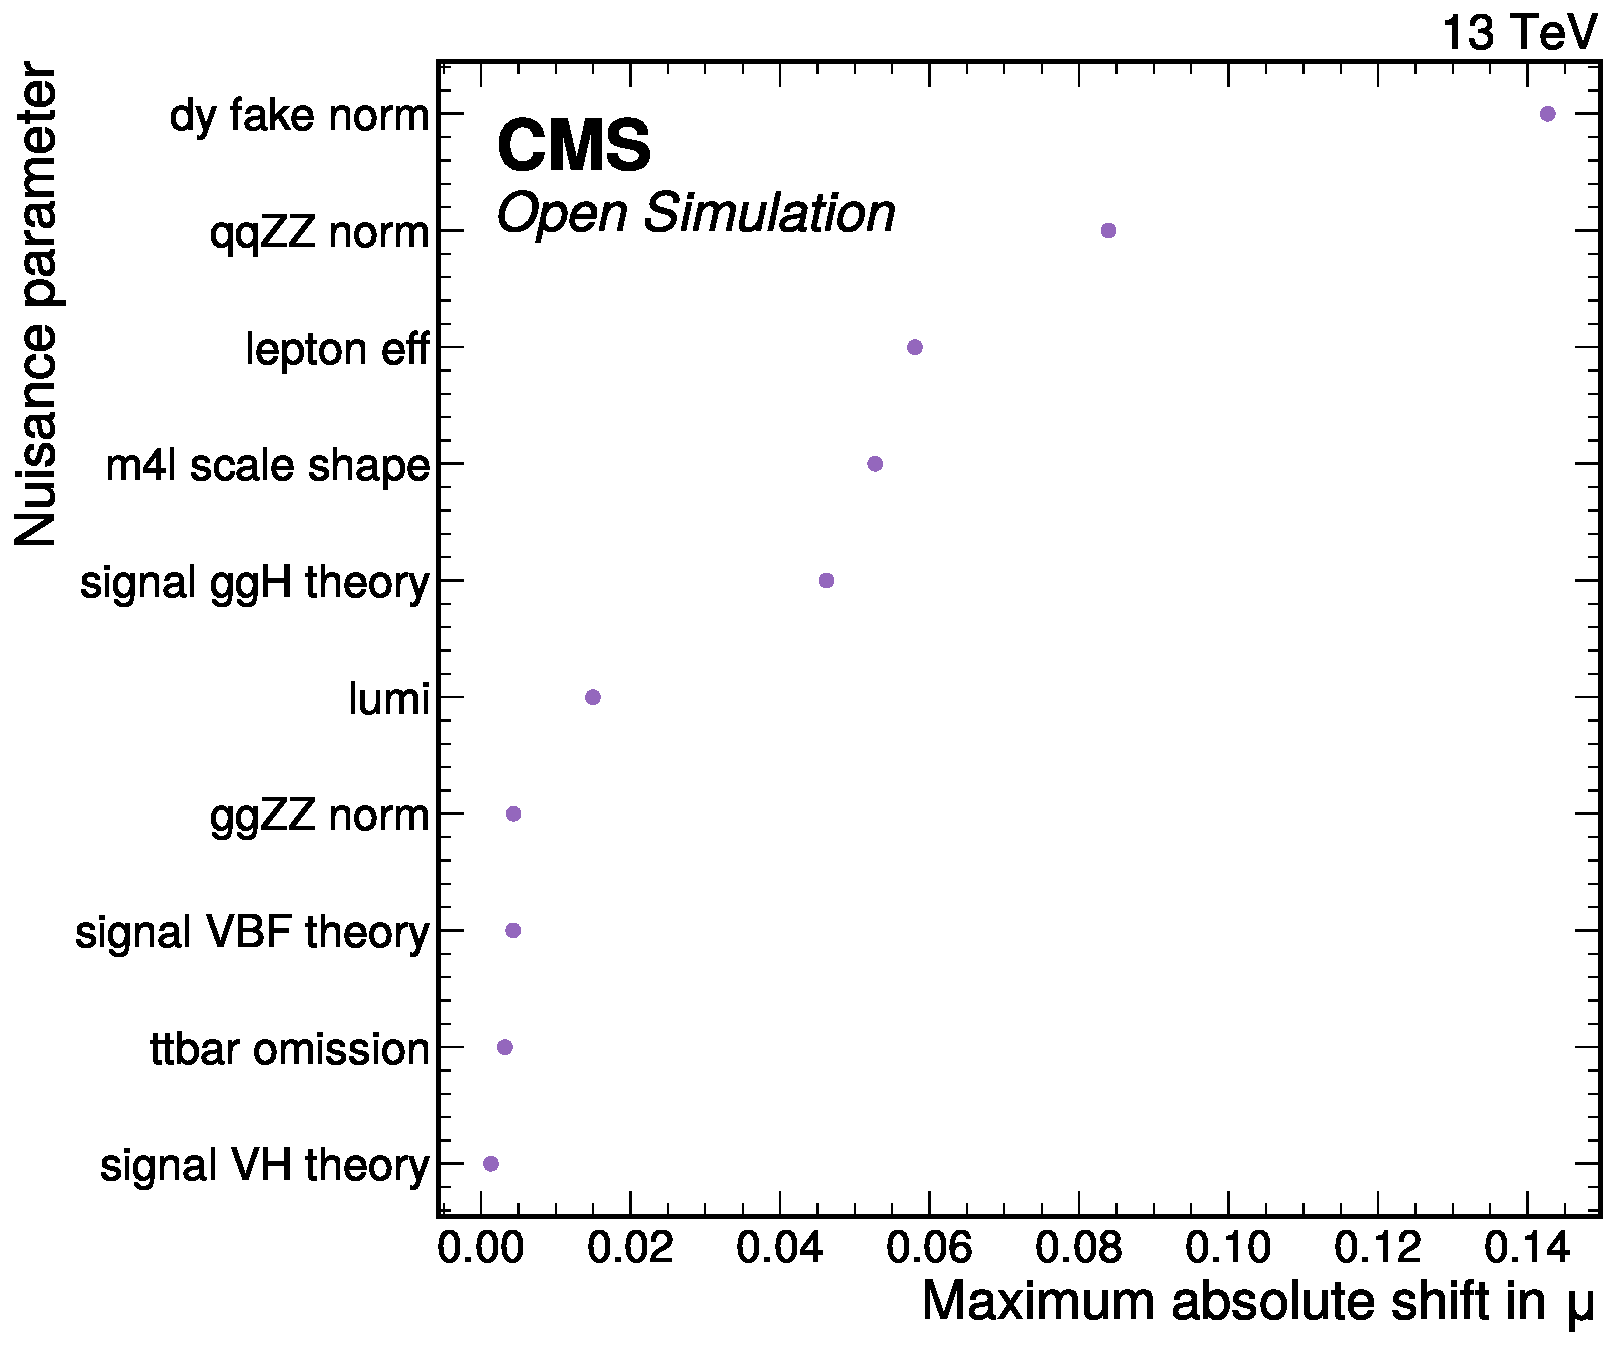
\includegraphics[width=0.92\linewidth,height=0.70\textheight,keepaspectratio]{figures/expected_nuisance_impacts.pdf}
\caption{Expected nuisance impact ranking on the global signal strength, evaluated by fixing each nuisance at plus or minus one standard deviation and refitting the Asimov model.}
\label{fig:expected-nuisance-impacts}
\end{figure}

\begin{figure}[p]
\centering
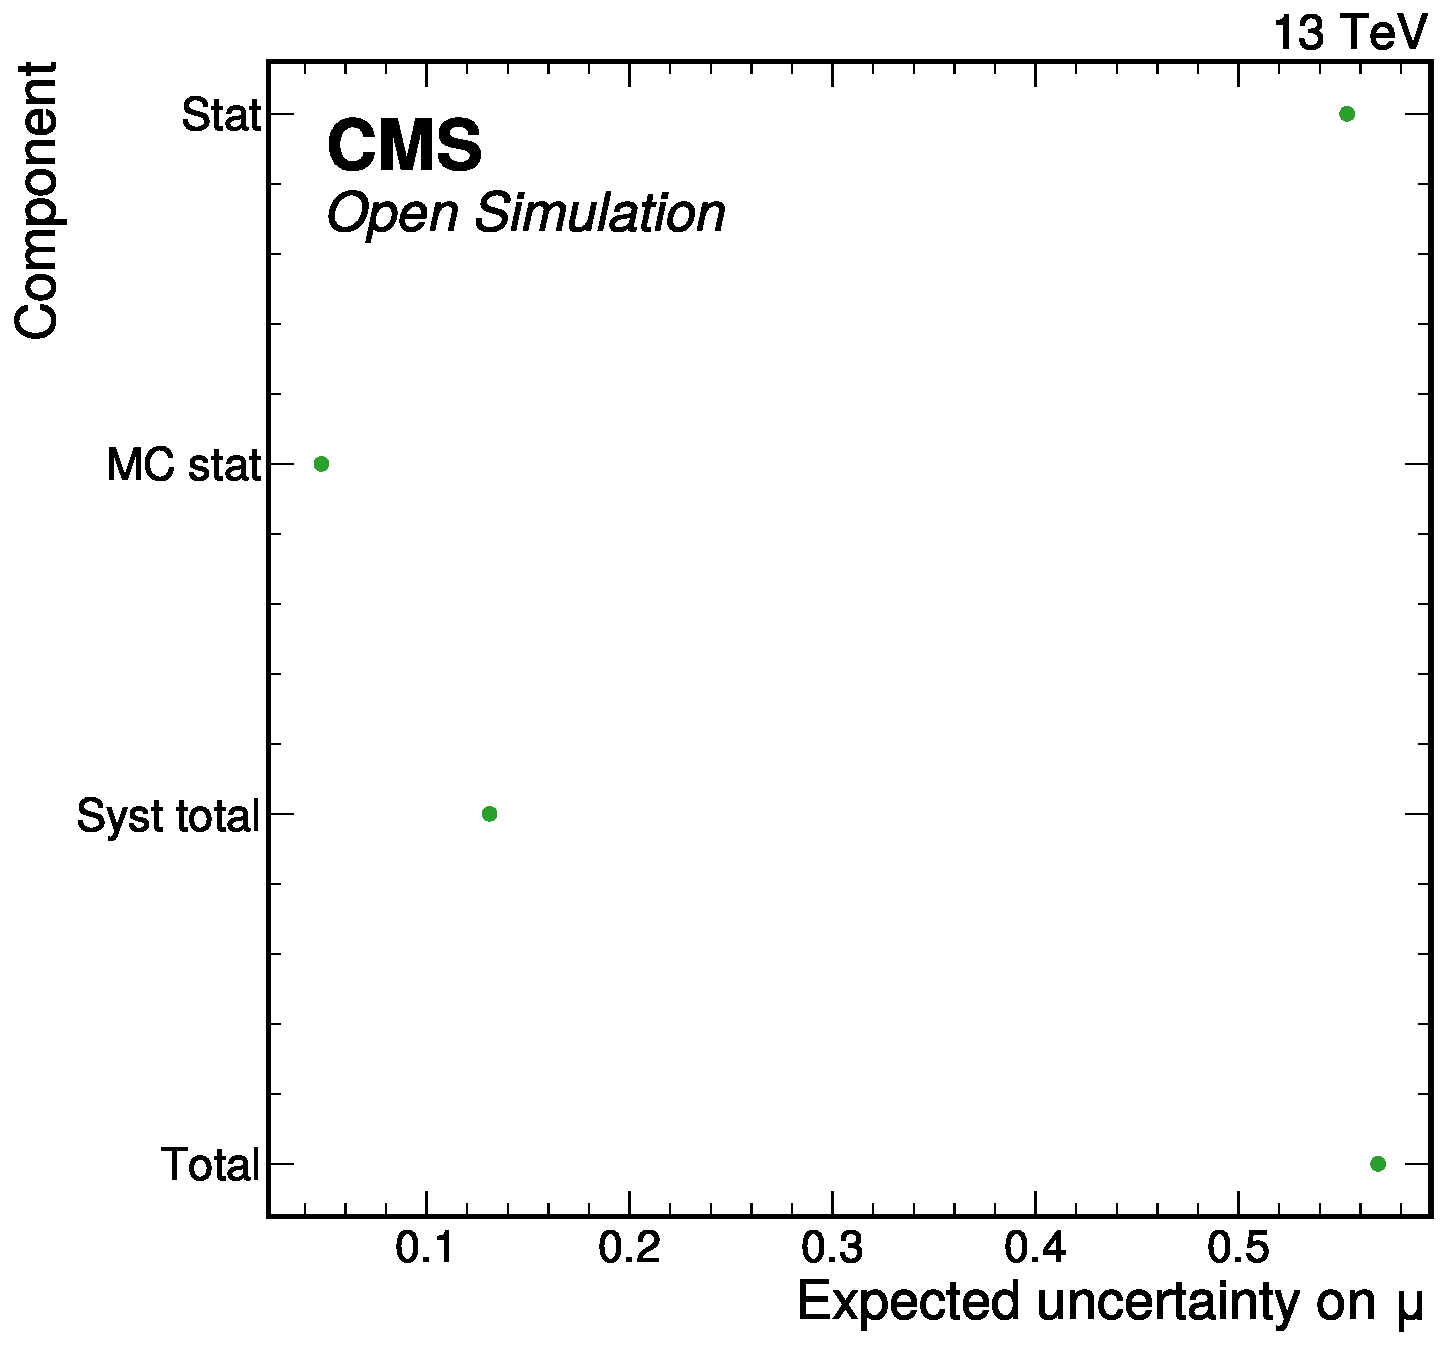
\includegraphics[width=0.92\linewidth,height=0.70\textheight,keepaspectratio]{figures/expected_uncertainty_breakdown.pdf}
\caption{Expected uncertainty breakdown for the Phase 4a Asimov signal-strength fit, derived from the stat-only, MC-stat, and full nuisance fits.}
\label{fig:expected-uncertainty-breakdown}
\end{figure}

\begin{figure}[p]
\centering
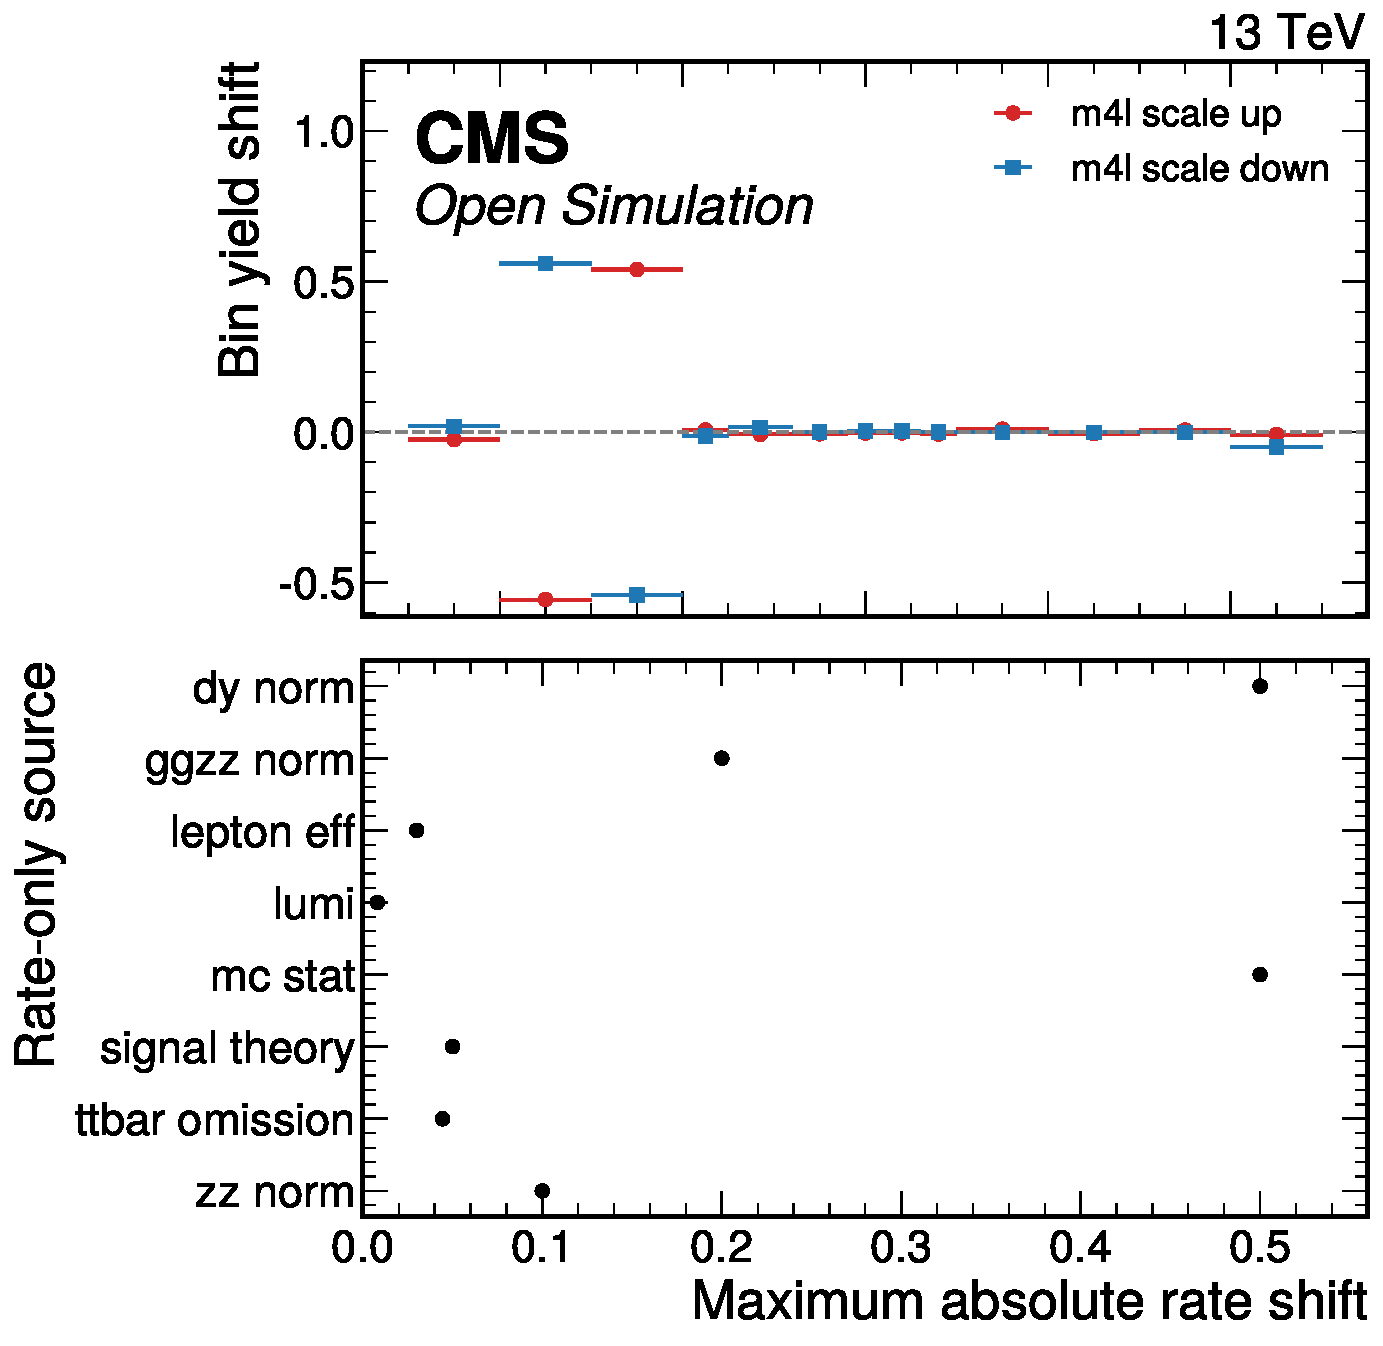
\includegraphics[width=0.92\linewidth,height=0.70\textheight,keepaspectratio]{figures/expected_systematic_shift_summary.pdf}
\caption{Per-systematic shifted-bin summary. The upper panel shows the actual m4l-scale shape-source bin shifts for one representative process/channel; the lower panel shows maximum integral effects for rate-only sources without inventing fake shape dependence.}
\label{fig:expected-systematic-shift-summary}
\end{figure}


\section{Cross-checks}
The cross-checks answer whether the low-count final-state model can be used honestly for expected, 10\% observed, and full observed results. The Asimov goodness-of-fit is exactly zero by construction and is not treated as independent validation. Independent checks are low-count toys, signal injection and recovery, alternative-binning stability, channel compatibility, deterministic split proxies, nuisance behavior, and corrupted-model sensitivity.

For a comparison vector $\mathbf{d}-\mathbf{m}$ with covariance $C$, the generic validation statistic is
\begin{equation}
 \chi^2=(\mathbf{d}-\mathbf{m})^T C^{-1}(\mathbf{d}-\mathbf{m}).
 \label{eq:chi2}
\end{equation}
For low-count Poisson bins the preferred diagnostic is the saturated-model deviance,
\begin{equation}
 D = 2\sum_b \left[n_b\log\frac{n_b}{\lambda_b} - (n_b-\lambda_b)\right],
 \label{eq:poisson-deviance}
\end{equation}
with the usual zero-count convention. In Doc 4c the primary observed GoF is no longer tautological: $\chi^2/\mathrm{ndf}=47.326/38$ with $p=0.1427$, and the Poisson deviance is 48.685 with $p=0.1148$.

\begin{table}[htbp]
\centering
\caption{Signal injection and recovery. All injected Asimov configurations pass the 20\% relative-bias gate.}
\begin{tabular}{lllll}
\toprule
Injected $\mu$ & Fitted $\mu$ & Bias & Relative bias & Pass \\
\midrule
0 & 5.39e-21 & 5.39e-21 & 5.39e-21 & yes \\
1 & 1 & 0 & 0 & yes \\
2 & 2 & -4.47e-06 & 2.24e-06 & yes \\
5 & 5 & -7.58e-05 & 1.52e-05 & yes \\
\bottomrule
\end{tabular}
\label{tab:injection}
\end{table}

\begin{table}[htbp]
\centering
\caption{Full-data alternative-binning stability from observed\_validation.json. The nominal final-state model is retained for the full-data result; inclusive alternatives verify that the fitted signal strength is not a sparse-category artifact.}
\begin{tabular}{llllll}
\toprule
Configuration & Channels & $\hat{\mu}$ & $\sigma_\mu$ & zero bins & GoF p-value \\
\midrule
final\_state\_nominal & 4mu, 4e, 2e2mu & 2.477 & 0.7762 & 3 & 0.1427 \\
inclusive\_nominal & inclusive & 2.537 & 0.7808 & 0 & 0.9132 \\
inclusive\_coarse & inclusive & 2.559 & 0.8133 & 0 & 0.7704 \\
inclusive\_peak\_side & inclusive & 2.560 & 0.8137 & 0 & 0.7282 \\
\bottomrule
\end{tabular}
\label{tab:observed-binning}
\end{table}

\begin{table}[htbp]
\centering
\caption{Full-data final-state category compatibility from observed\_validation.json. The maximum absolute pull relative to the combined result is 0.669, so no final state drives an incompatible signal-strength estimate.}
\begin{tabular}{lllll}
\toprule
Channel & Events & $\hat{\mu}$ & $\sigma_\mu$ & GoF p-value \\
\midrule
4mu & 81 & 2.476 & 1.153 & 0.6966 \\
4e & 24 & 1.106 & 1.899 & 0.9787 \\
2e2mu & 98 & 3.100 & 1.281 & 0.7308 \\
\bottomrule
\end{tabular}
\label{tab:observed-category-compatibility}
\end{table}

\begin{table}[htbp]
\centering
\caption{Full-data deterministic half-split proxy from observed\_validation.json. This is not a true CMS run-period split because run-period metadata are unavailable in the Phase 3 event handoff.}
\begin{tabular}{lllll}
\toprule
Split & Events & Lumi [fb$^{-1}$] & $\hat{\mu}$ & GoF p-value \\
\midrule
split\_a & 103 & 5.0 & $2.350\pm1.108$ & 0.1610 \\
split\_b & 100 & 5.0 & $2.612\pm1.064$ & 0.4074 \\
\bottomrule
\end{tabular}
\label{tab:observed-split}
\end{table}

\begin{figure}[p]
\centering
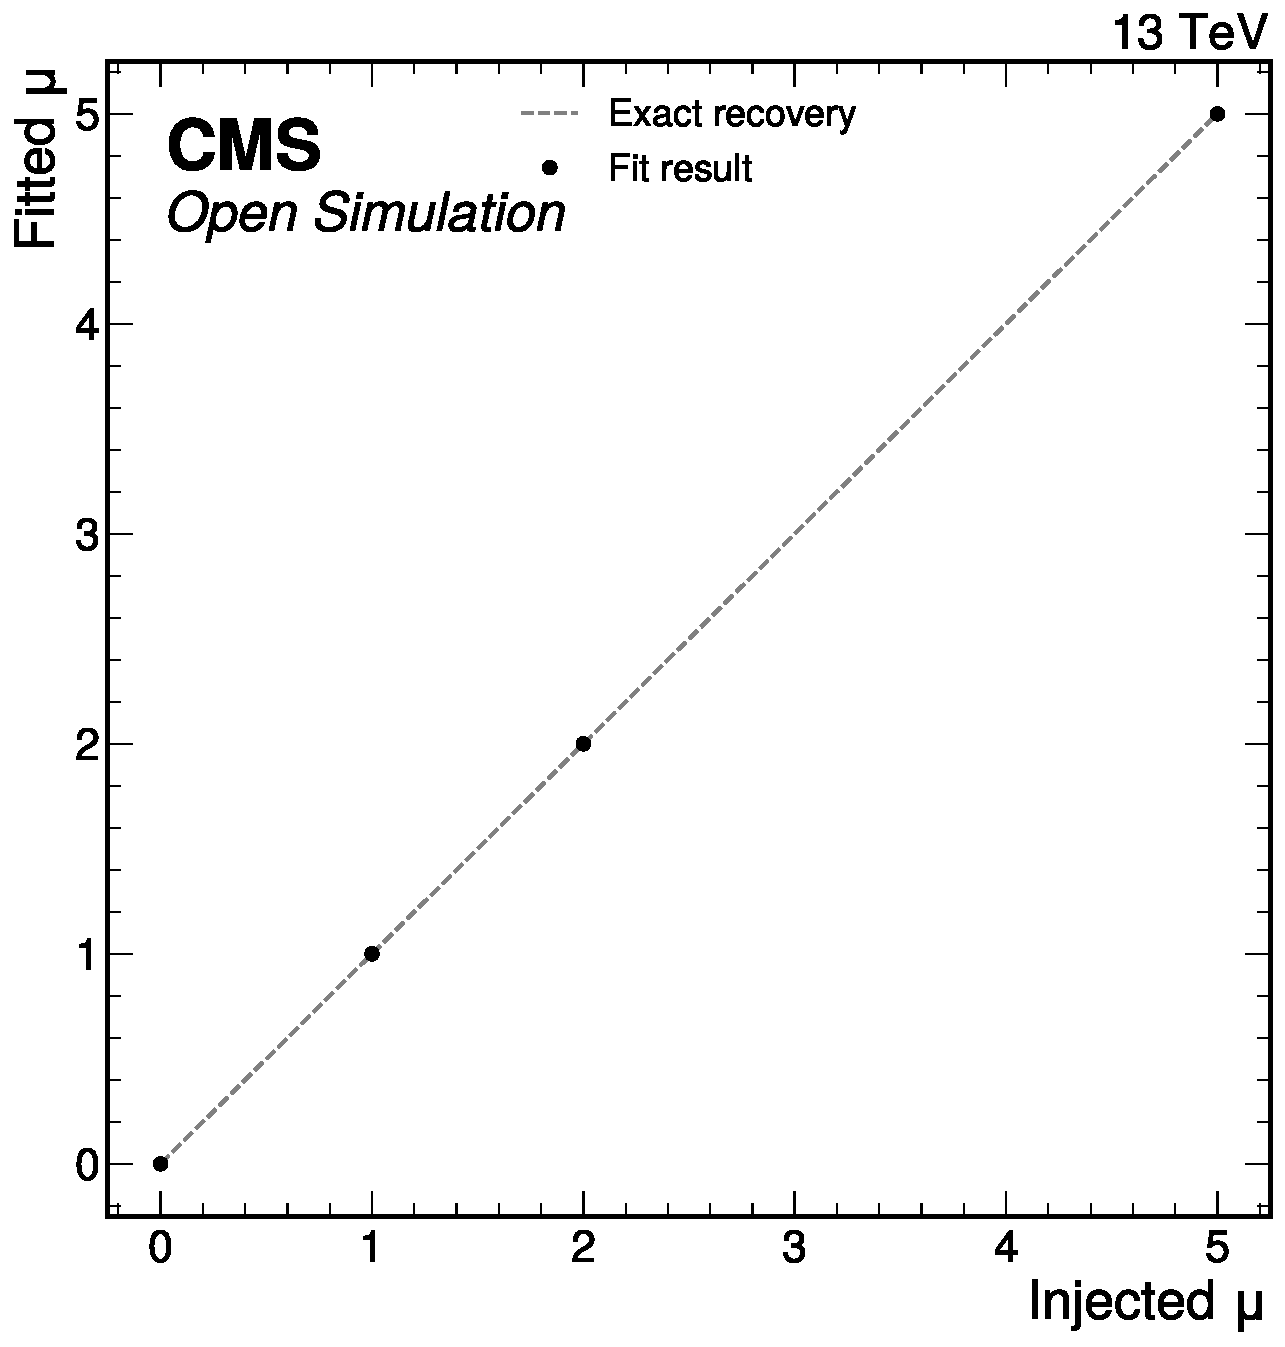
\includegraphics[width=0.92\linewidth,height=0.70\textheight,keepaspectratio]{figures/expected_signal_injection_recovery.pdf}
\caption{Signal injection and recovery test at $\mu = 0$, 1, 2, and 5. All injected Asimov configurations are refit with the same nuisance model and checked against the 20 percent bias gate.}
\label{fig:expected-signal-injection-recovery}
\end{figure}

\begin{figure}[p]
\centering
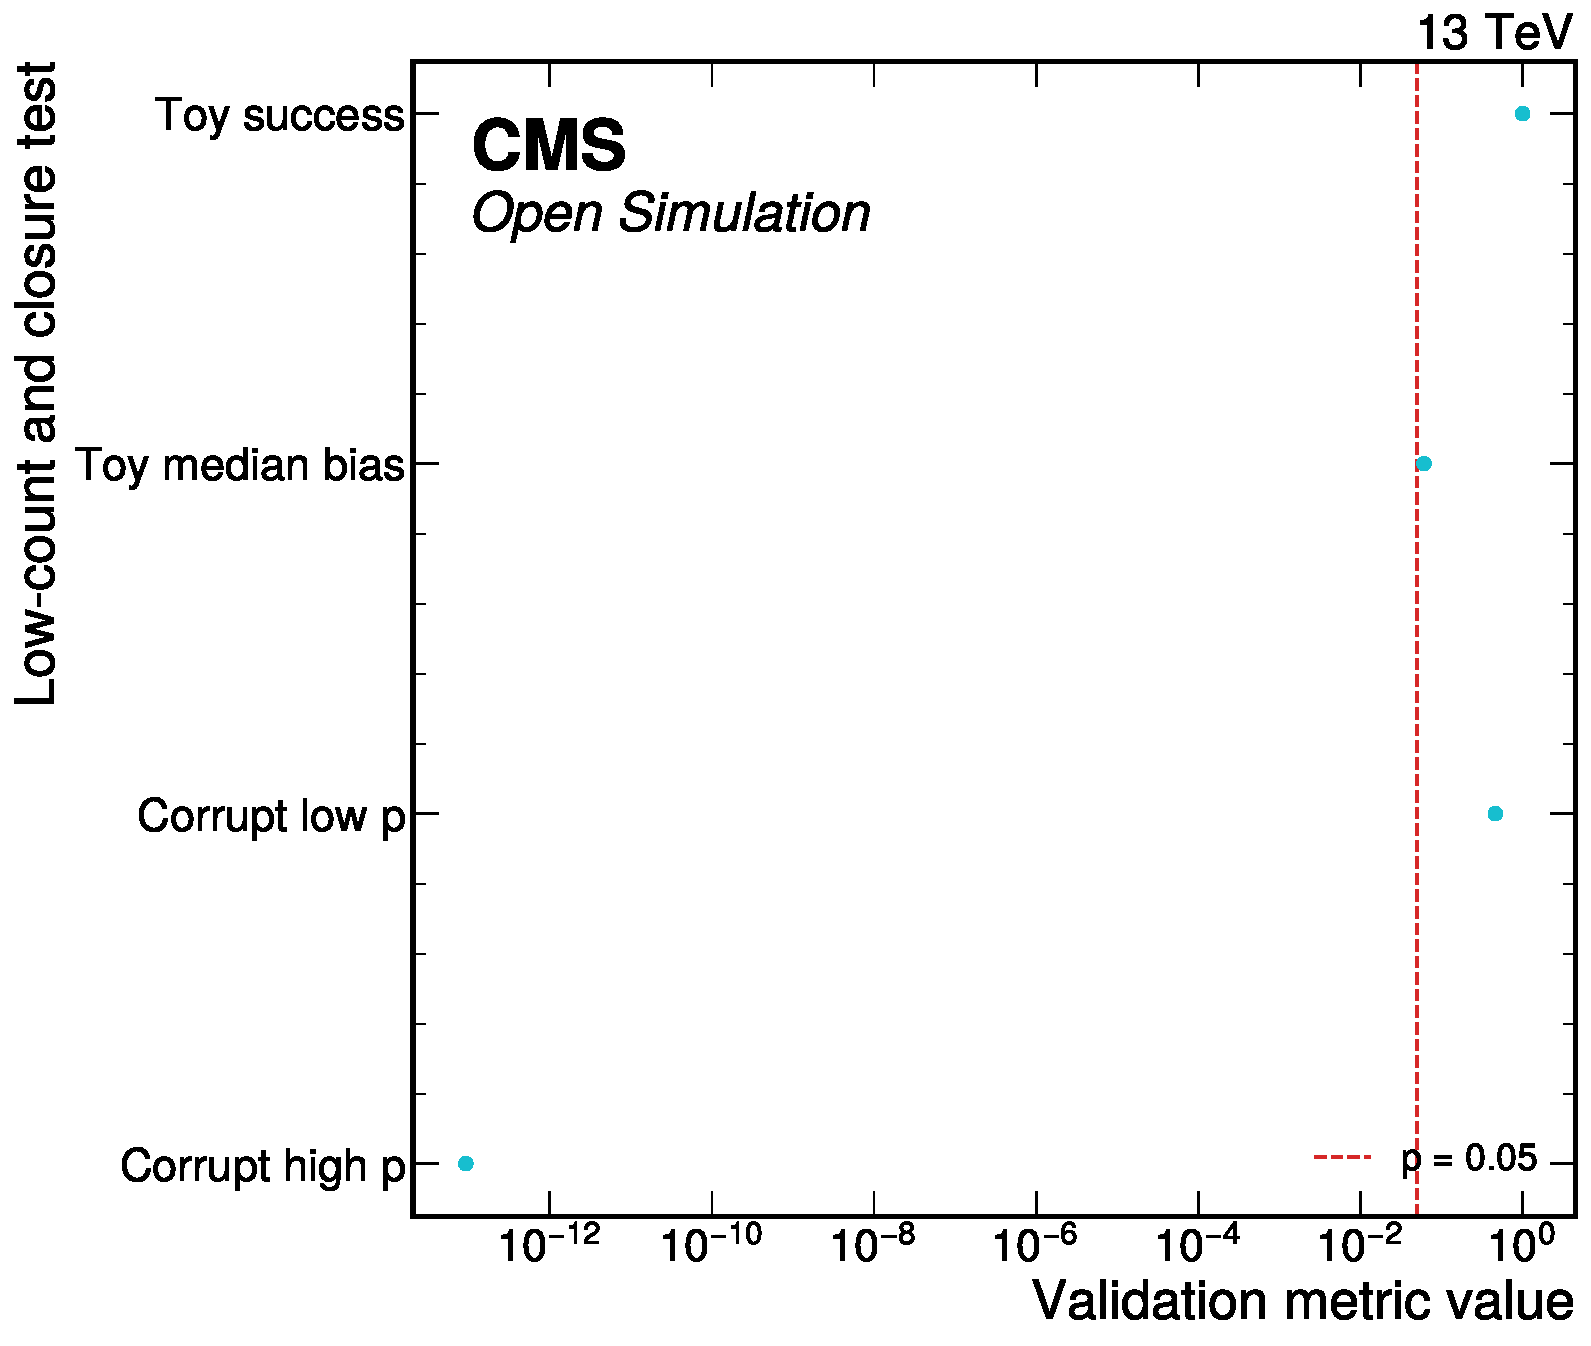
\includegraphics[width=0.92\linewidth,height=0.70\textheight,keepaspectratio]{figures/expected_low_count_validation.pdf}
\caption{Expected low-count toy and closure-sensitivity validation summary. The final-state simultaneous corruption test rejects the +20 percent mass-response case; the -20 percent case is retained as a documented low-count sensitivity limitation in the JSON.}
\label{fig:expected-low-count-validation}
\end{figure}

\begin{figure}[p]
\centering
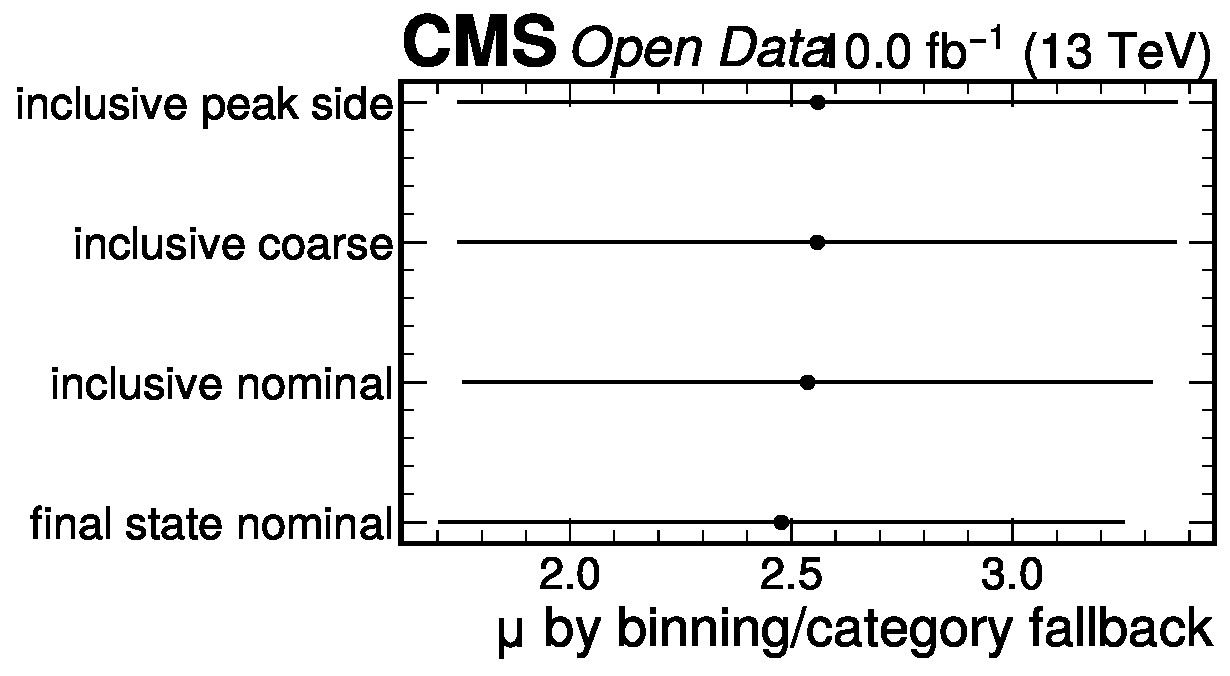
\includegraphics[width=0.92\linewidth,height=0.70\textheight,keepaspectratio]{figures/observed_binning_stability.pdf}
\caption{Full-data low-count stability check comparing the nominal final-state binning with inclusive and coarser alternatives. All variants give compatible central values near $\mu\simeq2.5$ with acceptable GoF p-values, supporting the retained S1 final-state model.}
\label{fig:observed-binning-stability}
\end{figure}

\begin{figure}[p]
\centering
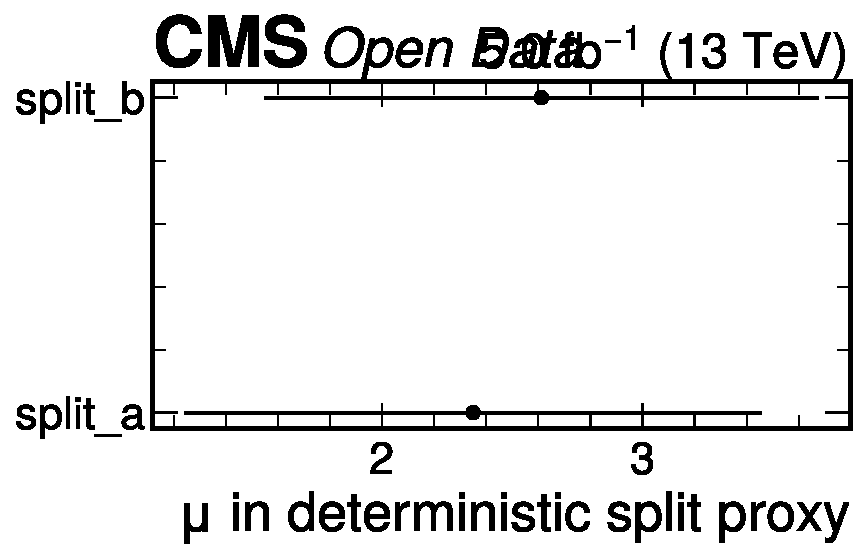
\includegraphics[width=0.92\linewidth,height=0.70\textheight,keepaspectratio]{figures/observed_split_consistency.pdf}
\caption{Deterministic half-split proxy consistency check for the full observed sample. The two halves differ by a pull of -0.171, but this is explicitly a proxy because true CMS run-period branches are unavailable.}
\label{fig:observed-split-consistency}
\end{figure}

\begin{figure}[p]
\centering
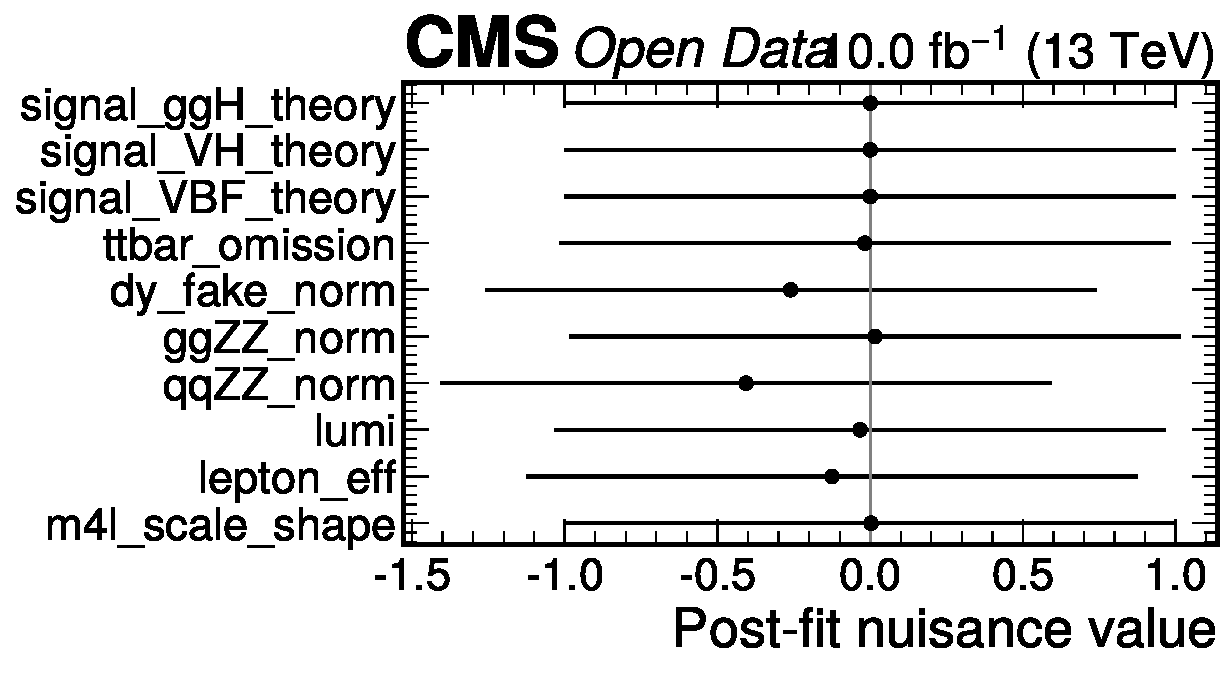
\includegraphics[width=0.92\linewidth,height=0.70\textheight,keepaspectratio]{figures/observed_nuisance_pulls.pdf}
\caption{Observed full-data nuisance best-fit values for the nominal final-state workspace. The pulls do not show a pathological constraint pattern, and they are interpreted with the DY fake-proxy and grouped MC-stat limitations documented in the text.}
\label{fig:observed-nuisance-pulls}
\end{figure}

\begin{figure}[p]
\centering
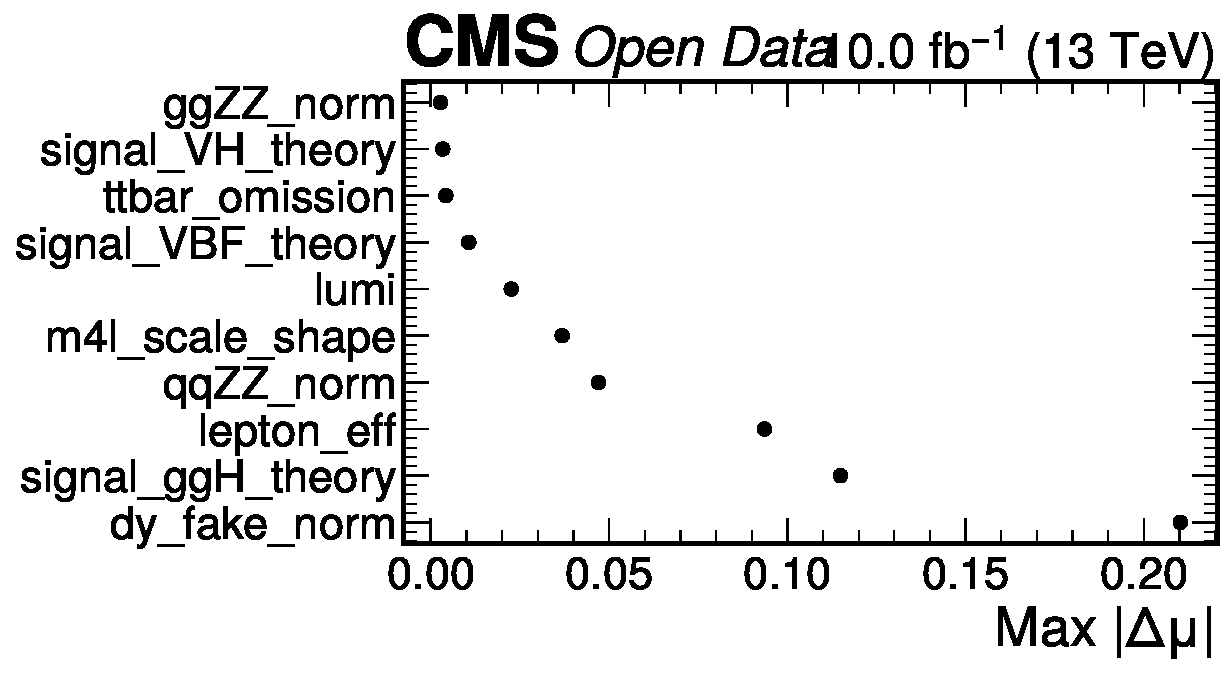
\includegraphics[width=0.92\linewidth,height=0.70\textheight,keepaspectratio]{figures/observed_nuisance_impacts.pdf}
\caption{Largest fixed-nuisance impacts on the full-data signal-strength fit. The dominant impact is the DY fake-proxy normalization at about 0.210 in $\mu$, followed by signal-theory and lepton-efficiency sources; the measurement remains statistically limited.}
\label{fig:observed-nuisance-impacts}
\end{figure}

\begin{figure}[p]
\centering
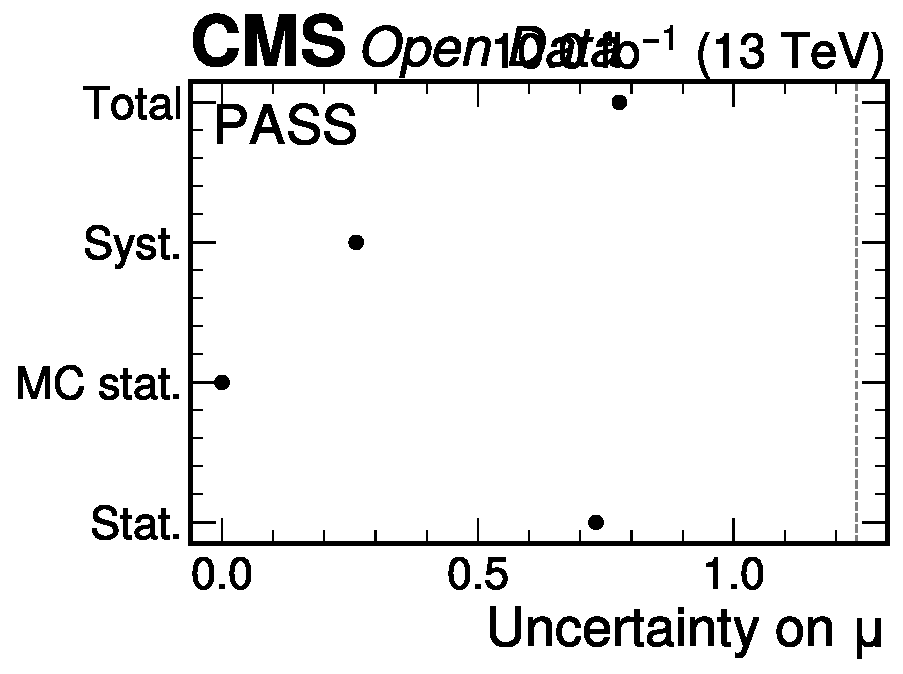
\includegraphics[width=0.92\linewidth,height=0.70\textheight,keepaspectratio]{figures/observed_uncertainty_viability.pdf}
\caption{Full-data uncertainty and viability summary. The relative total uncertainty is 0.313 and the fit triviality gate passes, so the observed result is reportable within the detector-level scope even though it is not competitive with official CMS precision.}
\label{fig:observed-uncertainty-viability}
\end{figure}

\subsection{Phase 4b Partial-Data Stability}
The fixed-seed 10\% result remains a validation cross-check. It used the same broad $70 < m_{4\ell} < 170$ GeV fit window and retained final-state categories, but the best fit landed at the physical boundary with $\mu=0.0^{+1.3549}$. The full-data result is compatible with this partial result at 1.587 standard deviations, so the partial boundary behavior is not used to retune the model.

\begin{table}[htbp]
\centering
\caption{Phase 4b fixed-seed 10\% validation summary from partial\_parameters.json.}
\begin{tabular}{ll}
\toprule
Quantity & Value \\
\midrule
Random seed & 9417 \\
Selected events kept & 20 / 203 \\
Effective luminosity & 1.0 fb$^{-1}$ \\
Fit window & 70--170 GeV \\
Channel counts & 2e2mu: 10, 4e: 3, 4mu: 7 \\
$\hat{\mu}$ & $0.0^{+1.3549}$, lower interval at boundary \\
$\chi^2/\mathrm{ndf}$ & 31.755 / 38 \\
$p(\chi^2)$ & 0.7524 \\
Pull vs full-data result & 1.587 \\
\bottomrule
\end{tabular}
\label{tab:partial-validation-summary}
\end{table}

\begin{figure}[p]
\centering
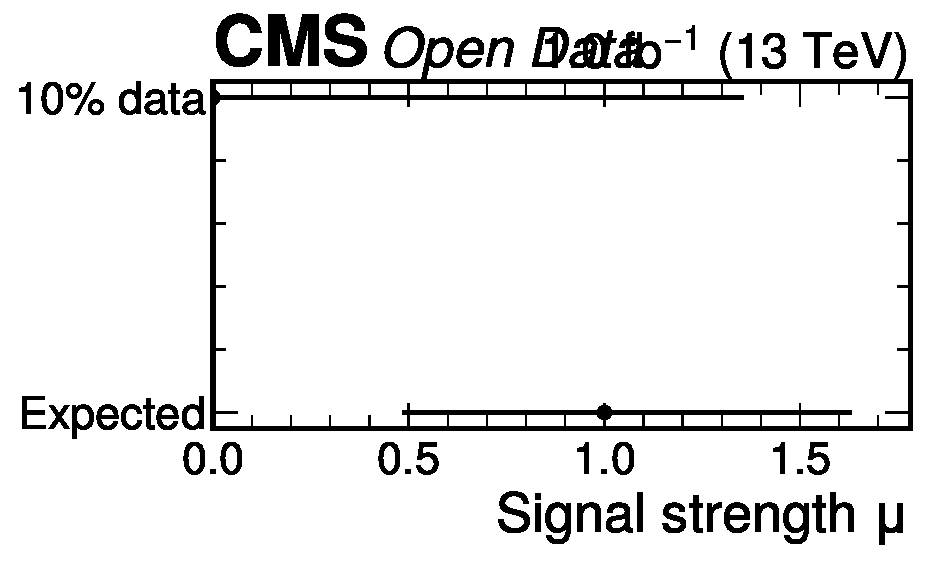
\includegraphics[width=0.92\linewidth,height=0.70\textheight,keepaspectratio]{figures/partial_expected_mu_comparison.pdf}
\caption{Phase 4b 10\% signal-strength comparison retained as validation history. The partial-data best fit lands at the physical boundary $\mu=0$, but its broad uncertainty makes it compatible with both the expected baseline and the full-data result.}
\label{fig:partial-expected-mu-comparison}
\end{figure}

\begin{figure}[p]
\centering
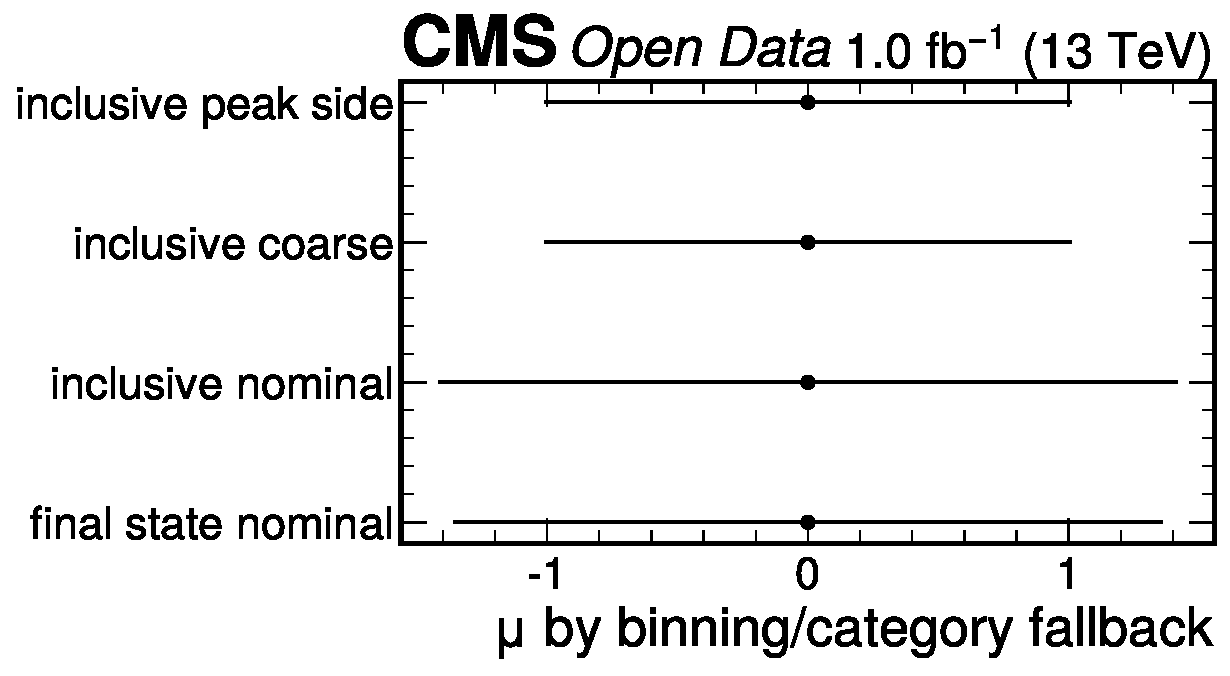
\includegraphics[width=0.92\linewidth,height=0.70\textheight,keepaspectratio]{figures/partial_binning_stability.pdf}
\caption{Phase 4b low-count stability check comparing the nominal final-state binning with inclusive and coarser alternatives. It is retained as a validation cross-check rather than a primary result figure.}
\label{fig:partial-binning-stability}
\end{figure}

\section{Statistical Method}
The nominal inference uses a binned simultaneous template likelihood implemented with pyhf \cite{pyhf_joss,HistFactory}. One global parameter of interest $\mu$ scales all Higgs production templates together. The active channels are $4\mu$, $4e$, and $2e2\mu$, and the active signal-strength fit window is $70 < m_{4\ell} < 170$ GeV for Phase 4a expected, Phase 4b partial, and Phase 4c observed results.

The broad-window mass-bin edges are
\begin{equation}
\begin{split}
&[70,80,90,100,105,112,118,\\
&\quad 122,126,130,140,150,160,170]\ \mathrm{GeV}.
\end{split}
\end{equation}
This window intentionally includes the Z peak because it is the user-directed current configuration and because the same broad-window template handoff is now used consistently across the expected, partial, and full observed phases. CMS public-reference methods may use a narrower $105<m_{4\ell}<140$ GeV signal region; that is a reference-method difference, not the current fit-window definition.

The likelihood is
\begin{equation}
 L(\mu,\boldsymbol{\theta}) =
 \prod_{c,b}\mathrm{Pois}\!\left(n_{cb}\mid \lambda_{cb}(\mu,\boldsymbol{\theta})\right)
 \prod_k \pi_k(\theta_k),
 \label{eq:likelihood}
\end{equation}
where $\pi_k$ are Gaussian or log-normal constraints depending on the modifier. The profile-likelihood test statistic is
\begin{equation}
 q(\mu) = -2\log\frac{L(\mu,\hat{\hat{\boldsymbol{\theta}}}_{\mu})}{L(\hat{\mu},\hat{\boldsymbol{\theta}})}.
 \label{eq:profile}
\end{equation}
The one-sigma interval is read from $\Delta q(\mu)=1$ on the profile scan. Asymptotic profile-likelihood methods and numerical minimization tools are standard for HEP measurements \cite{Cowan2011,Minuit}, but the low expected bin counts are why the note also reports toy and binning-stability diagnostics \cite{Cowan2011}.

The parameter convention is deliberately simple. A single global signal-strength POI multiplies all Higgs production components, so the fit measures the total Higgs yield relative to the nominal prompt-normalized MC expectation. The production-mode labels are retained inside the template model only so that signal-composition uncertainties can be propagated. They are not independent POIs, and the note does not quote ggH, VBF, or VH signal strengths.

The nuisance parameters are interpreted differently in expected and observed phases. In Phase 4a the Asimov pseudo-data are generated from the same nominal model that is fitted, so nuisance best fits at nominal values are expected. In Phase 4c the nuisance pulls and impacts are observed-data diagnostics; the largest impact is the DY fake-proxy normalization at 0.210 in $\mu$, followed by signal-theory and lepton-efficiency sources.

The mass-profile scan uses the same broad likelihood structure for observed counts and background constraints, but the Higgs mass-hypothesis grid excludes the Z-peak region. It replaces the signal template at each grid mass with a shifted detector-level M125-derived template and profiles $\mu$ at each grid point. The scan is method-parity evidence, not a calibrated mass measurement, because independent mass-hypothesis MC and official per-lepton calibration/morphing inputs are unavailable.

\section{Results}
The full observed dataset is the primary Doc 4c result. It retains all 203 selected events at the full 10 fb$^{-1}$ normalization and uses the active $70 < m_{4\ell} < 170$ GeV fit window in the final-state categories. The 10\% sample is now a validation cross-check, and the Phase 4a Asimov result is the expected baseline.

\begin{table}[htbp]
\centering
\caption{Signal-strength results from the machine-readable JSON files. The full-data row is the primary result; the 10\% row is a validation cross-check.}
\begin{tabular}{lllll}
\toprule
Stage & Fit window [GeV] & $\hat{\mu}$ & $-1\sigma$ & $+1\sigma$ \\
\midrule
Phase 4a expected & 70--170 & 1.0000 & 0.5109 & 0.6265 \\
Phase 4b 10\% observed & 70--170 & 0.0000 & boundary & 1.3549 \\
Phase 4c full observed & 70--170 & 2.4776 & 0.7139 & 0.8388 \\
\bottomrule
\end{tabular}
\label{tab:mu-result}
\end{table}

\begin{table}[htbp]
\centering
\caption{Full-data fit summary from observed\_parameters.json and observed\_validation.json. MC templates use the full 10 fb$^{-1}$ normalization and no component is normalized to the observed data integral.}
\begin{tabular}{ll}
\toprule
Quantity & Value \\
\midrule
Selected events kept & 203 / 203 \\
Effective luminosity & 10.0 fb$^{-1}$ \\
Channel counts & 2e2mu: 98, 4e: 24, 4mu: 81 \\
$\hat{\mu}$ & $2.4776^{+0.8388}_{-0.7139}$ \\
Symmetric uncertainty & 0.7763 \\
$\chi^2/\mathrm{ndf}$ & 47.326 / 38 \\
$p(\chi^2)$ & 0.1427 \\
Poisson deviance / p-value & 48.685 / 0.1148 \\
Expected-vs-observed pull & 1.535 \\
Partial-vs-observed pull & 1.587 \\
Fit triviality gate & PASS \\
Viability verdict & PASS \\
\bottomrule
\end{tabular}
\label{tab:observed-gof}
\end{table}

\begin{table}[htbp]
\centering
\caption{Full-data variance decomposition for $\mu$ from observed\_covariance.json. The grouped MC-stat treatment remains the reviewed approximation and is not a full bin-by-bin HistFactory staterror profile.}
\begin{tabular}{lll}
\toprule
Component & Variance & Uncertainty \\
\midrule
Statistical & 0.53397 & 0.7307 \\
MC statistical approximation & 0.00000 & 0.0000 \\
Systematic including MC stat & 0.06873 & 0.2622 \\
Total & 0.60270 & 0.7763 \\
\bottomrule
\end{tabular}
\label{tab:variance}
\end{table}

\begin{figure}[p]
\centering
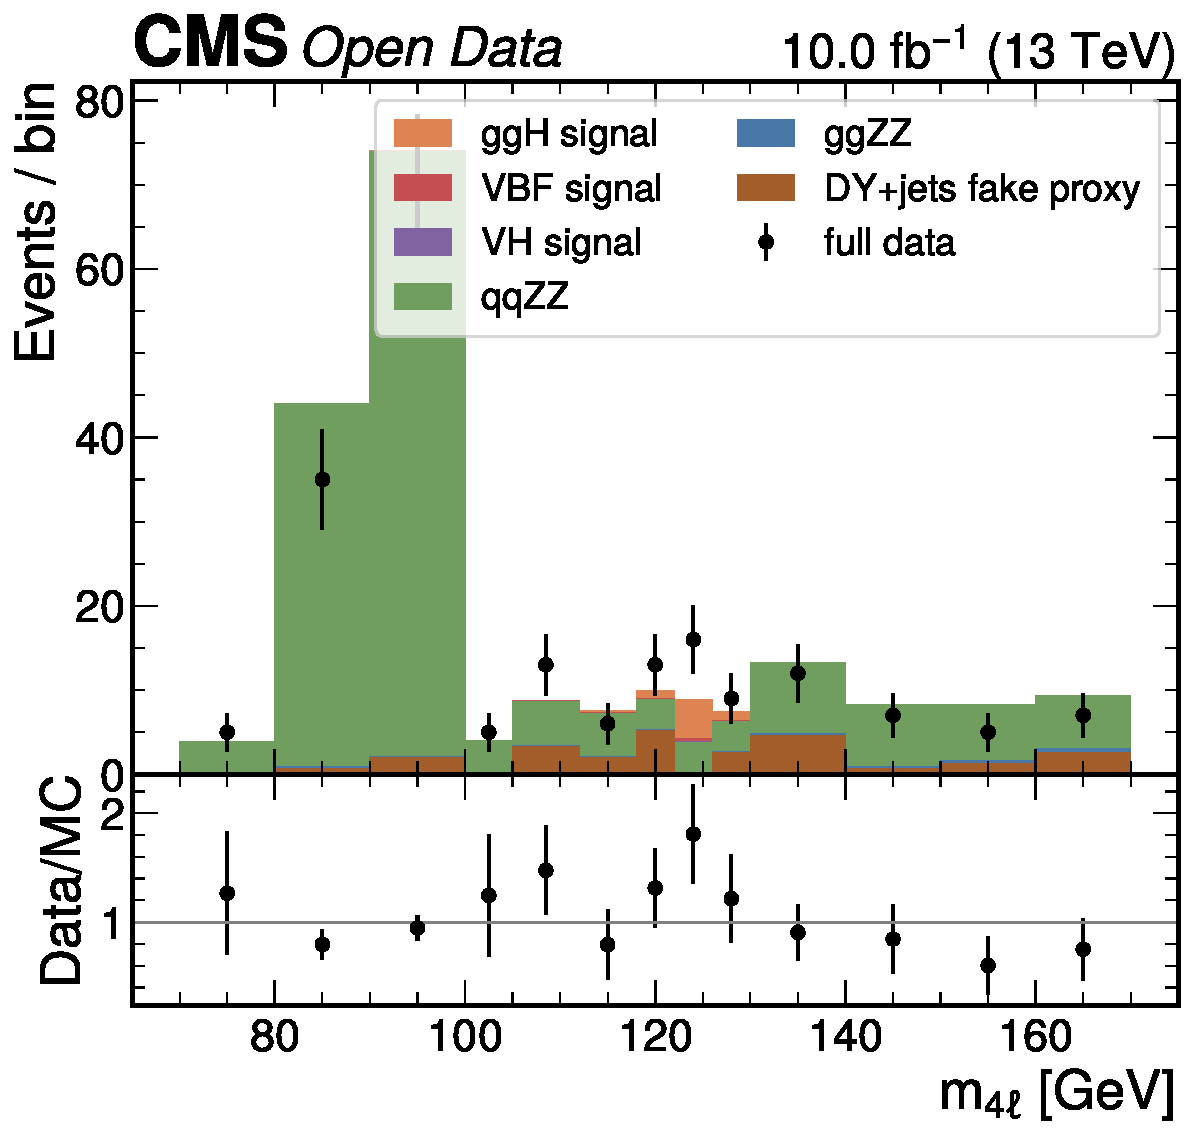
\includegraphics[width=0.92\linewidth,height=0.70\textheight,keepaspectratio]{figures/observed_m4l_broad_inclusive.pdf}
\caption{Full-data four-lepton mass distribution in the active $70 < m_{4\ell} < 170$ GeV fit window. The display includes the Z peak and compares all selected observed events with prompt-normalized MC; no component is normalized to the observed data integral.}
\label{fig:observed-m4l-broad-inclusive}
\end{figure}

\begin{figure}[p]
\centering
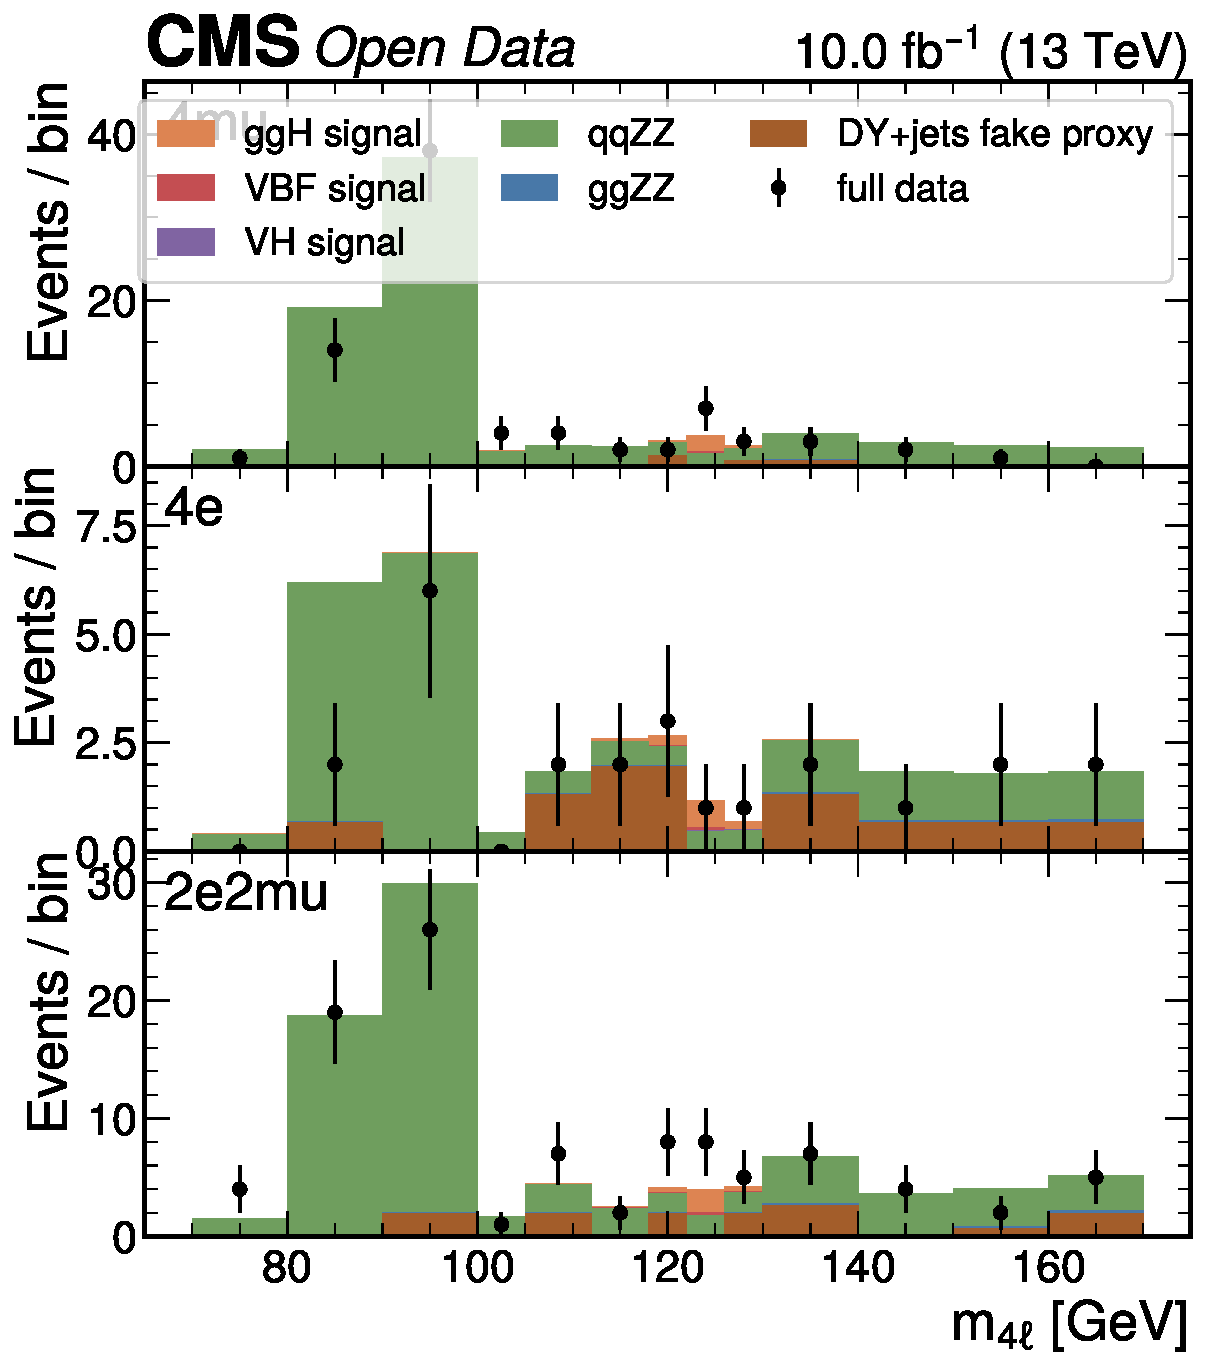
\includegraphics[width=0.92\linewidth,height=0.70\textheight,keepaspectratio]{figures/observed_m4l_70_170_categories.pdf}
\caption{Full-data final-state templates in the $70 < m_{4\ell} < 170$ GeV fit window. The nominal categories are $4\mu$, $4e$, and $2e2\mu$ only; VBF is formally downscoped because no recoverable jet/VBF information exists in the allowed flat ntuples.}
\label{fig:observed-m4l-70-170-categories}
\end{figure}

\begin{figure}[p]
\centering
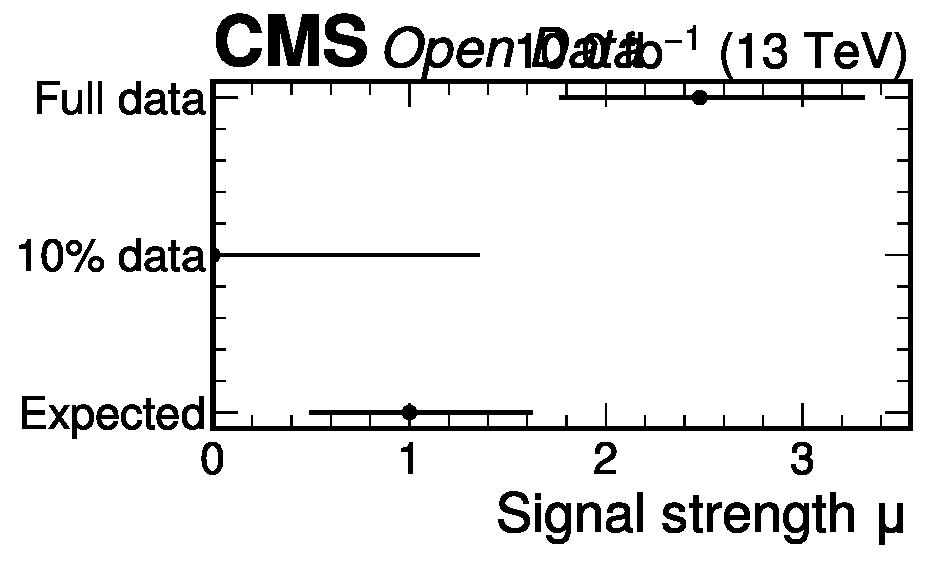
\includegraphics[width=0.92\linewidth,height=0.70\textheight,keepaspectratio]{figures/observed_expected_mu_comparison.pdf}
\caption{Expected, 10\%, and full-data signal-strength comparison. The full-data value $\mu=2.4776^{+0.8388}_{-0.7139}$ is compatible with the Phase 4a expected baseline at 1.535 standard deviations and with the 10\% validation result at 1.587 standard deviations.}
\label{fig:observed-expected-mu-comparison}
\end{figure}

\begin{figure}[p]
\centering
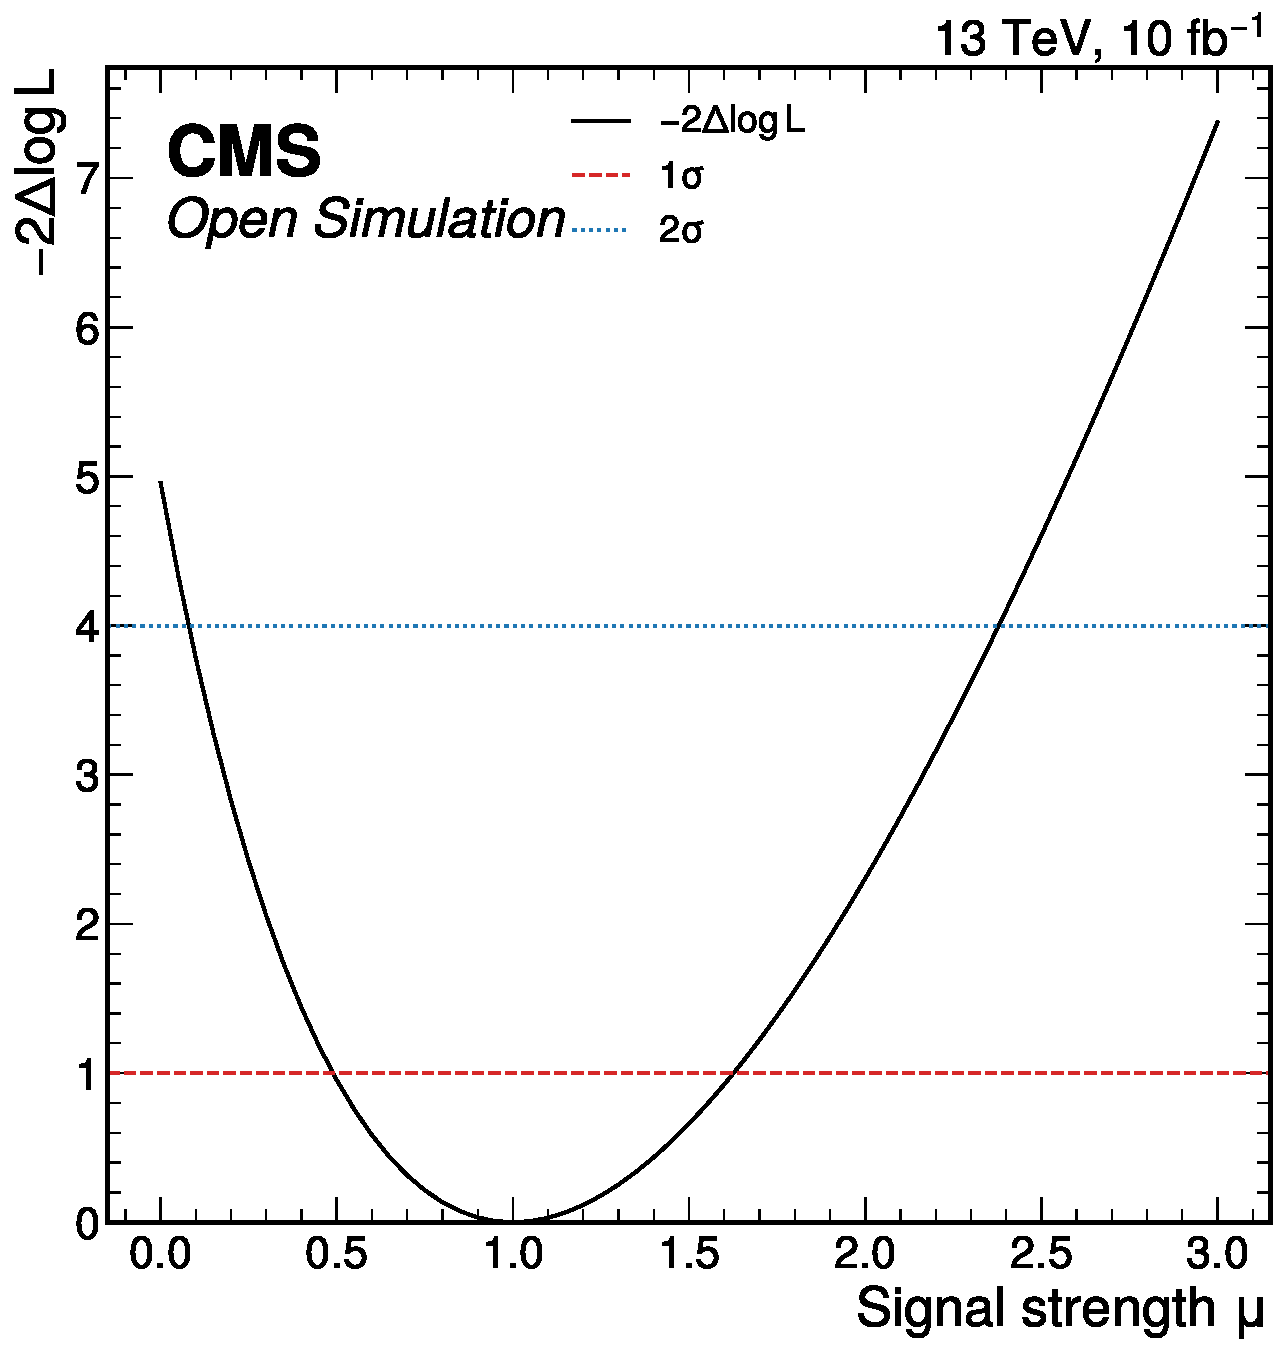
\includegraphics[width=0.92\linewidth,height=0.70\textheight,keepaspectratio]{figures/expected_mu_profile_scan.pdf}
\caption{Expected profile-likelihood scan for the global Higgs signal-strength parameter. The broad-window Asimov best fit is $\mu=1$ with symmetric expected uncertainty 0.5687, providing the expected baseline for the full-data comparison.}
\label{fig:expected-mu-profile-scan}
\end{figure}

\begin{figure}[p]
\centering
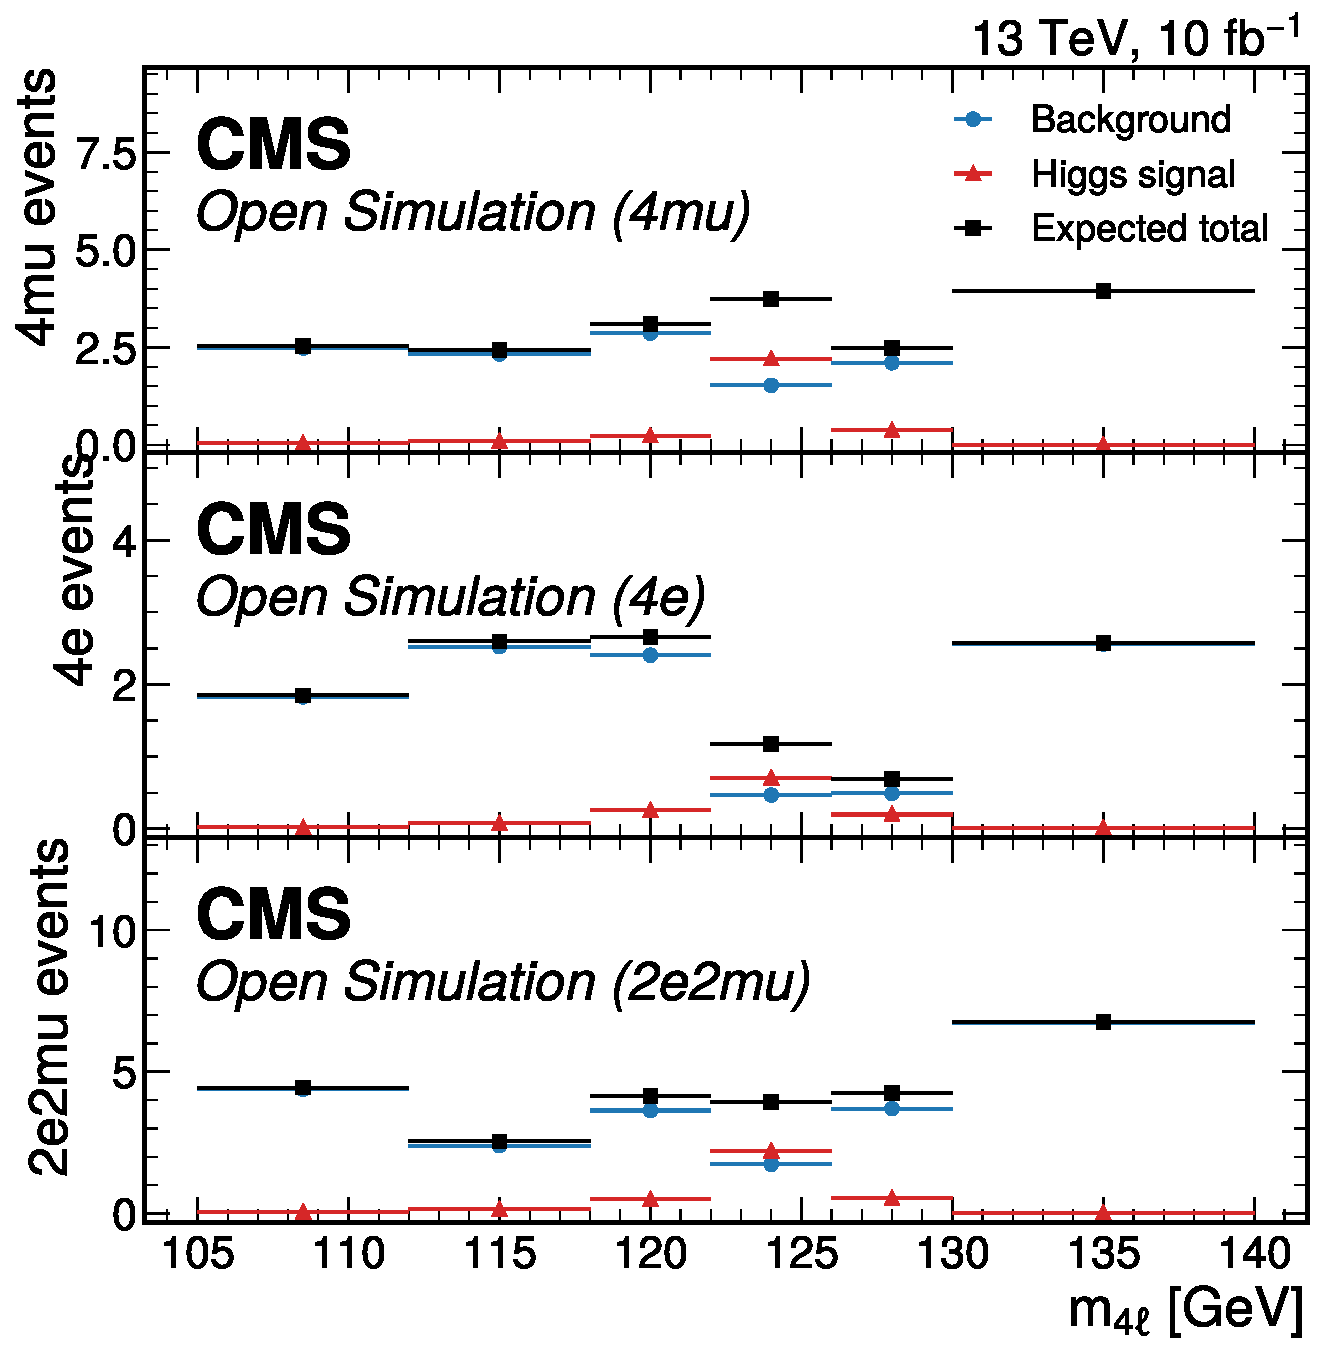
\includegraphics[width=0.92\linewidth,height=0.70\textheight,keepaspectratio]{figures/expected_m4l_final_state_templates.pdf}
\caption{Expected Asimov four-lepton mass templates in the final-state categories used by the broad-window simultaneous fit. Points show the background expectation, Higgs signal expectation, and their total; observed Open Data counts are introduced only in the partial and full observed phases.}
\label{fig:expected-m4l-final-state-templates}
\end{figure}

\subsection{Mass-Profile Diagnostic}
The observed shifted-template mass scan uses the broad likelihood for observed counts and background constraints, while excluding the Z-peak region from Higgs mass hypotheses. It first scans $110$--$150$ GeV in 2.5 GeV steps, then refines locally over $122$--$128$ GeV in 0.25 GeV steps around the coarse minimum. The fine-grid center is $m_H=124.75$ GeV with profiled $\mu=2.4035$. The diagnostic $\Delta(-2\ln L)\le1$ grid interval is $[124.75,125.50]$ GeV, but this is a shifted-template grid diagnostic rather than a calibrated statistical uncertainty. A quadratic interpolation of the fine-grid points gives $125.424$ GeV and is retained only as a diagnostic interpolation, not as the reported center.

\begin{table}[htbp]
\centering
\caption{Observed shifted-template mass scan from observed\_mass\_scan.json. The scan is detector-level diagnostic evidence and is not promoted to an official mass measurement.}
\begin{tabular}{ll}
\toprule
Quantity & Value \\
\midrule
Coarse scan range & 110--150 GeV in 2.5 GeV steps \\
Fine scan range & 122--128 GeV in 0.25 GeV steps \\
Coarse best grid point & 125.0 GeV \\
Reported fine-grid center & 124.75 GeV \\
Best profiled $\mu$ in mass scan & 2.4035 \\
Diagnostic grid half-step & 0.125 GeV, not stat/syst \\
Diagnostic grid interval & [124.75, 125.50] GeV by $\Delta(-2\ln L)\le1$ grid criterion \\
Diagnostic quadratic interpolation & 125.424 GeV, not reported as calibrated center \\
Promoted to nominal mass measurement & no \\
Z-peak treatment & excluded from Higgs mass-hypothesis grid \\
\bottomrule
\end{tabular}
\label{tab:observed-mass-scan}
\end{table}

\begin{figure}[p]
\centering
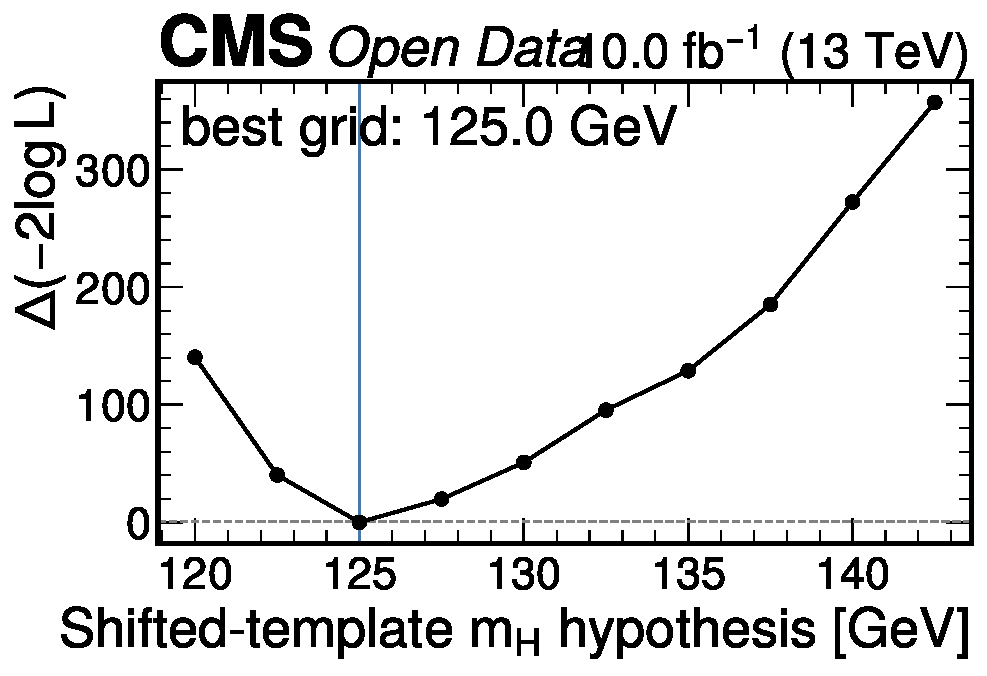
\includegraphics[width=0.92\linewidth,height=0.70\textheight,keepaspectratio]{figures/observed_mass_scan.pdf}
\caption{Observed shifted-template detector-level mass scan with $\mu$ profiled at each mass hypothesis. The coarse scan is refined locally with a 0.25 GeV grid, giving a reported fine-grid center of 124.75 GeV. The scan is not an official CMS-quality mass measurement because independent mass-hypothesis MC and official calibration/morphing inputs are unavailable.}
\label{fig:observed-mass-scan}
\end{figure}

\section{Comparison to Prior Results and Theory}
The full-data result is compared quantitatively with public CMS and PDG references as context, not as a tuning target. The comparison is not methodologically one-to-one: this note uses open-data flat ntuples, S1 final-state categories, a broad $70 < m_{4\ell} < 170$ GeV signal-strength fit window, DY+jets as the reducible fake proxy, and no official lepton calibration or data-driven Z+X estimate. CMS-HIG-16-041 and CMS-HIG-19-001 use official CMS calibrations, production-sensitive categories, and different background treatments.

Using a symmetrized CMS-HIG-16-041 uncertainty of 0.18, the full-data signal-strength pull is $(2.4776-1.05)/\sqrt{0.7763^2+0.18^2}=1.79$ standard deviations, and the central-value ratio is 2.36. Using a combined CMS-HIG-19-001 uncertainty of $\sqrt{0.07^2+0.085^2}=0.110$, the pull is 1.96 standard deviations, and the central-value ratio is 2.64. The precision ratio relative to CMS-HIG-16-041 is $0.7763/0.18=4.31$; relative to the approximate CMS-HIG-19-001 combined uncertainty it is 7.05.

The observed mass-scan fine-grid center is 124.75 GeV. CMS-HIG-16-041/JHEP 11 (2017) 047 reports $m_H=125.26\pm0.20\mathrm{(stat)}\pm0.08\mathrm{(syst)}$ GeV, giving a quadrature total uncertainty of 0.215 GeV \cite{CMS-HIG-16-041}. The PDG 2024 world-average context value is $125.20\pm0.11$ GeV \cite{PDG2024}. The grid residuals are -0.51 GeV and -0.45 GeV, respectively, but no calibrated pull is quoted for this analysis because the scan uses shifted M125 templates and has no meaningful statistical/systematic split.

\begin{table}[htbp]
\centering
\caption{Comparison matrix. Non-comparable entries are explicitly labeled; public CMS values are contextual references only and are not targets for tuning.}
\begin{small}
\begin{tabular}{p{0.17\linewidth}p{0.23\linewidth}p{0.31\linewidth}p{0.19\linewidth}}
\toprule
Quantity & This Doc 4c note & Reference & Quantitative comparison \\
\midrule
Inclusive $\mu$ & $2.4776^{+0.8388}_{-0.7139}$ & CMS-HIG-16-041: $1.05^{+0.19}_{-0.17}$ & pull 1.79$\sigma$, ratio 2.36, uncertainty ratio 4.31 \\
Inclusive $\mu$ & $2.4776^{+0.8388}_{-0.7139}$ & CMS-HIG-19-001: $0.94\pm0.07\mathrm{(stat)}^{+0.09}_{-0.08}\mathrm{(syst)}$ & pull 1.96$\sigma$, ratio 2.64, uncertainty ratio 7.05 \\
Internal compatibility & pull = 1.535 & Phase 4a expected baseline & compatible within two standard deviations \\
10\% validation compatibility & pull = 1.587 & Phase 4b fixed-seed validation & compatible within two standard deviations \\
Mass diagnostic & 124.75 GeV fine-grid center; 0.125 GeV grid half-step, not stat/syst & CMS-HIG-16-041: $125.26\pm0.20\mathrm{(stat)}\pm0.08\mathrm{(syst)}$ GeV & residual -0.51 GeV; no calibrated pull quoted \\
Mass diagnostic & 124.75 GeV fine-grid center; 0.125 GeV grid half-step, not stat/syst & PDG 2024: $125.20\pm0.11$ GeV world average & residual -0.45 GeV; no calibrated pull quoted \\
Fiducial cross section & not extracted & CMS-HIG-16-041 and CMS-HIG-19-001 fiducial results & unavailable in this detector-level analysis \\
Width & not extracted & CMS-HIG-16-041: $\Gamma_H<1.10$ GeV & unavailable \\
VBF categories & downscoped & CMS production-sensitive categories & unavailable without jets \\
Reducible background & DY+jets MC proxy & CMS data-driven Z+X & approximated \\
\bottomrule
\end{tabular}
\end{small}
\label{tab:comparison}
\end{table}

\begin{figure}[p]
\centering
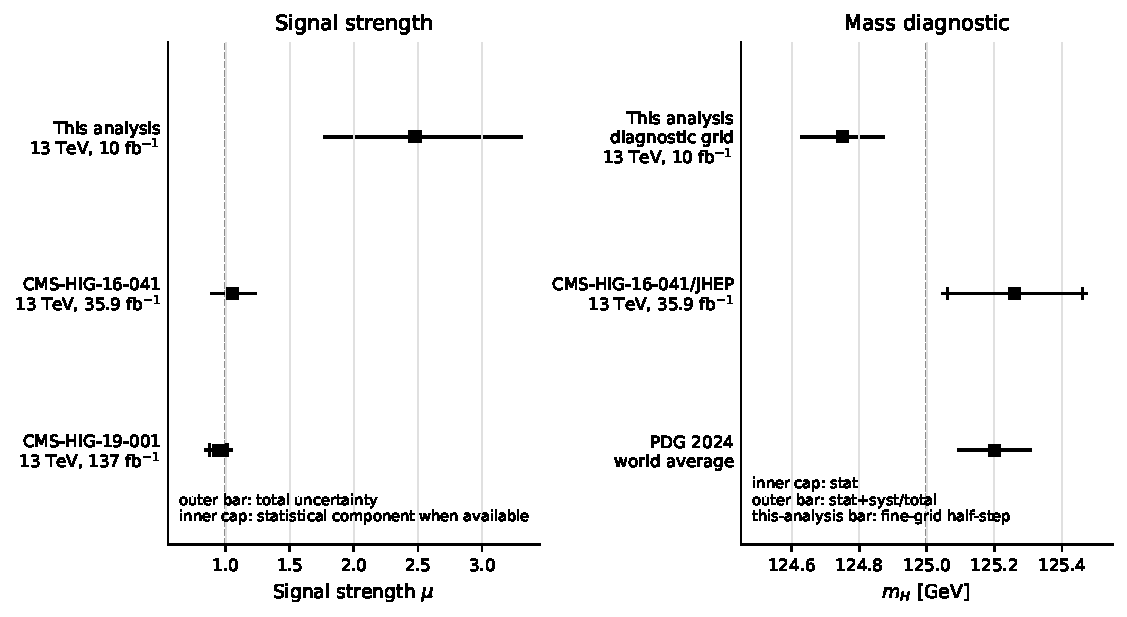
\includegraphics[width=0.92\linewidth,height=0.70\textheight,keepaspectratio]{figures/doc4c_reference_comparison.pdf}
\caption{Full-data signal-strength and mass-diagnostic comparison with public CMS and PDG references. This comparison figure is part of the main result narrative; the labels state the center-of-mass energy and luminosity for dataset-specific entries, while the PDG entry is labeled as a world average. The signal-strength pulls are 1.79 standard deviations relative to CMS-HIG-16-041 and 1.96 standard deviations relative to CMS-HIG-19-001. In the mass panel, CMS-HIG-16-041 uses an inner capped horizontal bar for the statistical uncertainty and an uncapped horizontal systematic component; this analysis is shown only with a diagnostic fine-grid half-step because no stat/syst split is calibrated for the shifted-template scan.}
\label{fig:doc4c-reference-comparison}
\end{figure}

\begin{figure}[p]
\centering
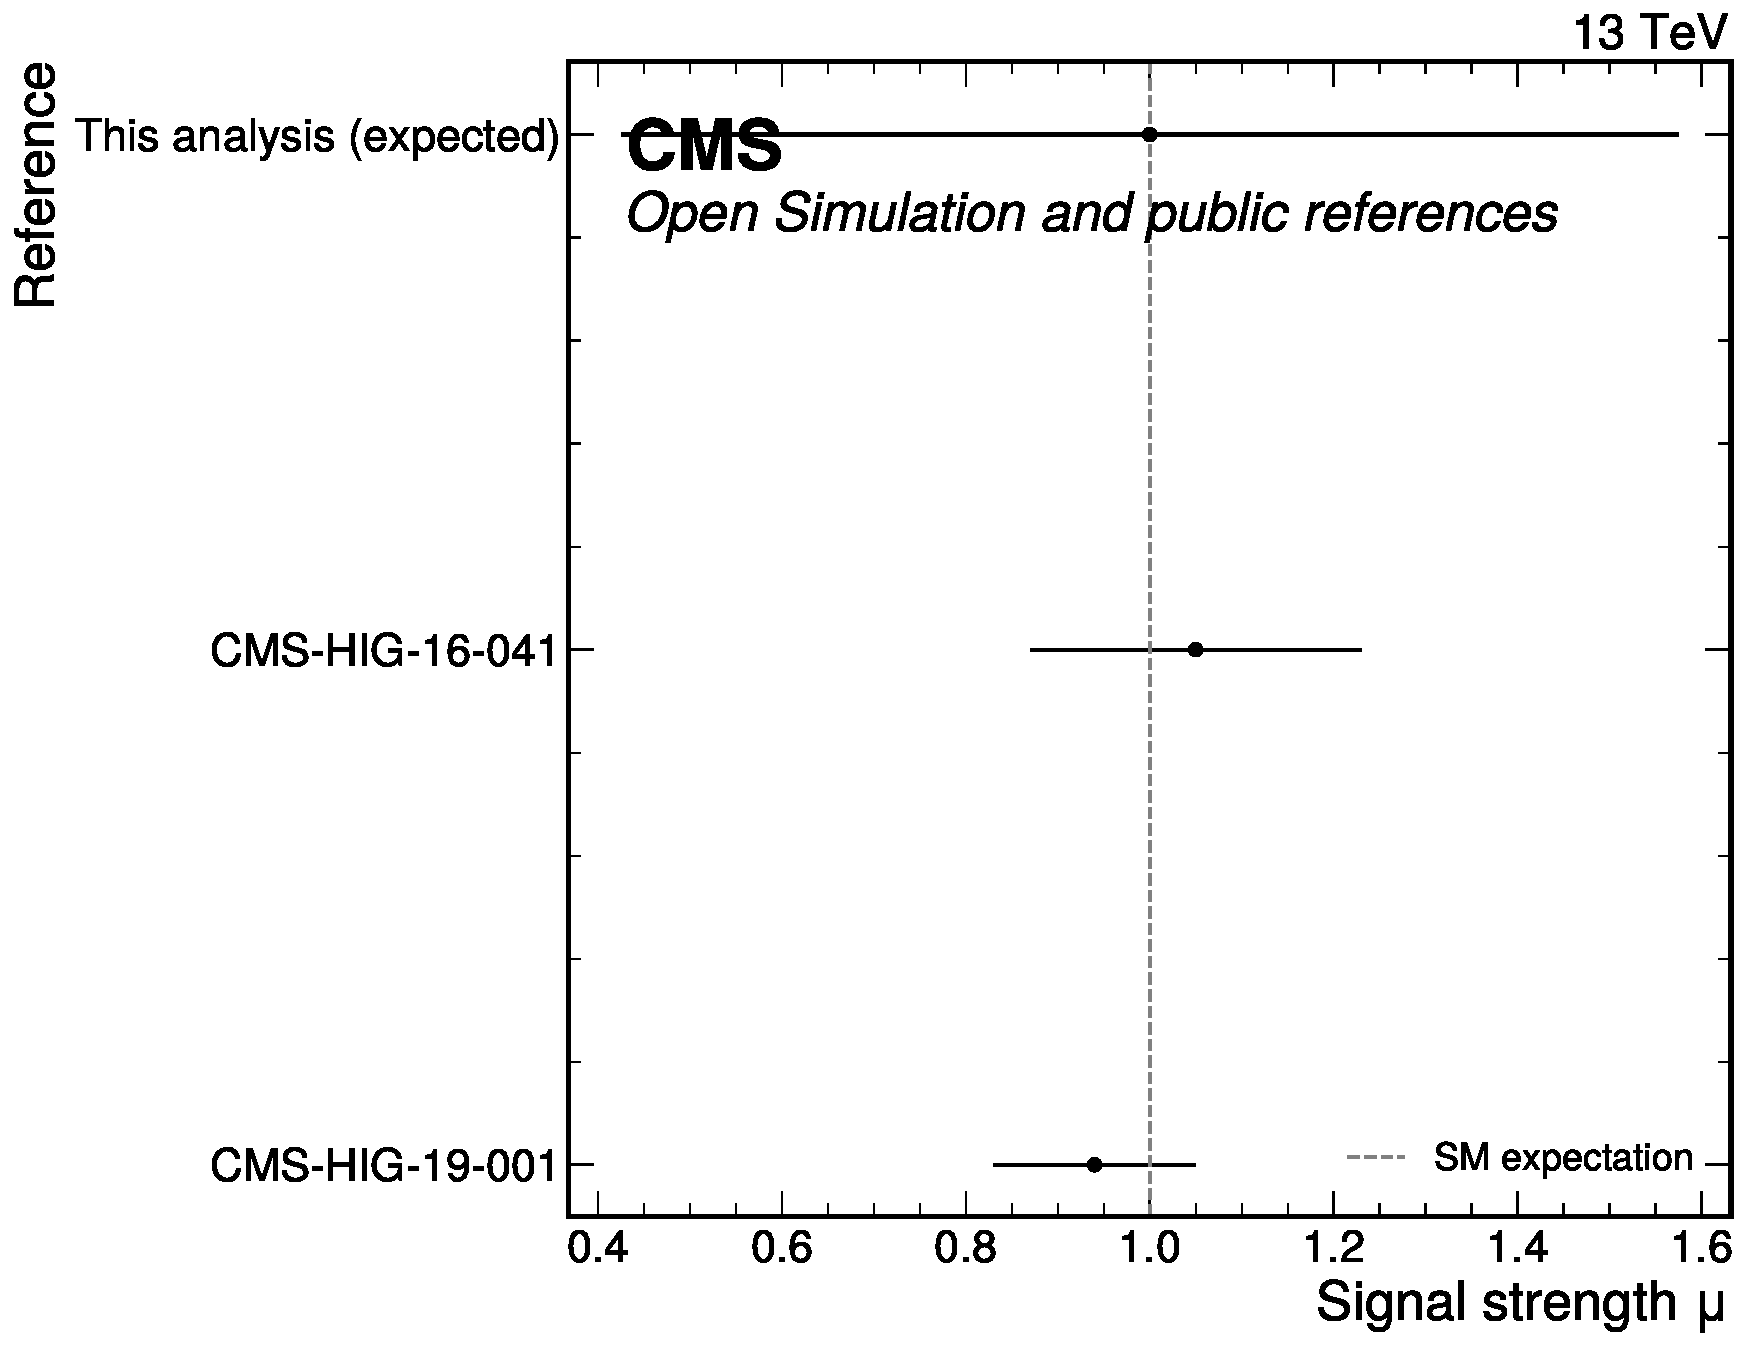
\includegraphics[width=0.92\linewidth,height=0.70\textheight,keepaspectratio]{figures/expected_reference_comparison.pdf}
\caption{Expected Phase 4a signal-strength precision compared with public CMS H to ZZ to four-lepton references. This expected-only comparison is retained for continuity; the primary full-data comparison is shown in Fig.~\ref{fig:doc4c-reference-comparison}.}
\label{fig:expected-reference-comparison}
\end{figure}

\section{Conclusions}
The final Doc 4c detector-level open-data result is $\mu=2.4776^{+0.8388}_{-0.7139}$ in the active $70<m_{4\ell}<170$ GeV final-state template fit. The post-fit goodness of fit is non-pathological, $\chi^2/\mathrm{ndf}=47.326/38$ with $p=0.1427$, and the fit triviality gate passes. The result is compatible with the Phase 4a expected baseline at 1.535 standard deviations and with the fixed-seed 10\% validation result at 1.587 standard deviations.

The measurement is honest about its scope. It is detector-level, statistically limited, and not competitive with official CMS precision: the uncertainty is 4.31 times the symmetrized CMS-HIG-16-041 uncertainty. The dominant data-sensitive nuisance impact is the DY fake-proxy normalization, while the total variance is dominated by statistical uncertainty. The shifted-template mass scan finds a refined fine-grid center at 124.75 GeV, but it remains a diagnostic because the analysis lacks independent mass-hypothesis MC and official calibration inputs.

VBF and MVA categories are not part of the nominal result. The allowed flat ntuples do not contain recoverable jet or VBF information, so VBF is formally downscoped. The repaired MVA is no longer random and reaches useful broad-window separation, but it is not promoted because score-shape, category viability, and mass-sculpting gates fail. The active result therefore remains the reviewed S1 final-state category fit.

\section{Future Directions}
The most valuable physics upgrade would be a data-driven reducible-background estimate replacing the DY+jets fake proxy. A second priority is an official-like calibration and morphing setup with independent mass-hypothesis signal MC, which would be required before quoting a Higgs mass measurement rather than a shifted-template diagnostic. A true VBF category requires upstream jet information or a reviewed expansion of allowed inputs; it cannot be recovered from the current flat ntuples.

A statistics upgrade would replace the grouped MC-stat approximation with a full bin-by-bin HistFactory staterror treatment and test category merging under the same nuisance model. The current full-data GoF is acceptable, but many final-state bins remain sparse. More luminosity, coarser validated binning, or a better-constrained background model would reduce the dominant limitations faster than adding more lepton-only categories.

\section{Known Limitations and Open Questions}
First, the analysis is detector-level and uses prompt-effective MC normalization. It does not unfold to a fiducial phase space, and it does not produce a fiducial cross section. The practical impact is that comparisons to CMS fiducial cross sections are unavailable, while $\mu$ comparisons remain contextual.

Second, the reducible background is a DY+jets MC proxy. This was requested by the user and propagated with a broad nuisance, but it is not equivalent to the official CMS data-driven Z+X method. Its dominant impact on $\mu$ is an honest statement of weak fake-background control.

Third, the final-state simultaneous workspace remains sparse. Full-data low-count toys, alternative binnings, category compatibility, and deterministic split checks support retaining the S1 nominal model, but the -20\% mass-response corruption test remains documented low-count infeasible after three attempts from the expected-phase validation.

Fourth, the VBF and neural-network goals were attempted but not promoted. VBF is unavailable because jet/VBF information is absent from allowed flat ntuples. The MVA was repaired and is no longer random, but the active result remains S1 final-state categories because promotion gates fail; no lepton-only category is labeled VBF.

Fifth, the split consistency check is a deterministic random half-split proxy. It is not a CMS run-period validation because the selected-event handoff does not contain the required run-period metadata.

\appendix
\section{Figure Inventory and Auxiliary Plots}
All staged figure PDFs are included or preserved for audit: upstream selection and expected figures, the Phase 4b validation figures, the Phase 4c observed figures, and the Doc 4c public-reference comparison figure. The following appendix figures carry the detailed validation and reconnaissance trail so that the body can focus on the physics narrative.

\begin{figure}[p]
\centering
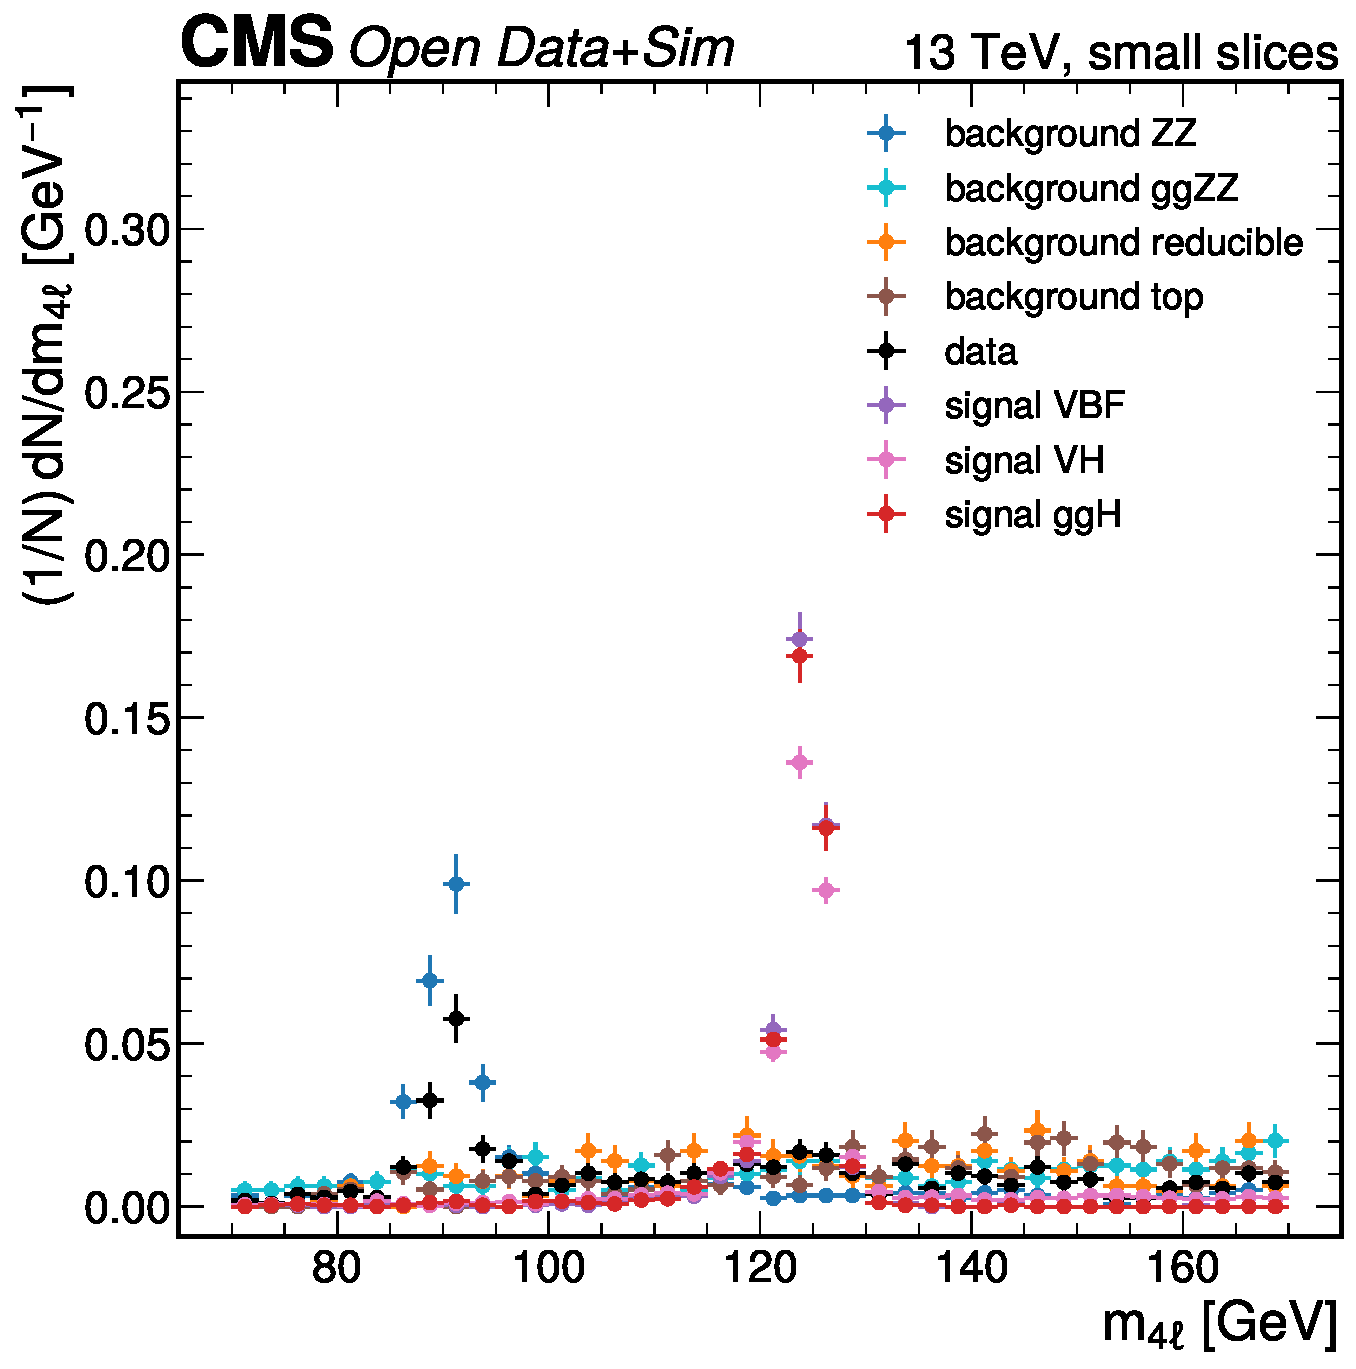
\includegraphics[width=0.92\linewidth,height=0.70\textheight,keepaspectratio]{figures/m4l_small_slice_shapes.pdf}
\caption{m\_\{4ell\} [GeV] small-slice shape comparison. The distributions use at most 1000 entries per primary ROOT file and are area-normalized only for Phase 1 shape reconnaissance, not for yield validation. Large differences here flag candidate variables for Phase 2/3 data-MC quality checks rather than final selection conclusions.}
\label{fig:m4l-small-slice-shapes}
\end{figure}

\begin{figure}[p]
\centering
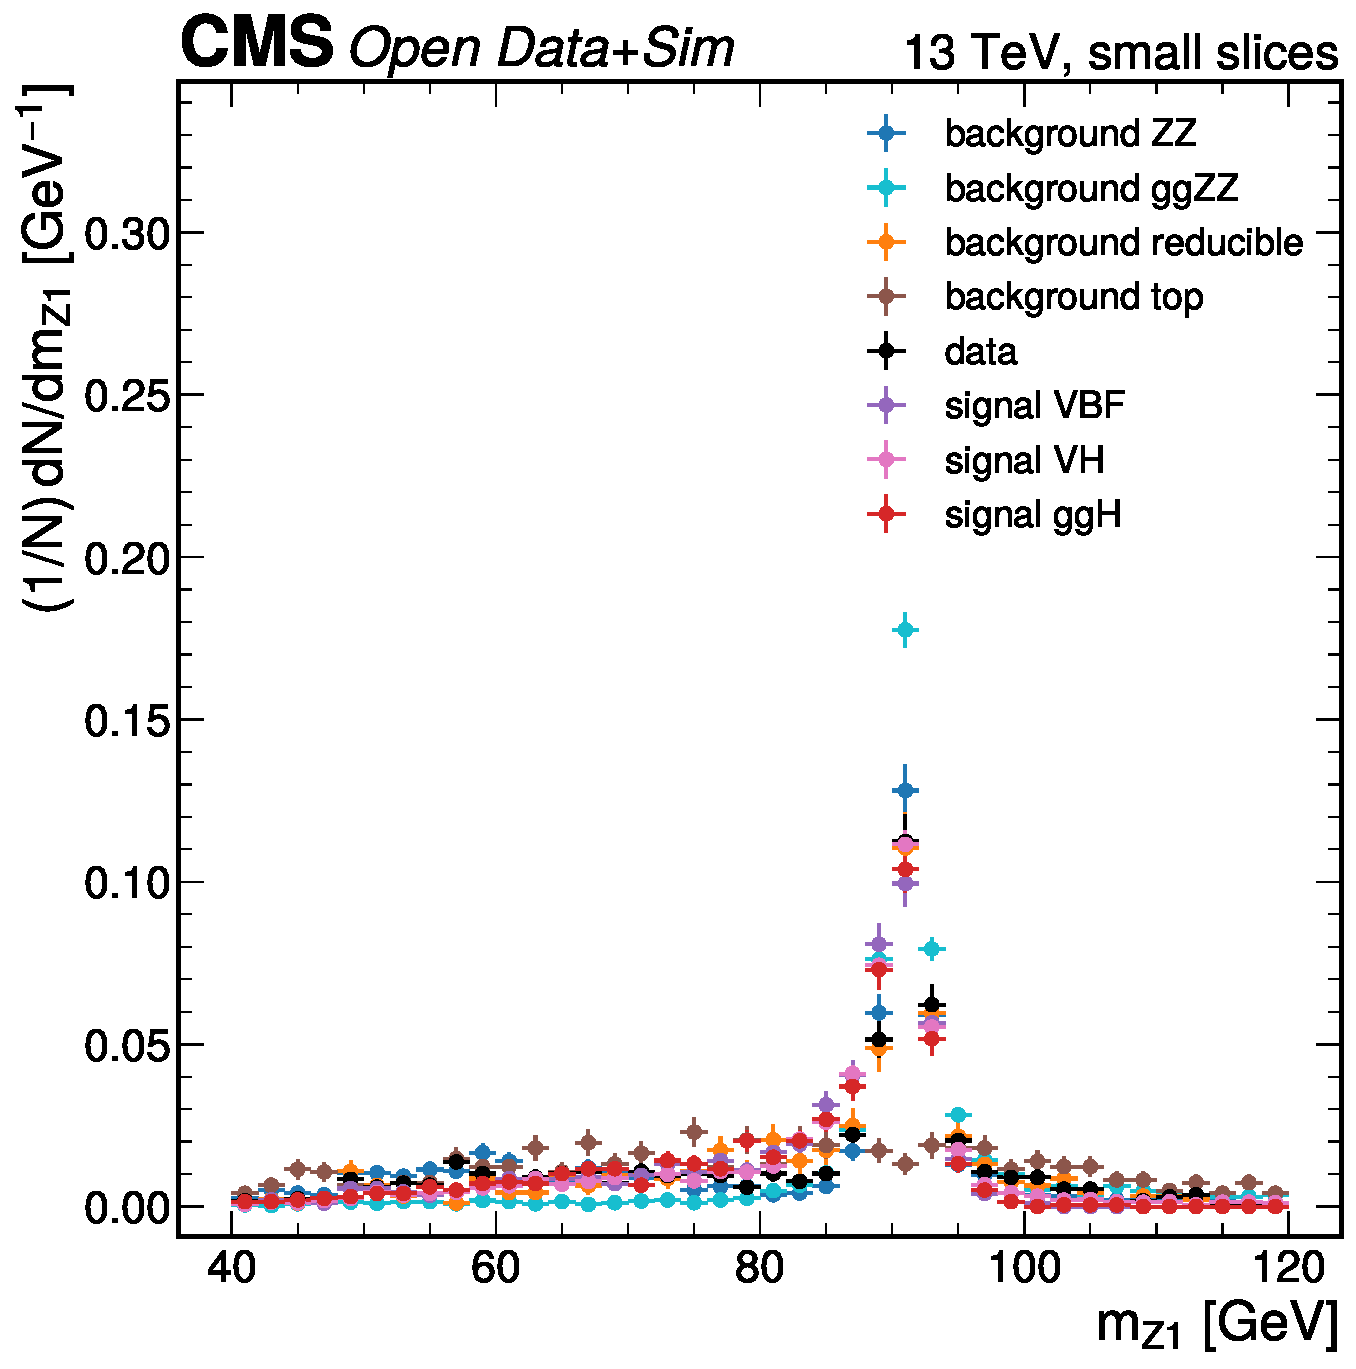
\includegraphics[width=0.92\linewidth,height=0.70\textheight,keepaspectratio]{figures/z1_mass_small_slice_shapes.pdf}
\caption{m\_\{Z1\} [GeV] small-slice shape comparison. The distributions use at most 1000 entries per primary ROOT file and are area-normalized only for Phase 1 shape reconnaissance, not for yield validation. Large differences here flag candidate variables for Phase 2/3 data-MC quality checks rather than final selection conclusions.}
\label{fig:z1-mass-small-slice-shapes}
\end{figure}

\begin{figure}[p]
\centering
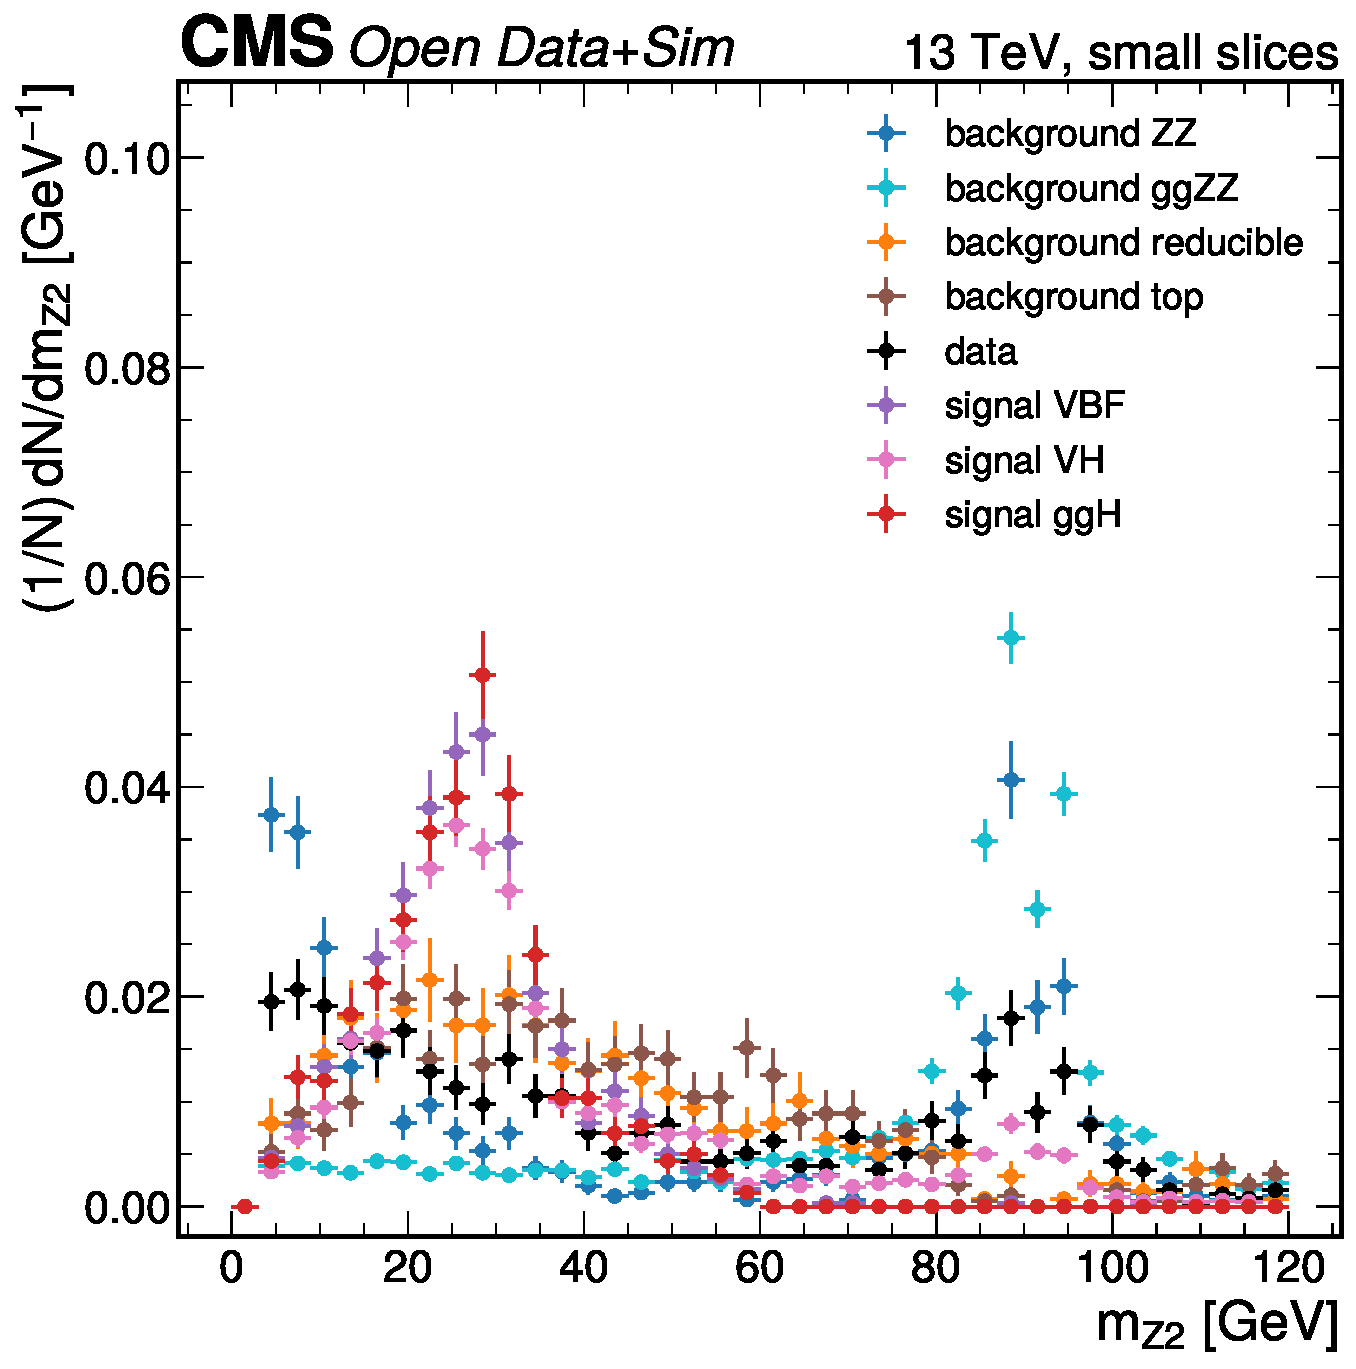
\includegraphics[width=0.92\linewidth,height=0.70\textheight,keepaspectratio]{figures/z2_mass_small_slice_shapes.pdf}
\caption{m\_\{Z2\} [GeV] small-slice shape comparison. The distributions use at most 1000 entries per primary ROOT file and are area-normalized only for Phase 1 shape reconnaissance, not for yield validation. Large differences here flag candidate variables for Phase 2/3 data-MC quality checks rather than final selection conclusions.}
\label{fig:z2-mass-small-slice-shapes}
\end{figure}

\begin{figure}[p]
\centering
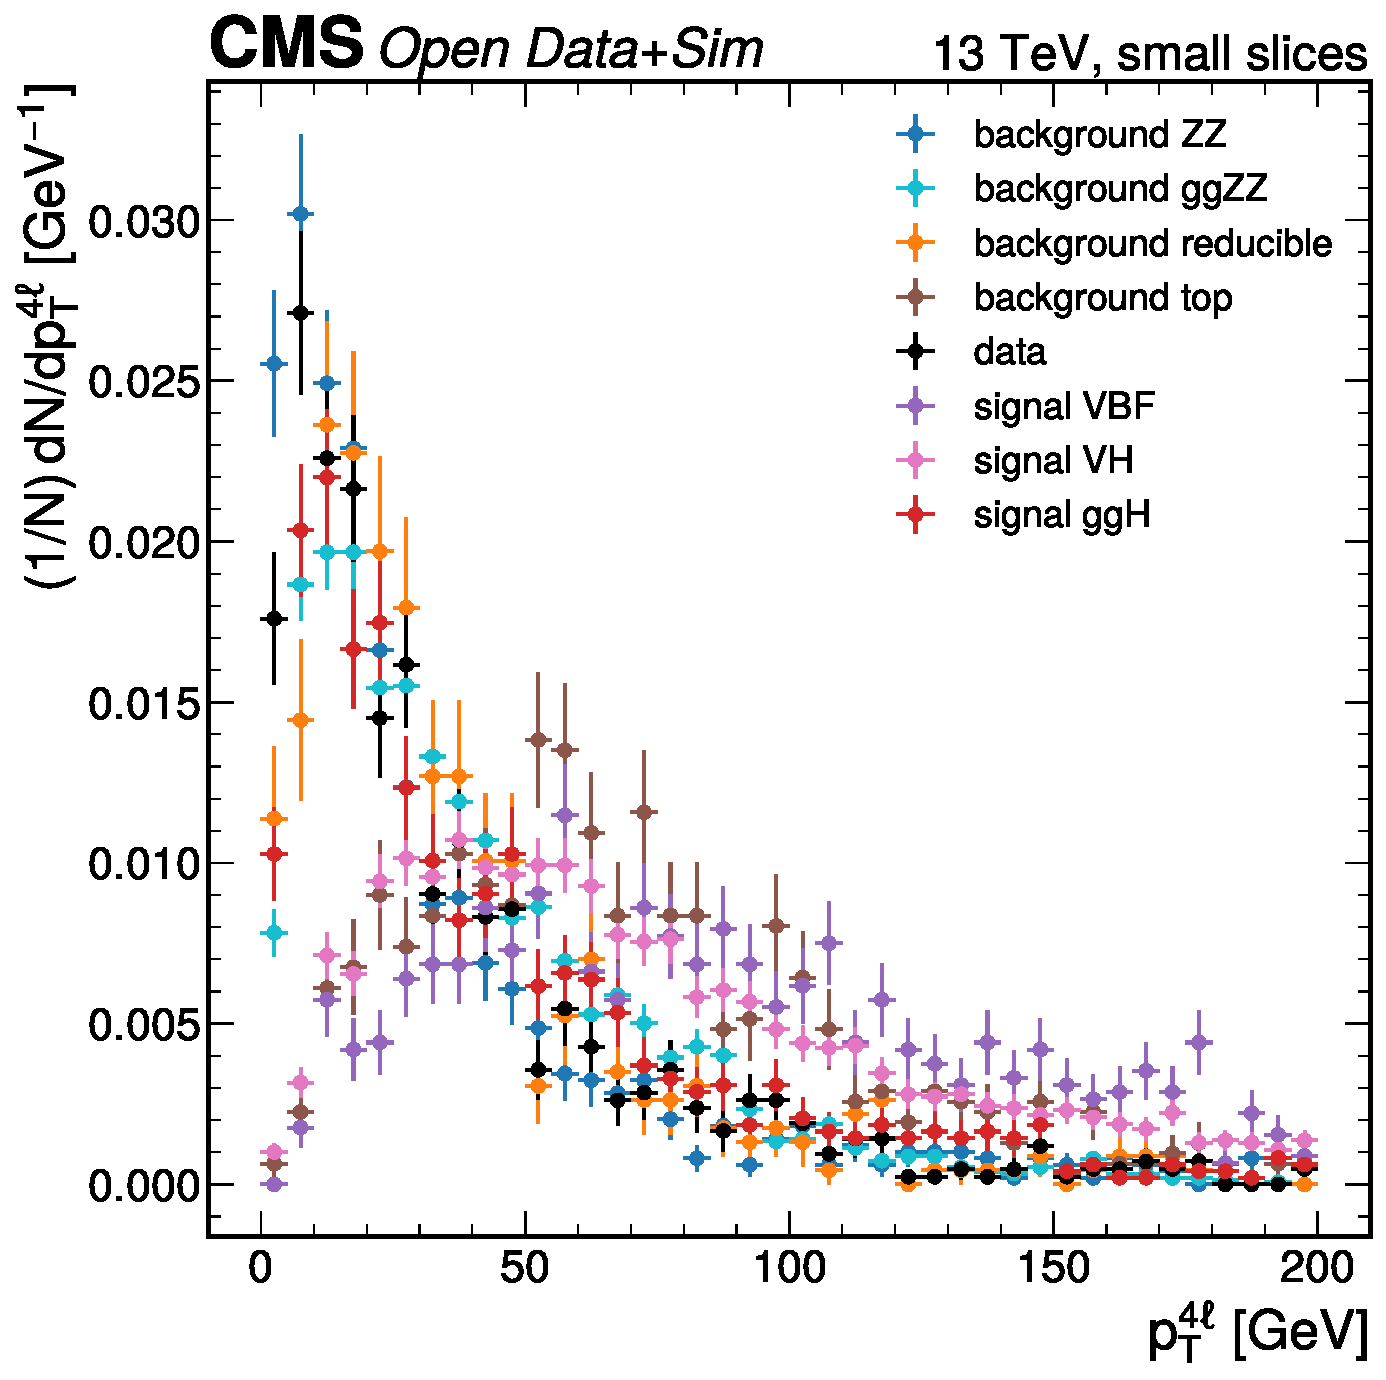
\includegraphics[width=0.92\linewidth,height=0.70\textheight,keepaspectratio]{figures/pt4l_small_slice_shapes.pdf}
\caption{p\_T\textasciicircum{}\{4ell\} [GeV] small-slice shape comparison. The distributions use at most 1000 entries per primary ROOT file and are area-normalized only for Phase 1 shape reconnaissance, not for yield validation. Large differences here flag candidate variables for Phase 2/3 data-MC quality checks rather than final selection conclusions.}
\label{fig:pt4l-small-slice-shapes}
\end{figure}

\begin{figure}[p]
\centering
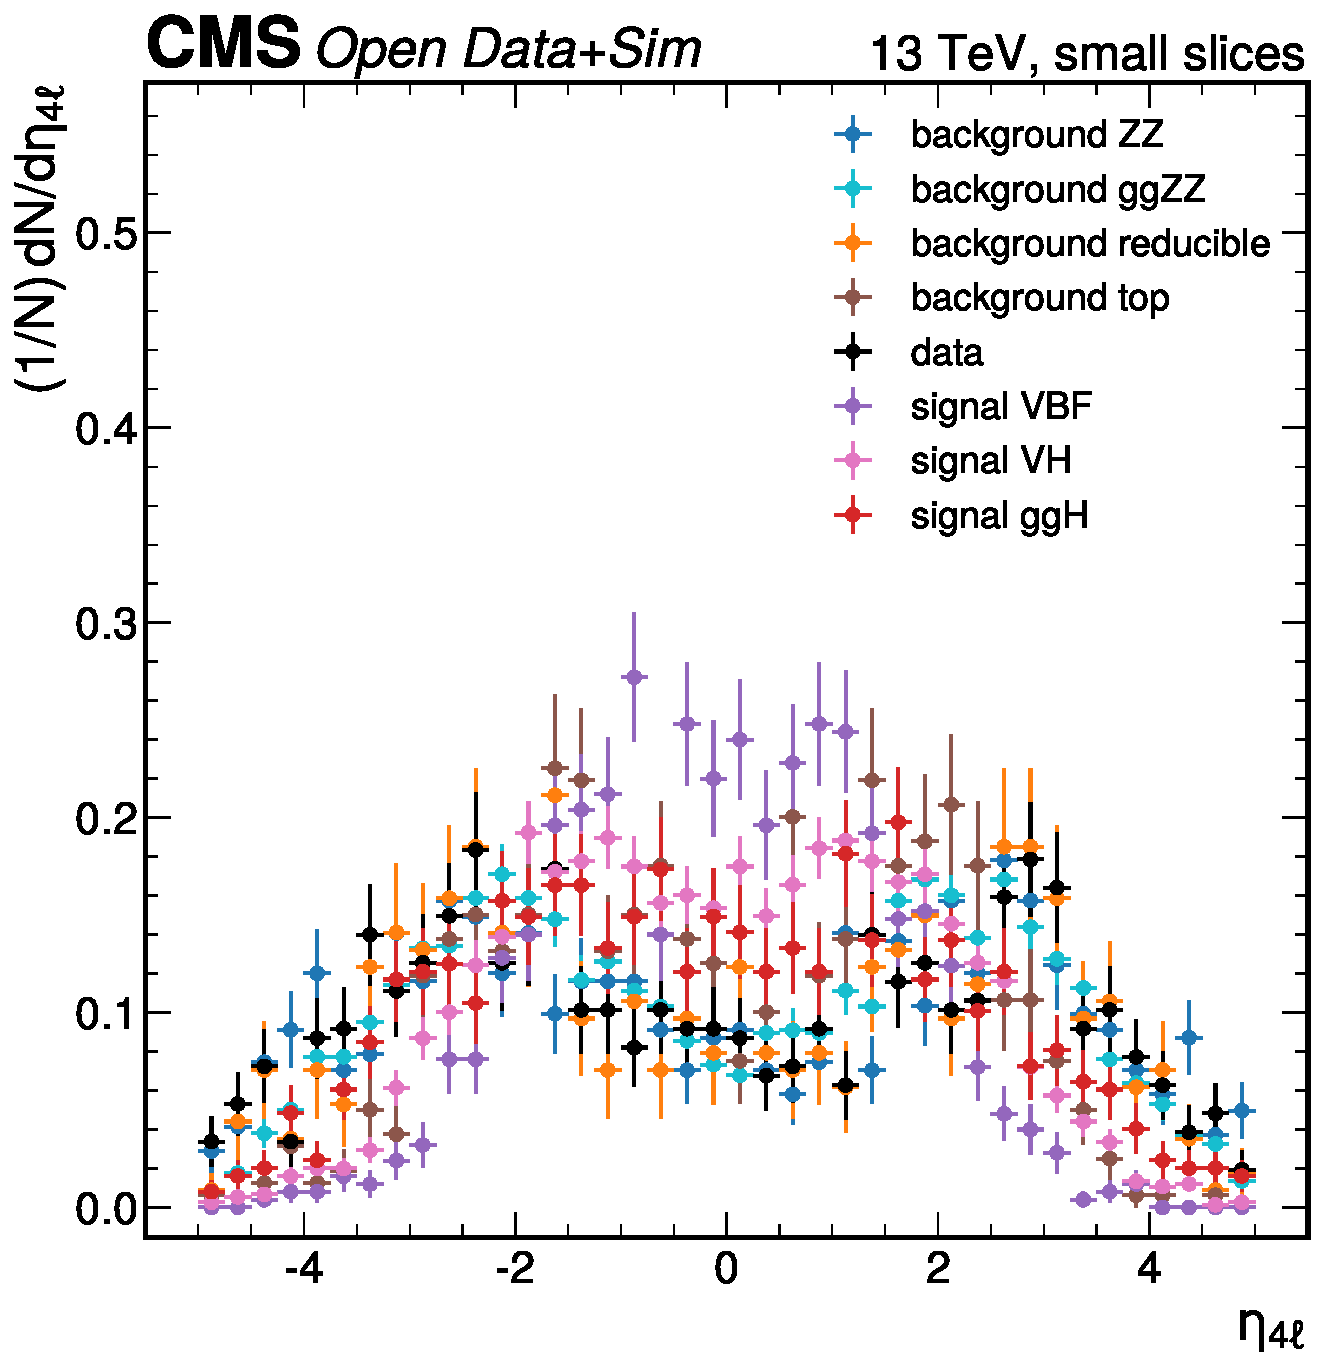
\includegraphics[width=0.92\linewidth,height=0.70\textheight,keepaspectratio]{figures/eta4l_small_slice_shapes.pdf}
\caption{eta\_\{4ell\} small-slice shape comparison. The distributions use at most 1000 entries per primary ROOT file and are area-normalized only for Phase 1 shape reconnaissance, not for yield validation. Large differences here flag candidate variables for Phase 2/3 data-MC quality checks rather than final selection conclusions.}
\label{fig:eta4l-small-slice-shapes}
\end{figure}

\begin{figure}[p]
\centering
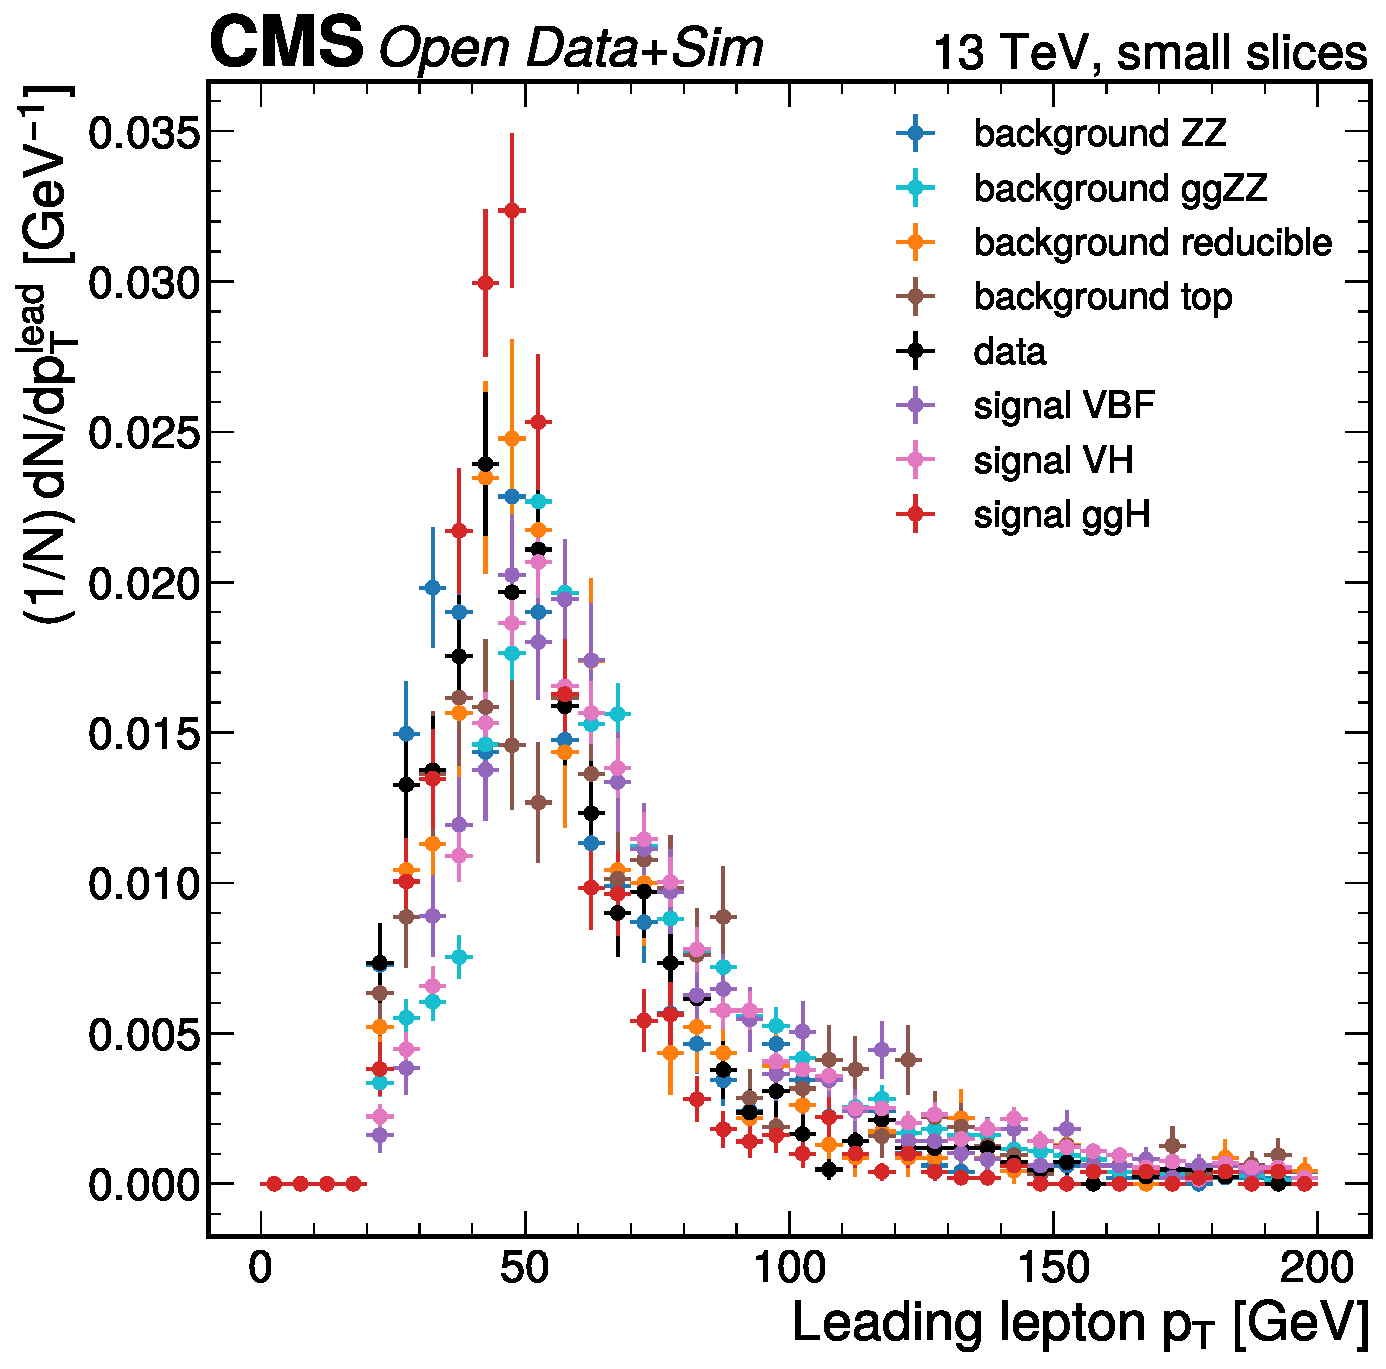
\includegraphics[width=0.92\linewidth,height=0.70\textheight,keepaspectratio]{figures/leading_lepton_pt_small_slice_shapes.pdf}
\caption{Leading lepton p\_T [GeV] small-slice shape comparison. The distributions use at most 1000 entries per primary ROOT file and are area-normalized only for Phase 1 shape reconnaissance, not for yield validation. Large differences here flag candidate variables for Phase 2/3 data-MC quality checks rather than final selection conclusions.}
\label{fig:leading-lepton-pt-small-slice-shapes}
\end{figure}

\begin{figure}[p]
\centering
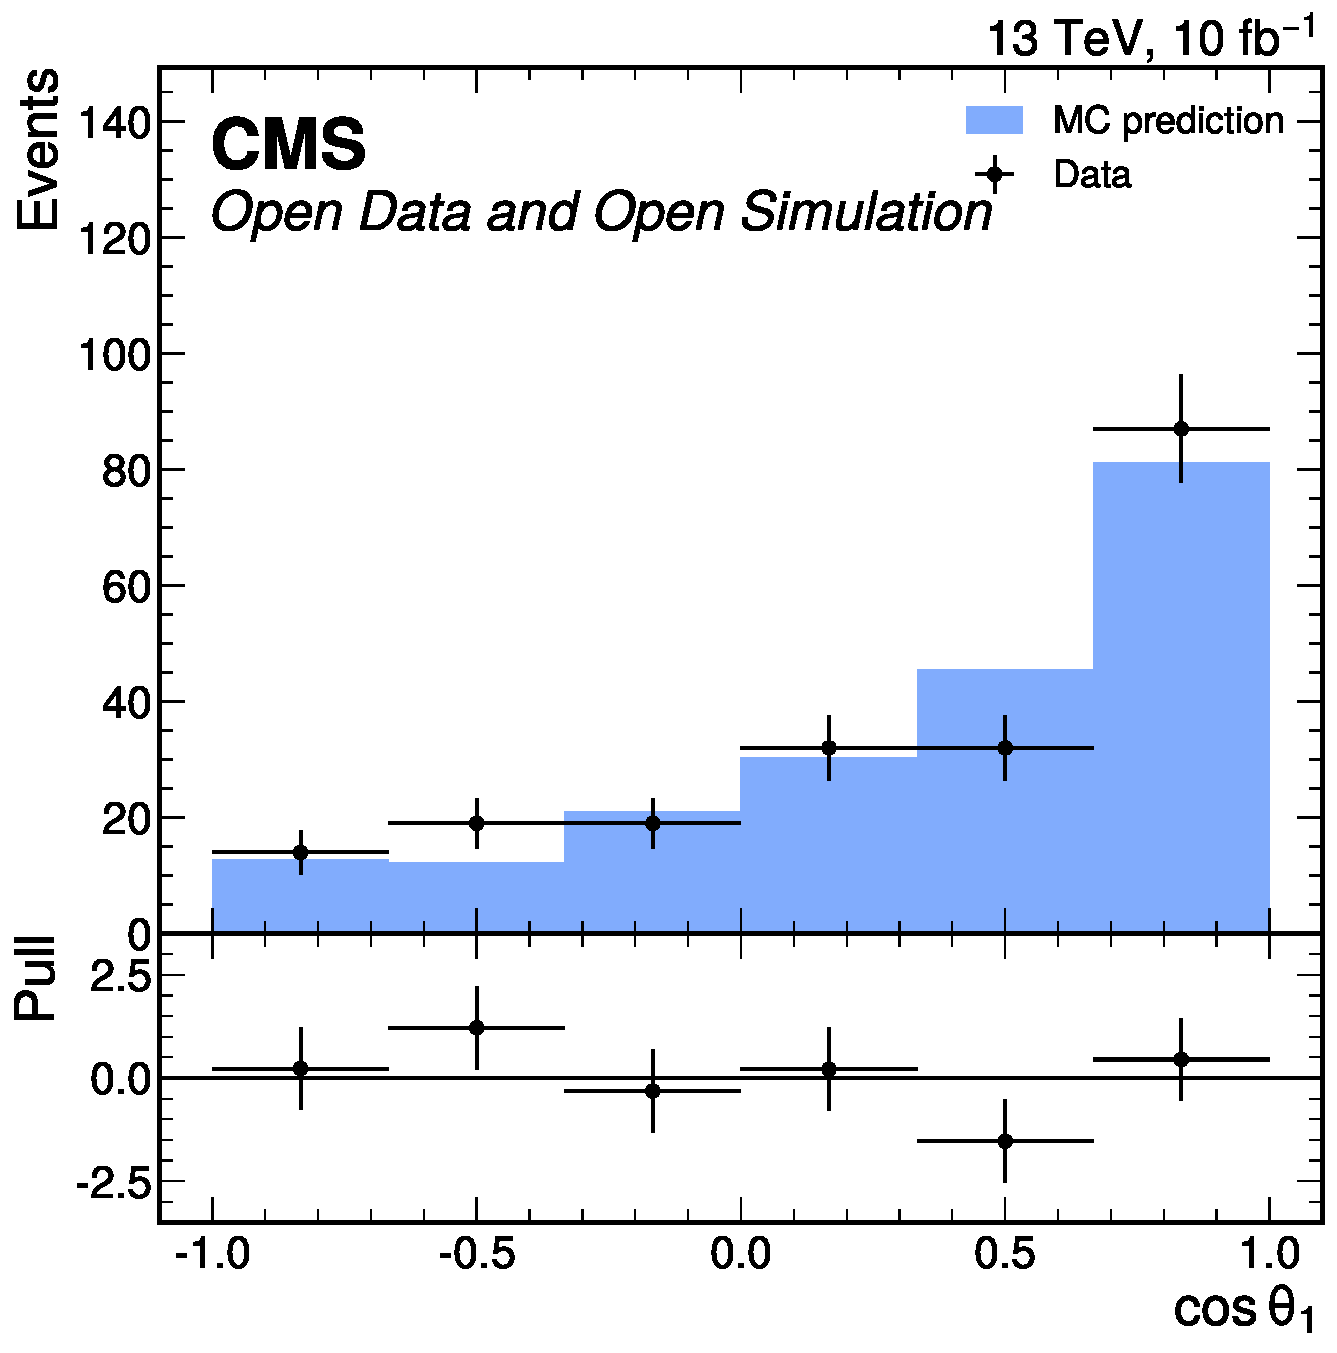
\includegraphics[width=0.92\linewidth,height=0.70\textheight,keepaspectratio]{figures/input_validation_cos_theta1.pdf}
\caption{costheta\_1 input-validation distribution in the broad $70 \le m_{4\ell} \le 170$ GeV window. The D7 shape gate fails with chi2/ndf = 1.60 and p = 0.156; this comparison is used only to decide classifier-input eligibility, not to normalize fit templates.}
\label{fig:input-validation-cos-theta1}
\end{figure}

\begin{figure}[p]
\centering
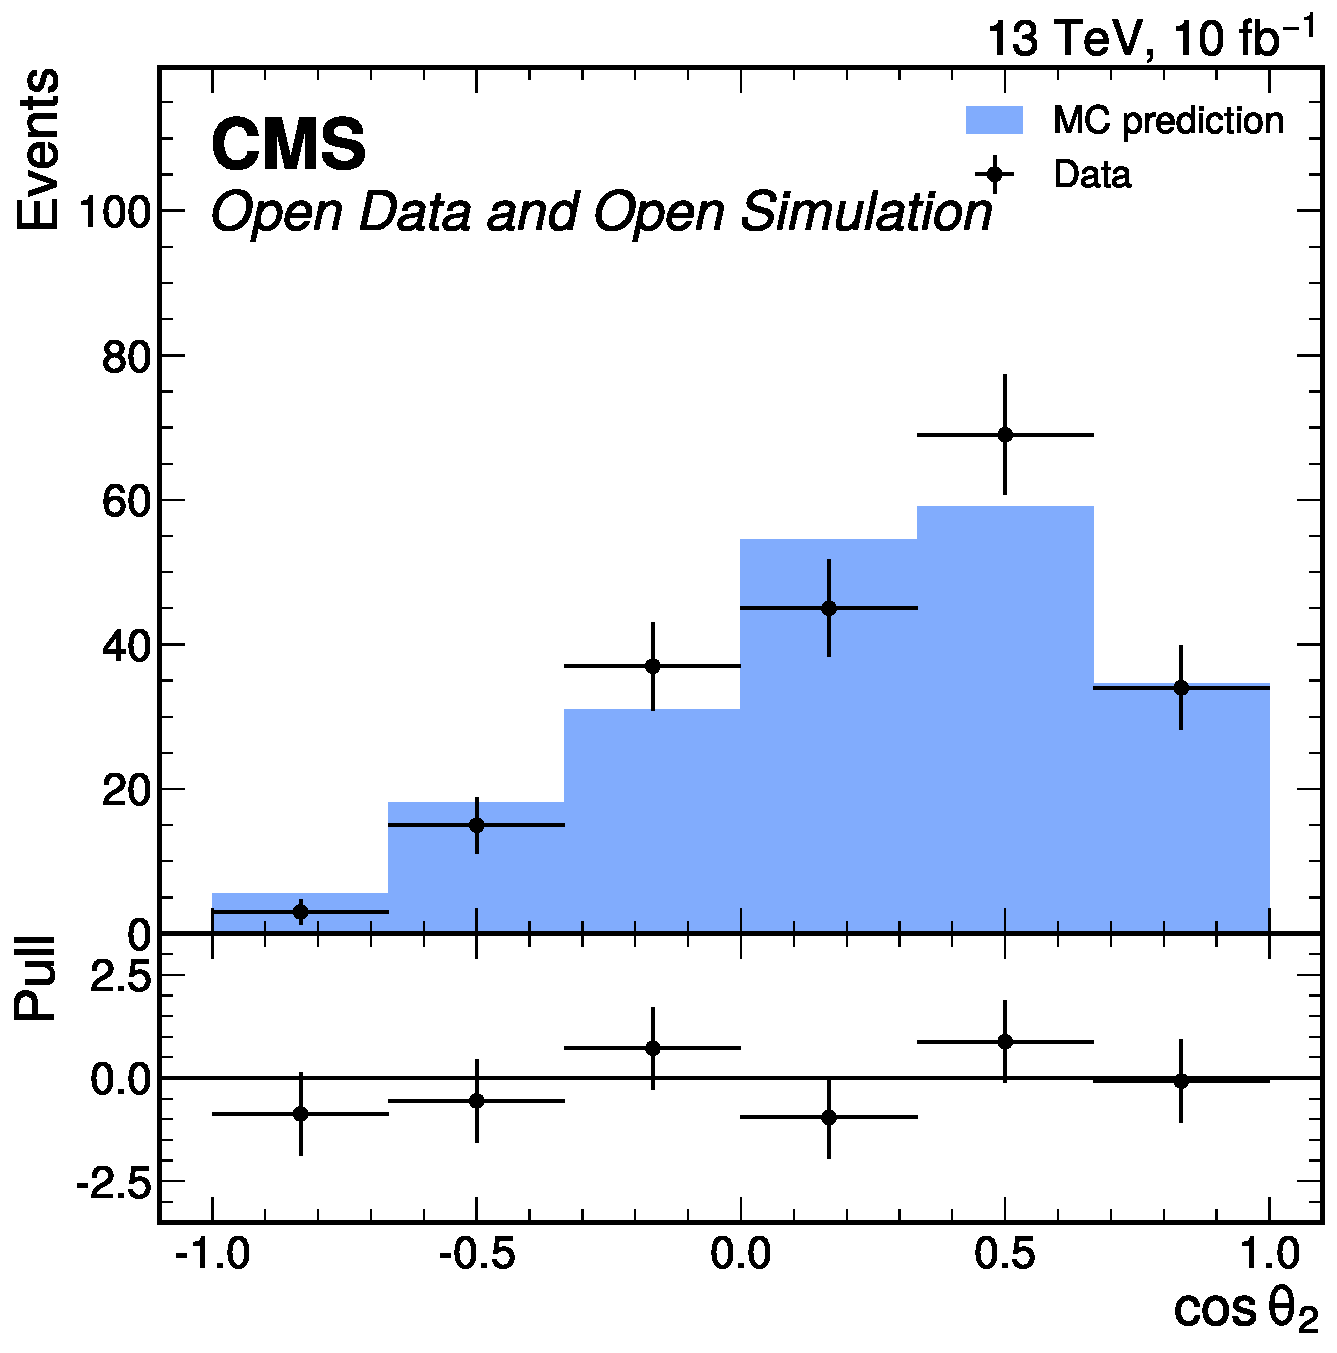
\includegraphics[width=0.92\linewidth,height=0.70\textheight,keepaspectratio]{figures/input_validation_cos_theta2.pdf}
\caption{costheta\_2 input-validation distribution in the broad $70 \le m_{4\ell} \le 170$ GeV window. The D7 shape gate fails with chi2/ndf = 1.29 and p = 0.265; this comparison is used only to decide classifier-input eligibility, not to normalize fit templates.}
\label{fig:input-validation-cos-theta2}
\end{figure}

\begin{figure}[p]
\centering
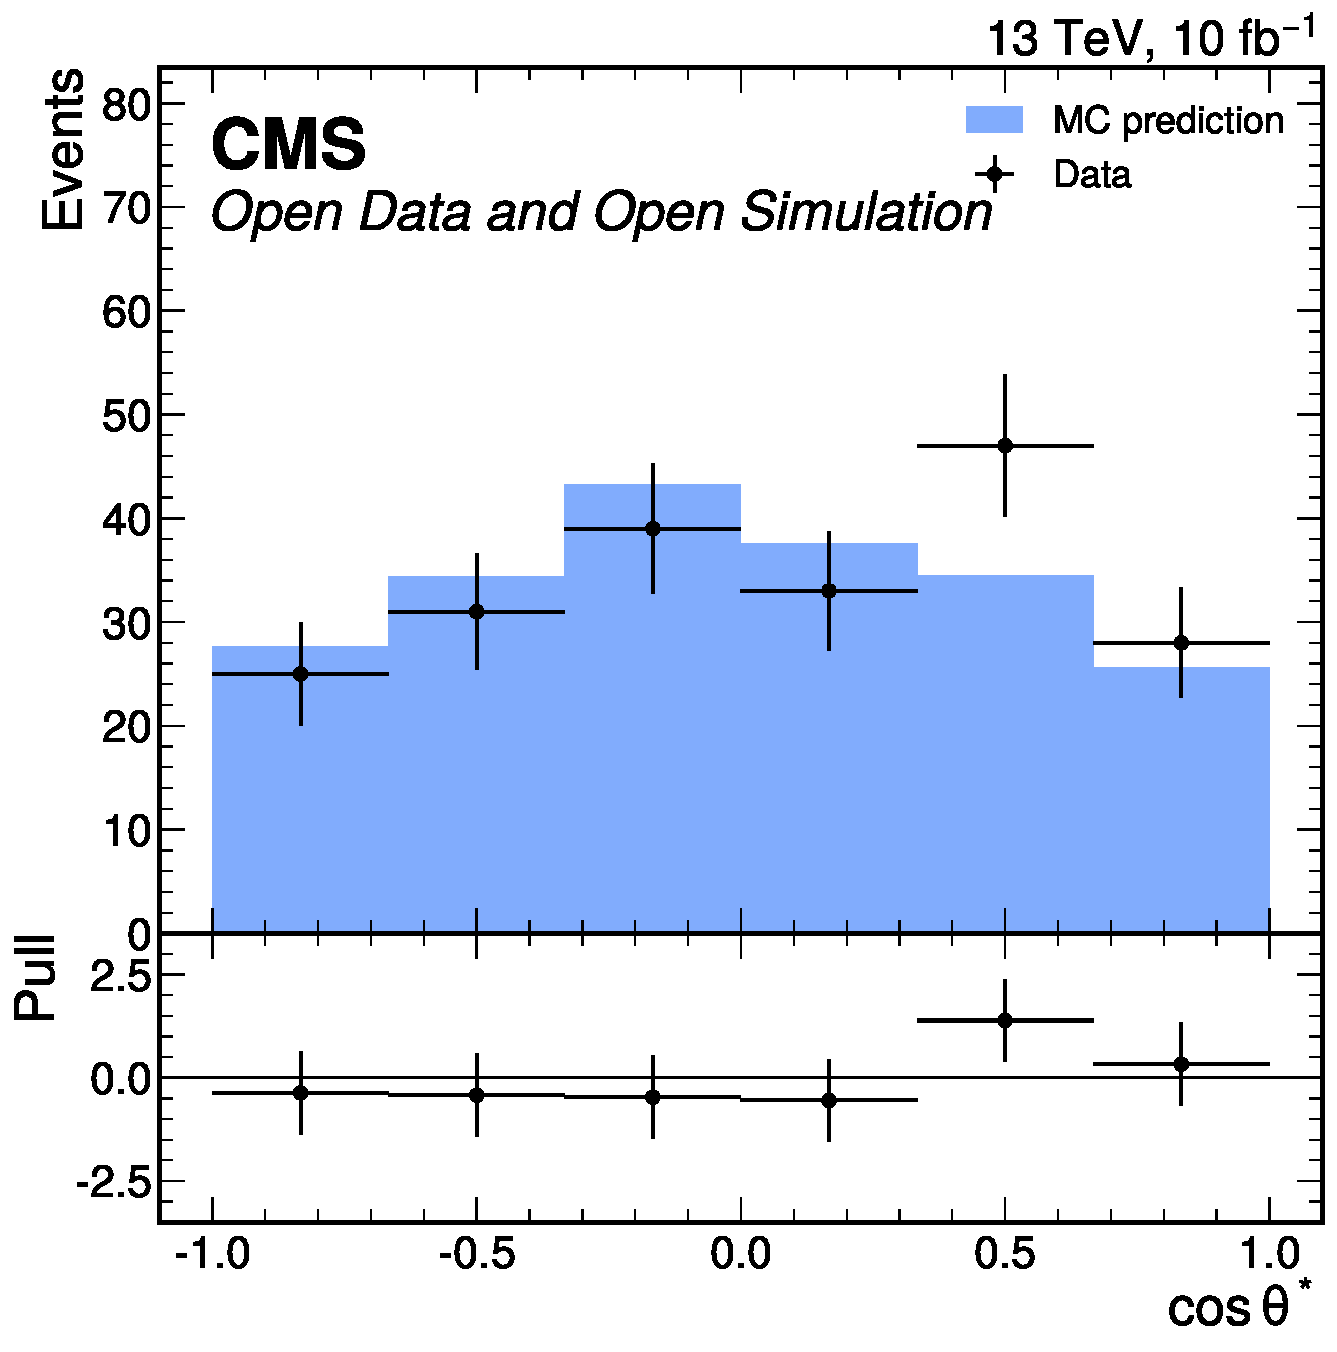
\includegraphics[width=0.92\linewidth,height=0.70\textheight,keepaspectratio]{figures/input_validation_cos_theta_star.pdf}
\caption{costheta\textasciicircum{}* input-validation distribution in the broad $70 \le m_{4\ell} \le 170$ GeV window. The D7 shape gate fails with chi2/ndf = 1.01 and p = 0.412; this comparison is used only to decide classifier-input eligibility, not to normalize fit templates.}
\label{fig:input-validation-cos-theta-star}
\end{figure}

\begin{figure}[p]
\centering
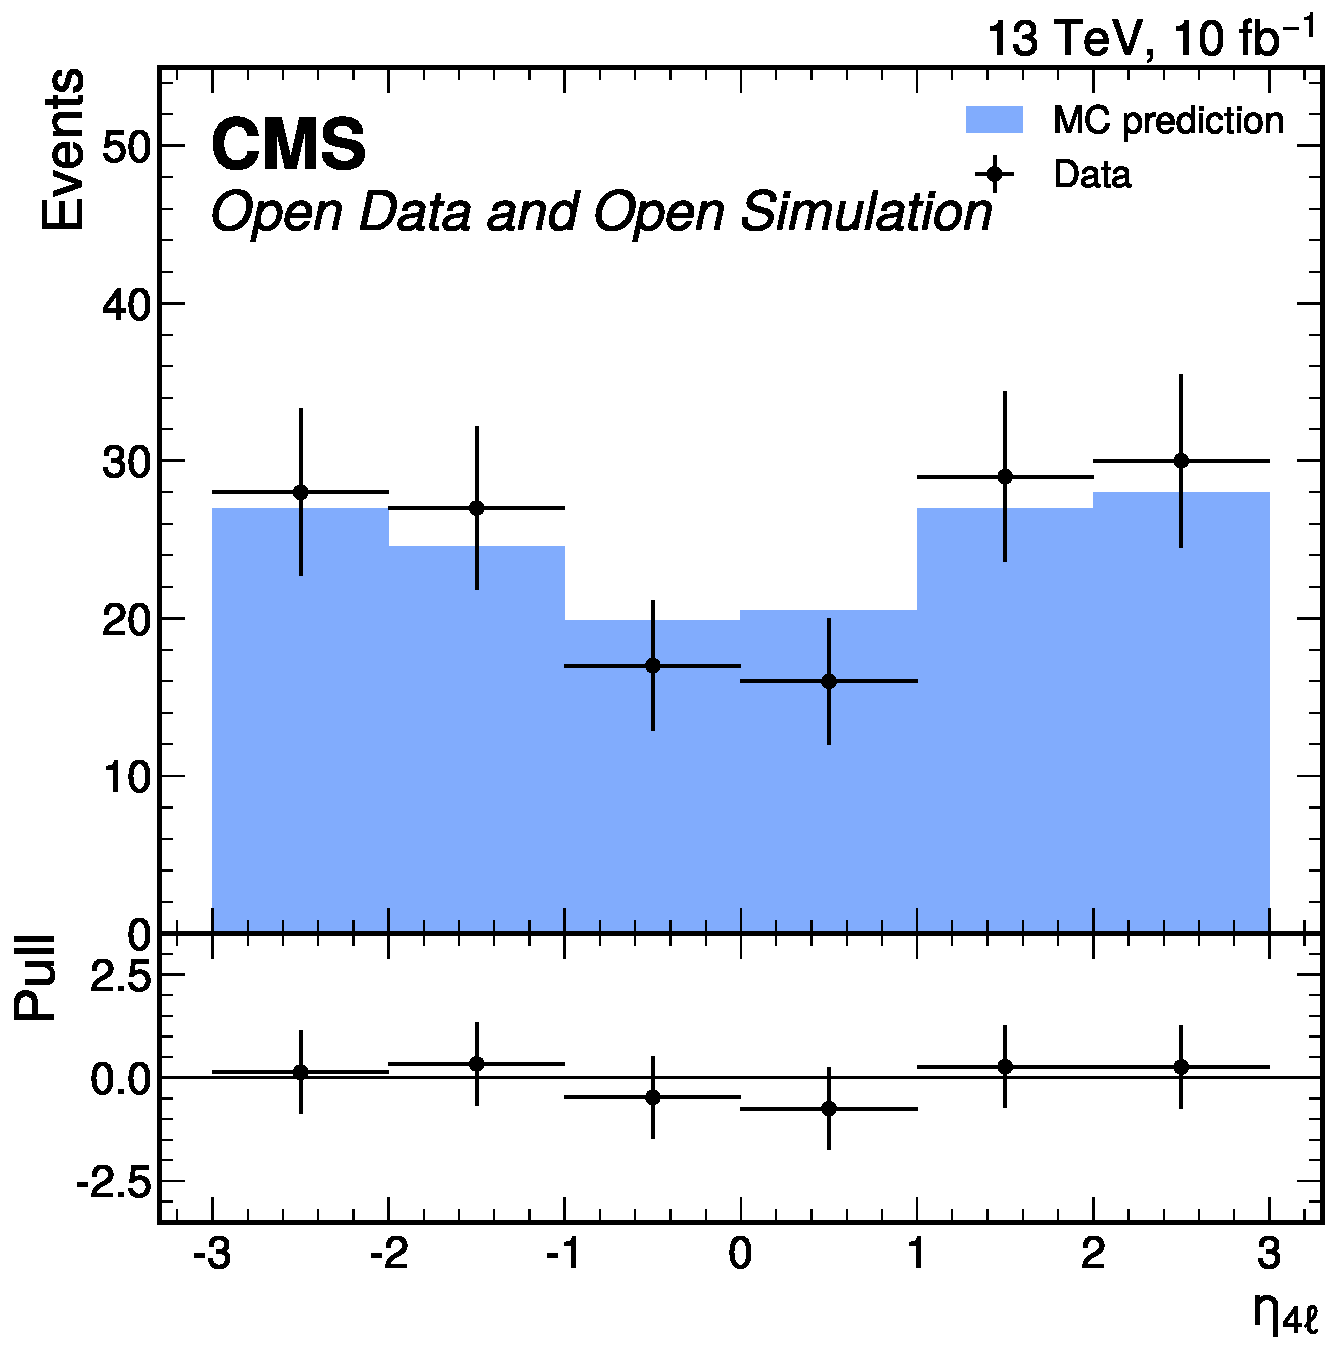
\includegraphics[width=0.92\linewidth,height=0.70\textheight,keepaspectratio]{figures/input_validation_eta4l.pdf}
\caption{eta\_\{4ell\} input-validation distribution in the broad $70 \le m_{4\ell} \le 170$ GeV window. The D7 shape gate fails with chi2/ndf = 0.404 and p = 0.846; this comparison is used only to decide classifier-input eligibility, not to normalize fit templates.}
\label{fig:input-validation-eta4l}
\end{figure}

\begin{figure}[p]
\centering
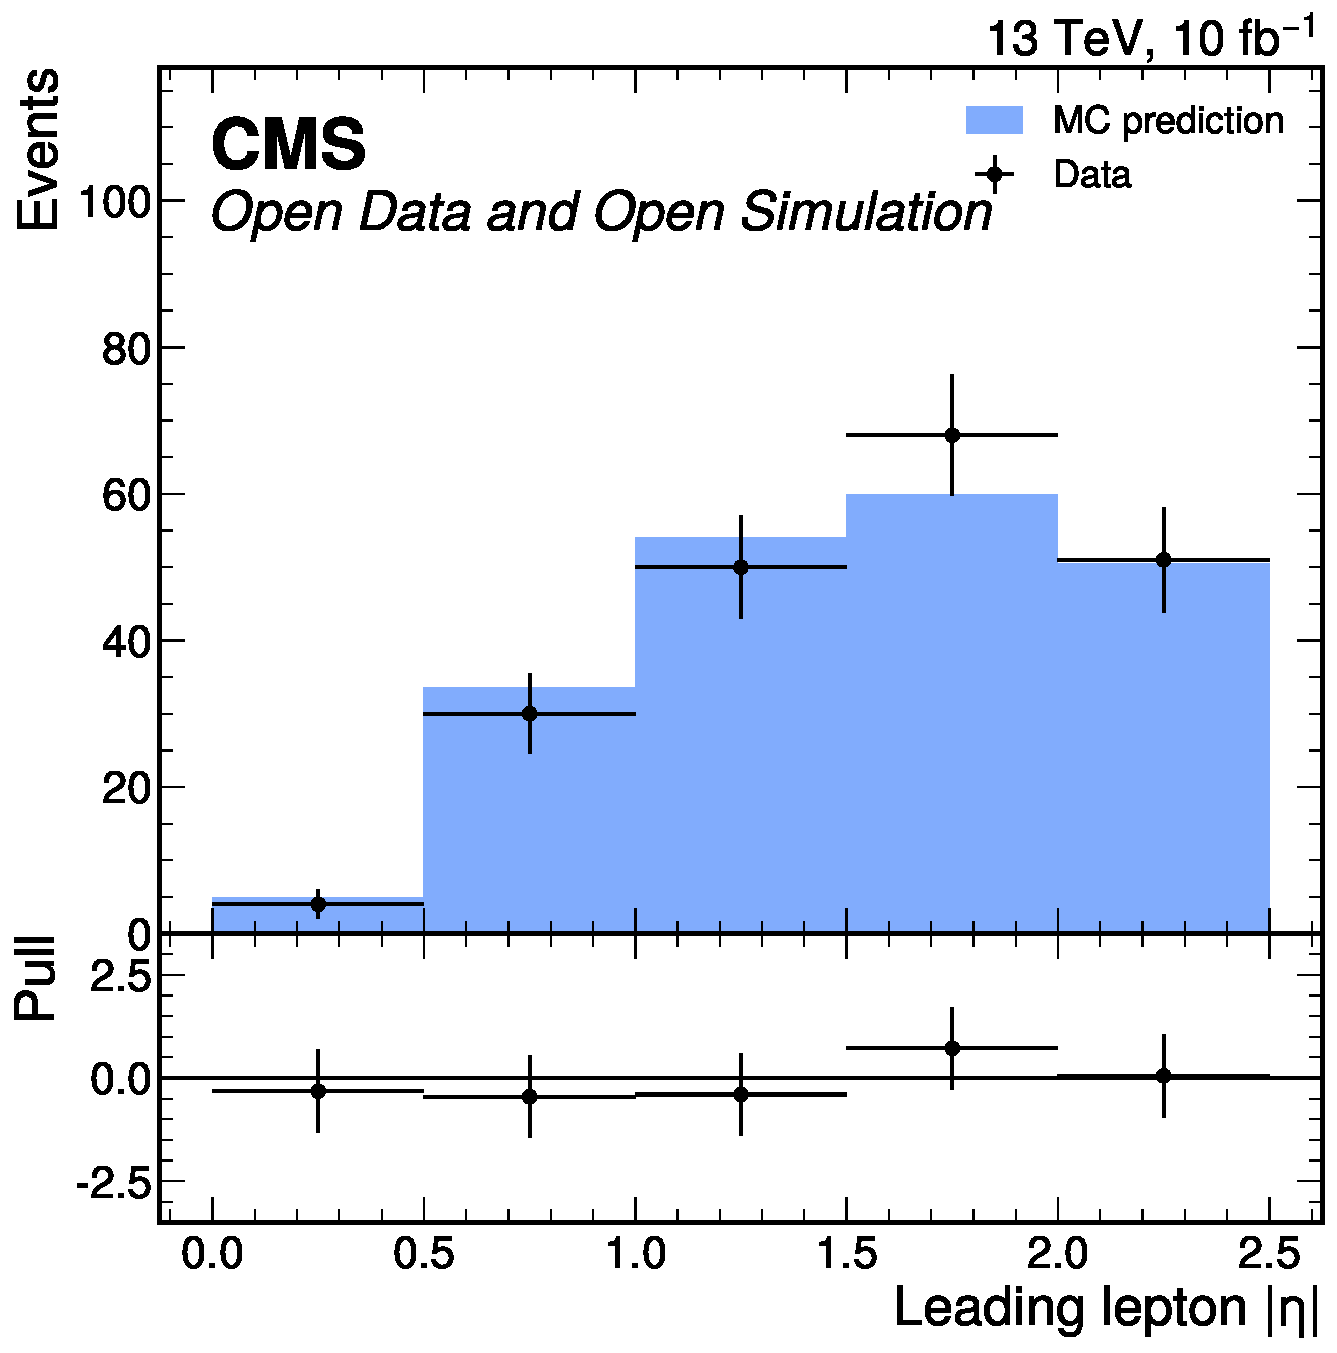
\includegraphics[width=0.92\linewidth,height=0.70\textheight,keepaspectratio]{figures/input_validation_lead_abs_eta.pdf}
\caption{Leading lepton |eta| input-validation distribution in the broad $70 \le m_{4\ell} \le 170$ GeV window. The D7 shape gate passes with chi2/ndf = 0.473 and p = 0.755; this comparison is used only to decide classifier-input eligibility, not to normalize fit templates.}
\label{fig:input-validation-lead-abs-eta}
\end{figure}

\begin{figure}[p]
\centering
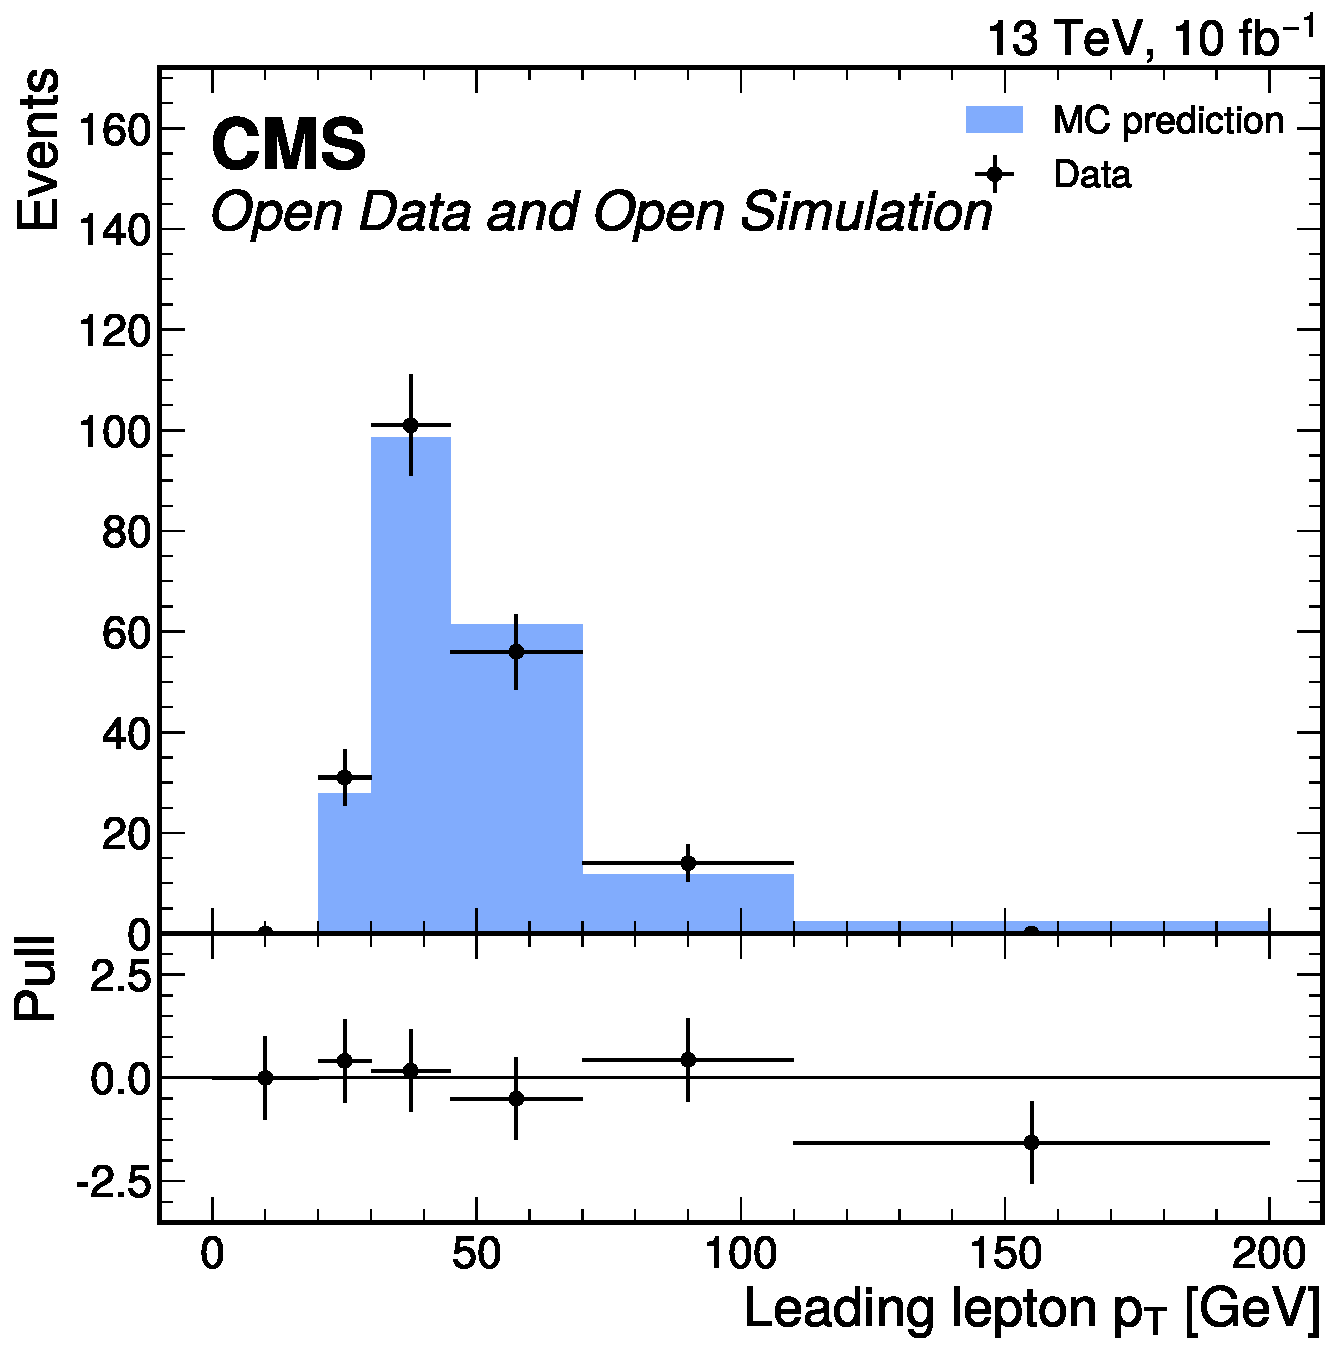
\includegraphics[width=0.92\linewidth,height=0.70\textheight,keepaspectratio]{figures/input_validation_lead_lepton_pt.pdf}
\caption{Leading lepton p\_T [GeV] input-validation distribution in the broad $70 \le m_{4\ell} \le 170$ GeV window. The D7 shape gate fails with chi2/ndf = 4.06 and p = 0.00273; this comparison is used only to decide classifier-input eligibility, not to normalize fit templates.}
\label{fig:input-validation-lead-lepton-pt}
\end{figure}

\begin{figure}[p]
\centering
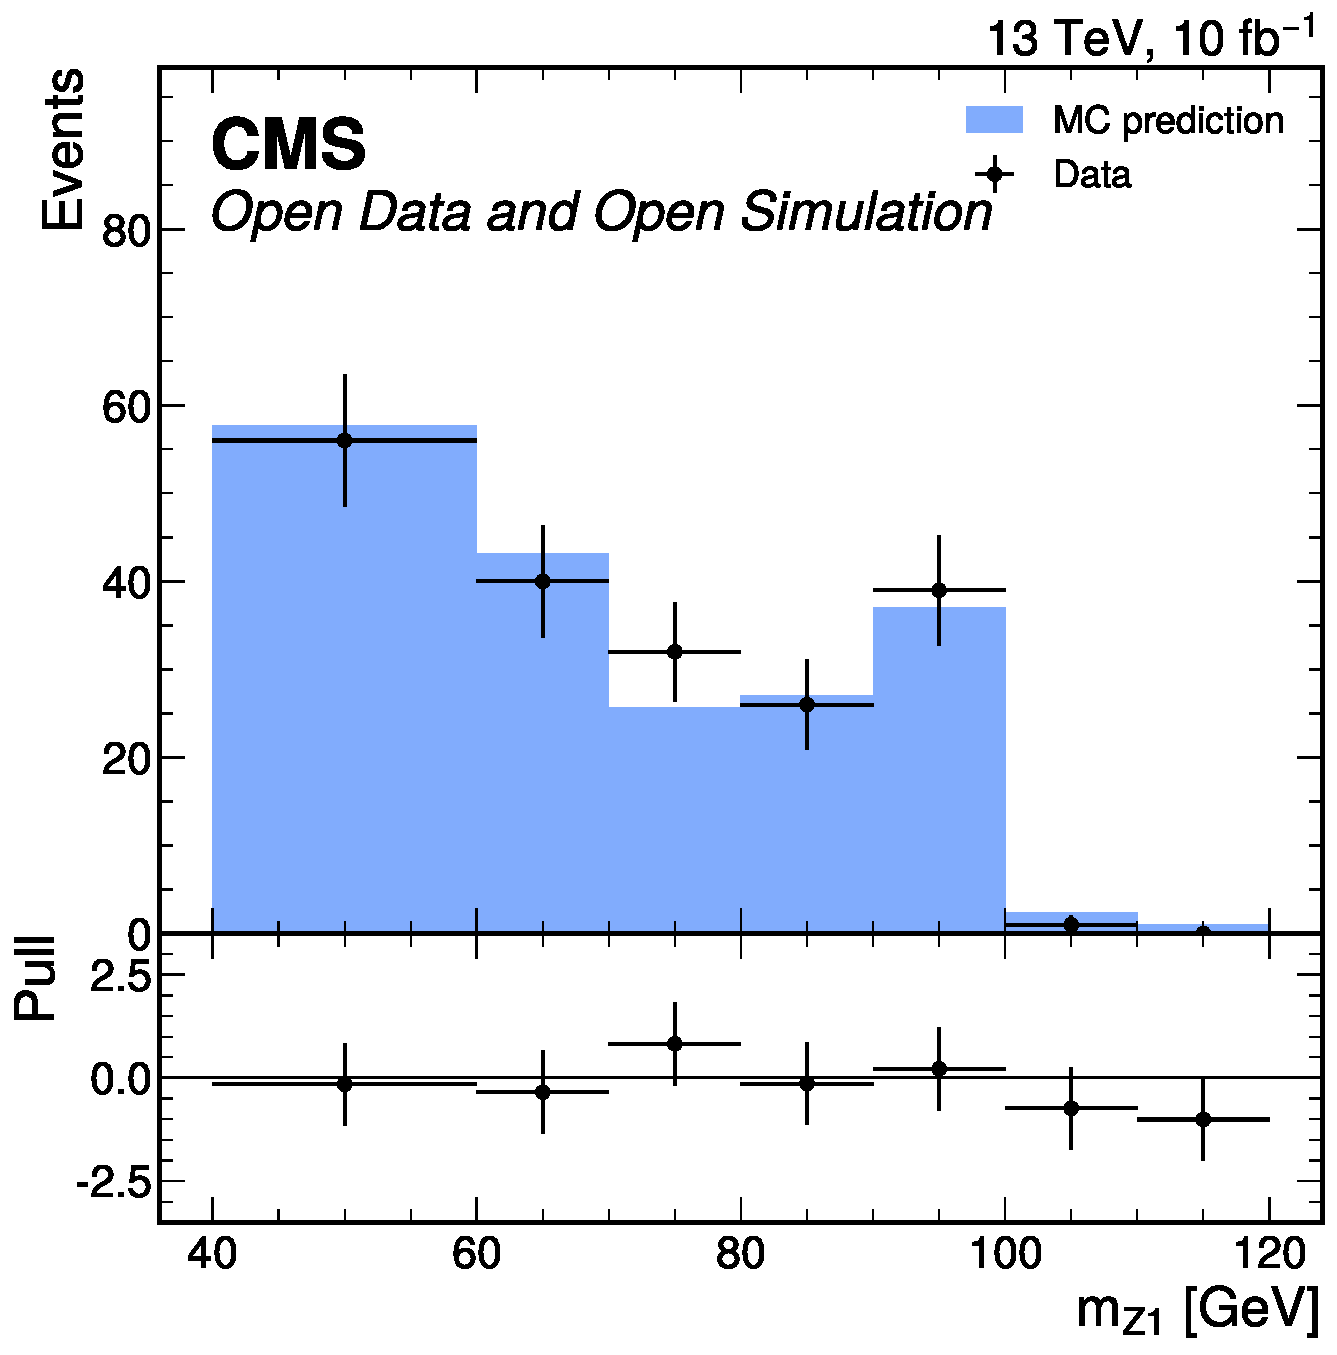
\includegraphics[width=0.92\linewidth,height=0.70\textheight,keepaspectratio]{figures/input_validation_mZ1.pdf}
\caption{m\_\{Z1\} [GeV] input-validation distribution in the broad $70 \le m_{4\ell} \le 170$ GeV window. The D7 shape gate fails with chi2/ndf = 122.06 and p = $6.22\times10^{-155}$; this comparison is used only to decide classifier-input eligibility, not to normalize fit templates.}
\label{fig:input-validation-mZ1}
\end{figure}

\begin{figure}[p]
\centering
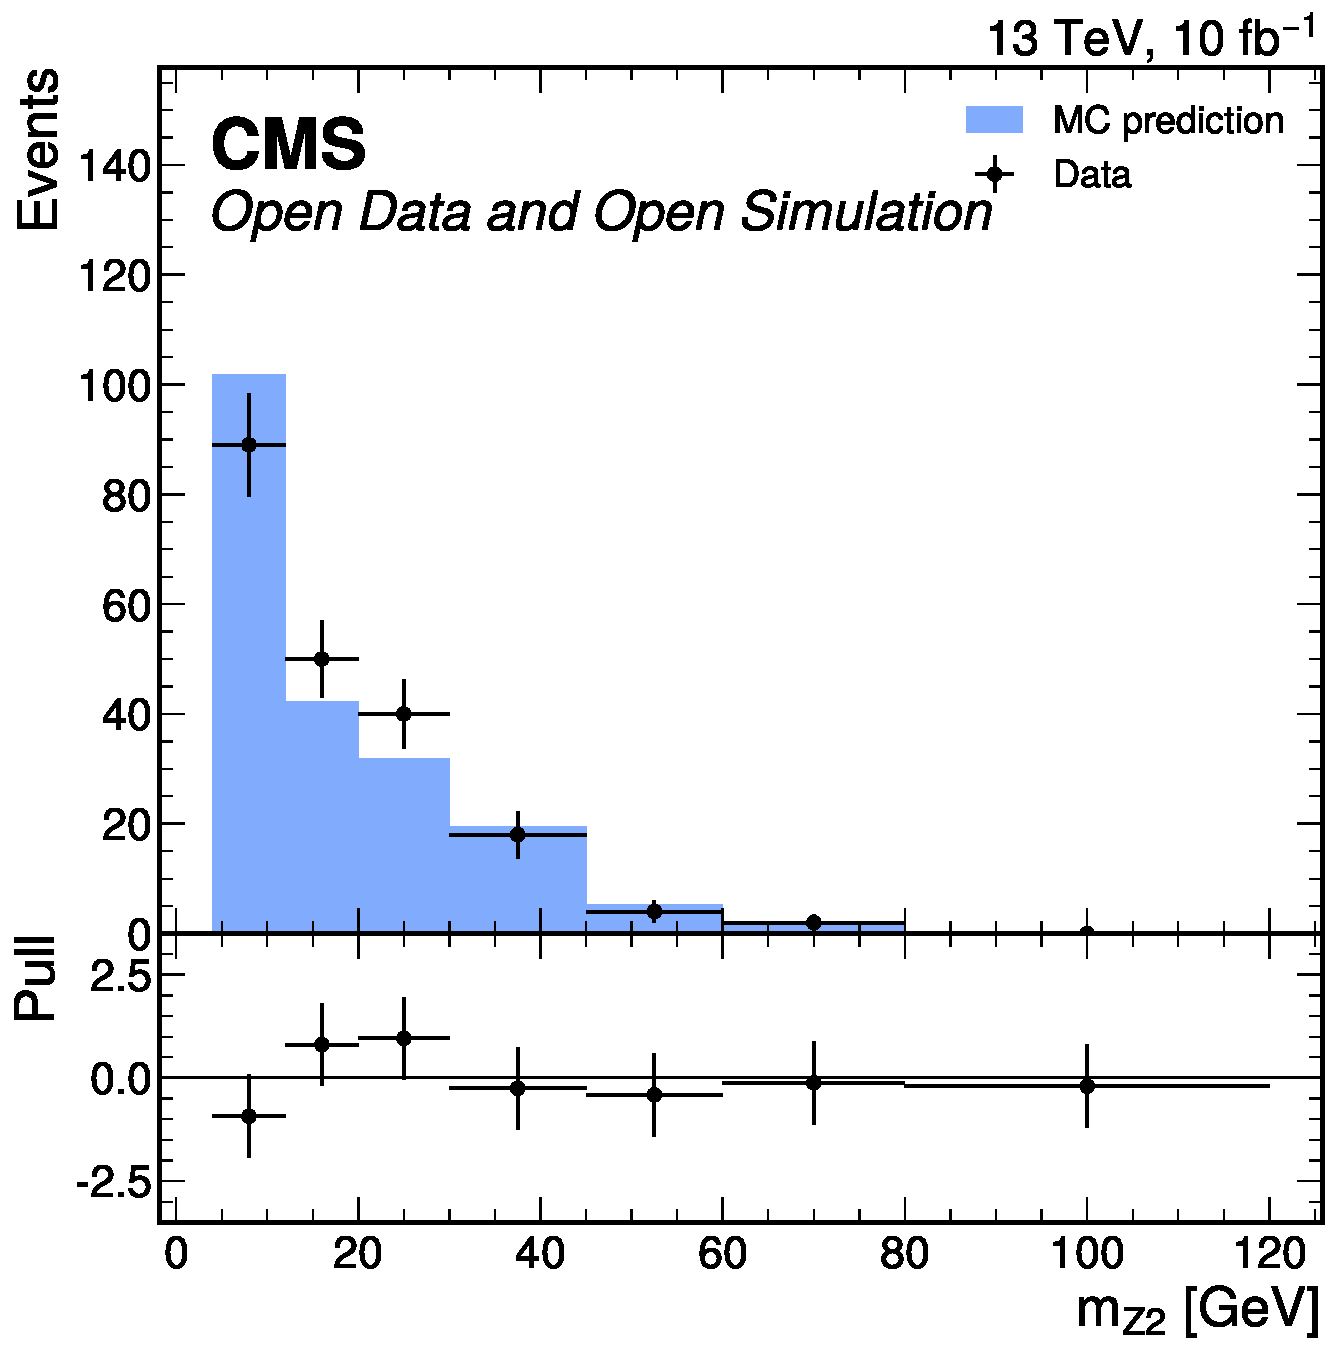
\includegraphics[width=0.92\linewidth,height=0.70\textheight,keepaspectratio]{figures/input_validation_mZ2.pdf}
\caption{m\_\{Z2\} [GeV] input-validation distribution in the broad $70 \le m_{4\ell} \le 170$ GeV window. The D7 shape gate fails with chi2/ndf = 32.08 and p = $7.49\times10^{-39}$; this comparison is used only to decide classifier-input eligibility, not to normalize fit templates.}
\label{fig:input-validation-mZ2}
\end{figure}

\begin{figure}[p]
\centering
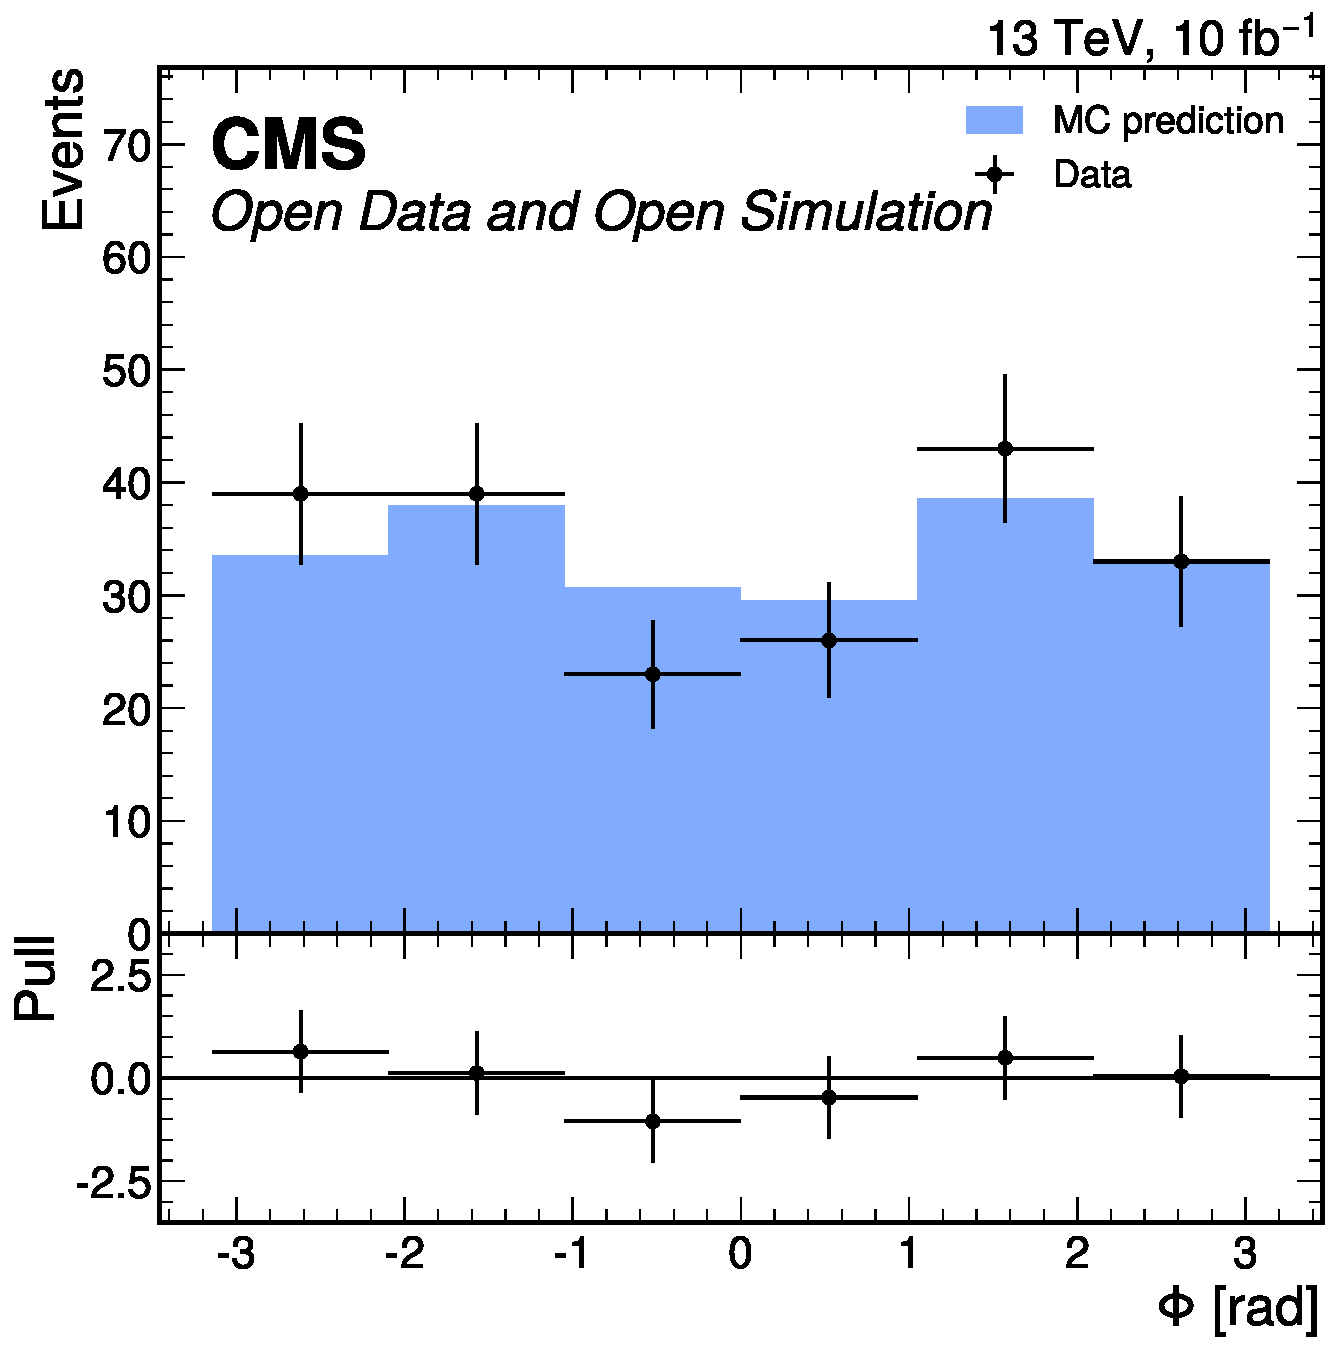
\includegraphics[width=0.92\linewidth,height=0.70\textheight,keepaspectratio]{figures/input_validation_phi.pdf}
\caption{Phi [rad] input-validation distribution in the broad $70 \le m_{4\ell} \le 170$ GeV window. The D7 shape gate fails with chi2/ndf = 0.780 and p = 0.564; this comparison is used only to decide classifier-input eligibility, not to normalize fit templates.}
\label{fig:input-validation-phi}
\end{figure}

\begin{figure}[p]
\centering
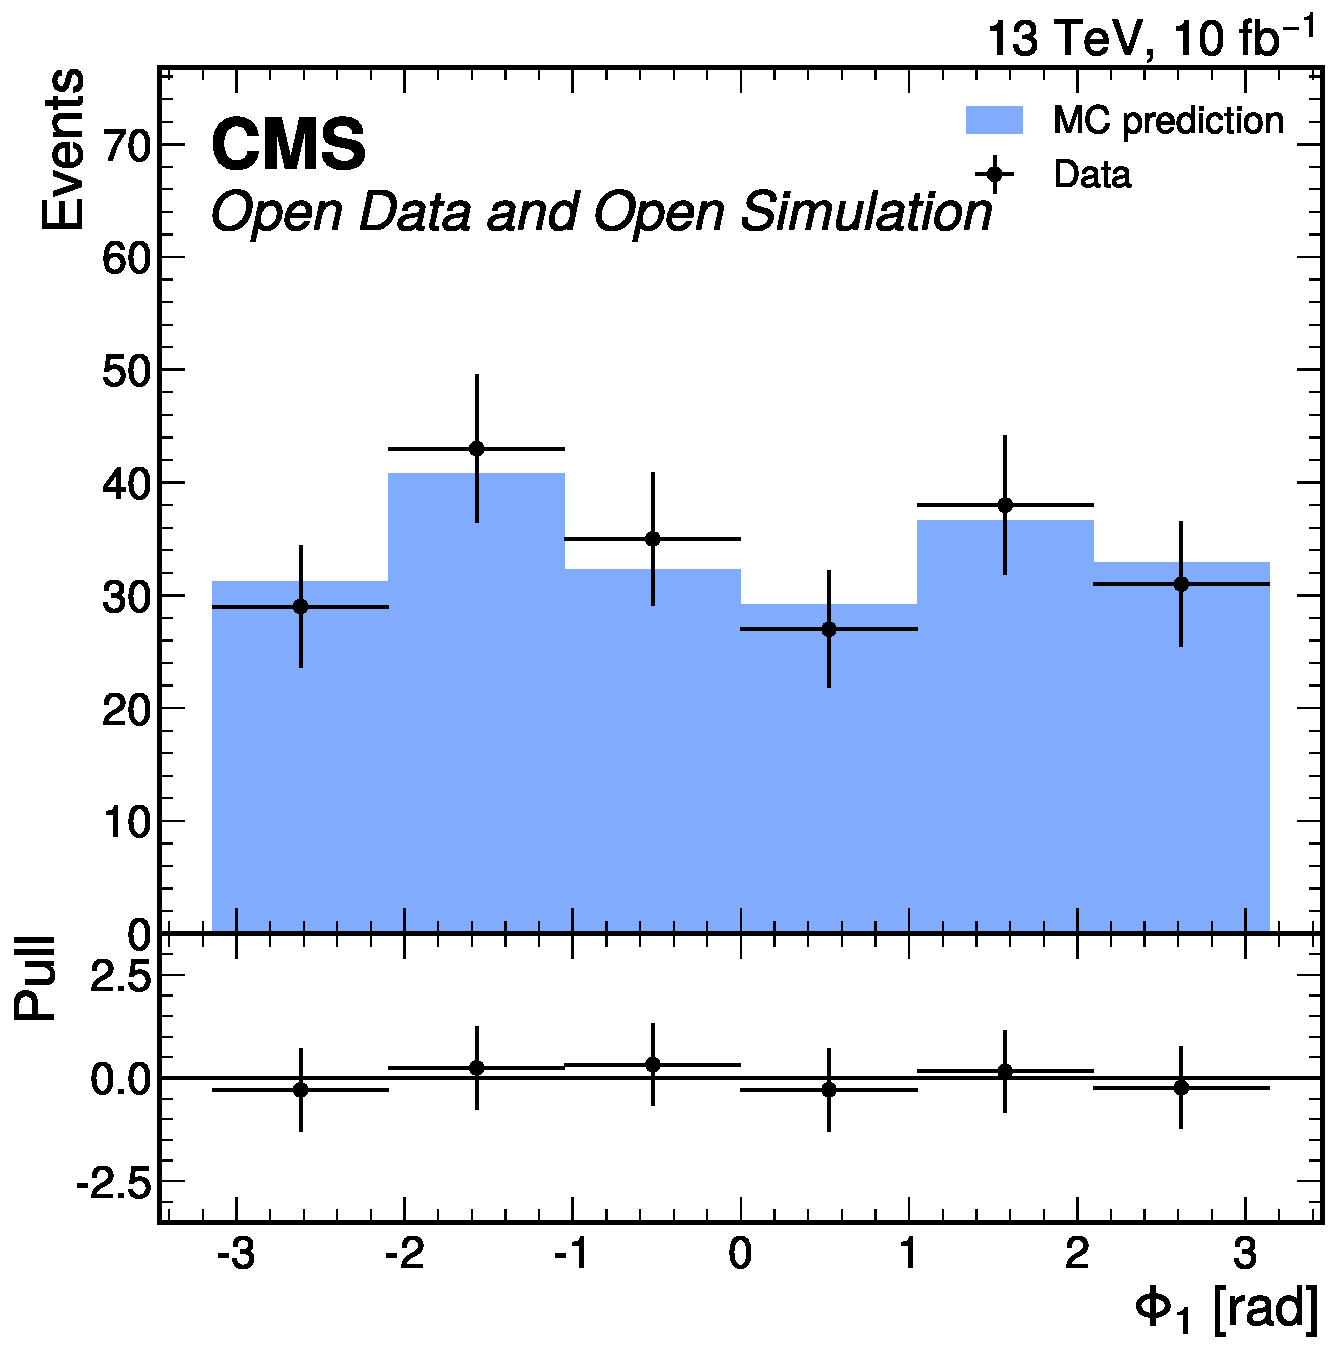
\includegraphics[width=0.92\linewidth,height=0.70\textheight,keepaspectratio]{figures/input_validation_phi1.pdf}
\caption{Phi\_1 [rad] input-validation distribution in the broad $70 \le m_{4\ell} \le 170$ GeV window. The D7 shape gate passes with chi2/ndf = 0.155 and p = 0.979; this comparison is used only to decide classifier-input eligibility, not to normalize fit templates.}
\label{fig:input-validation-phi1}
\end{figure}

\begin{figure}[p]
\centering
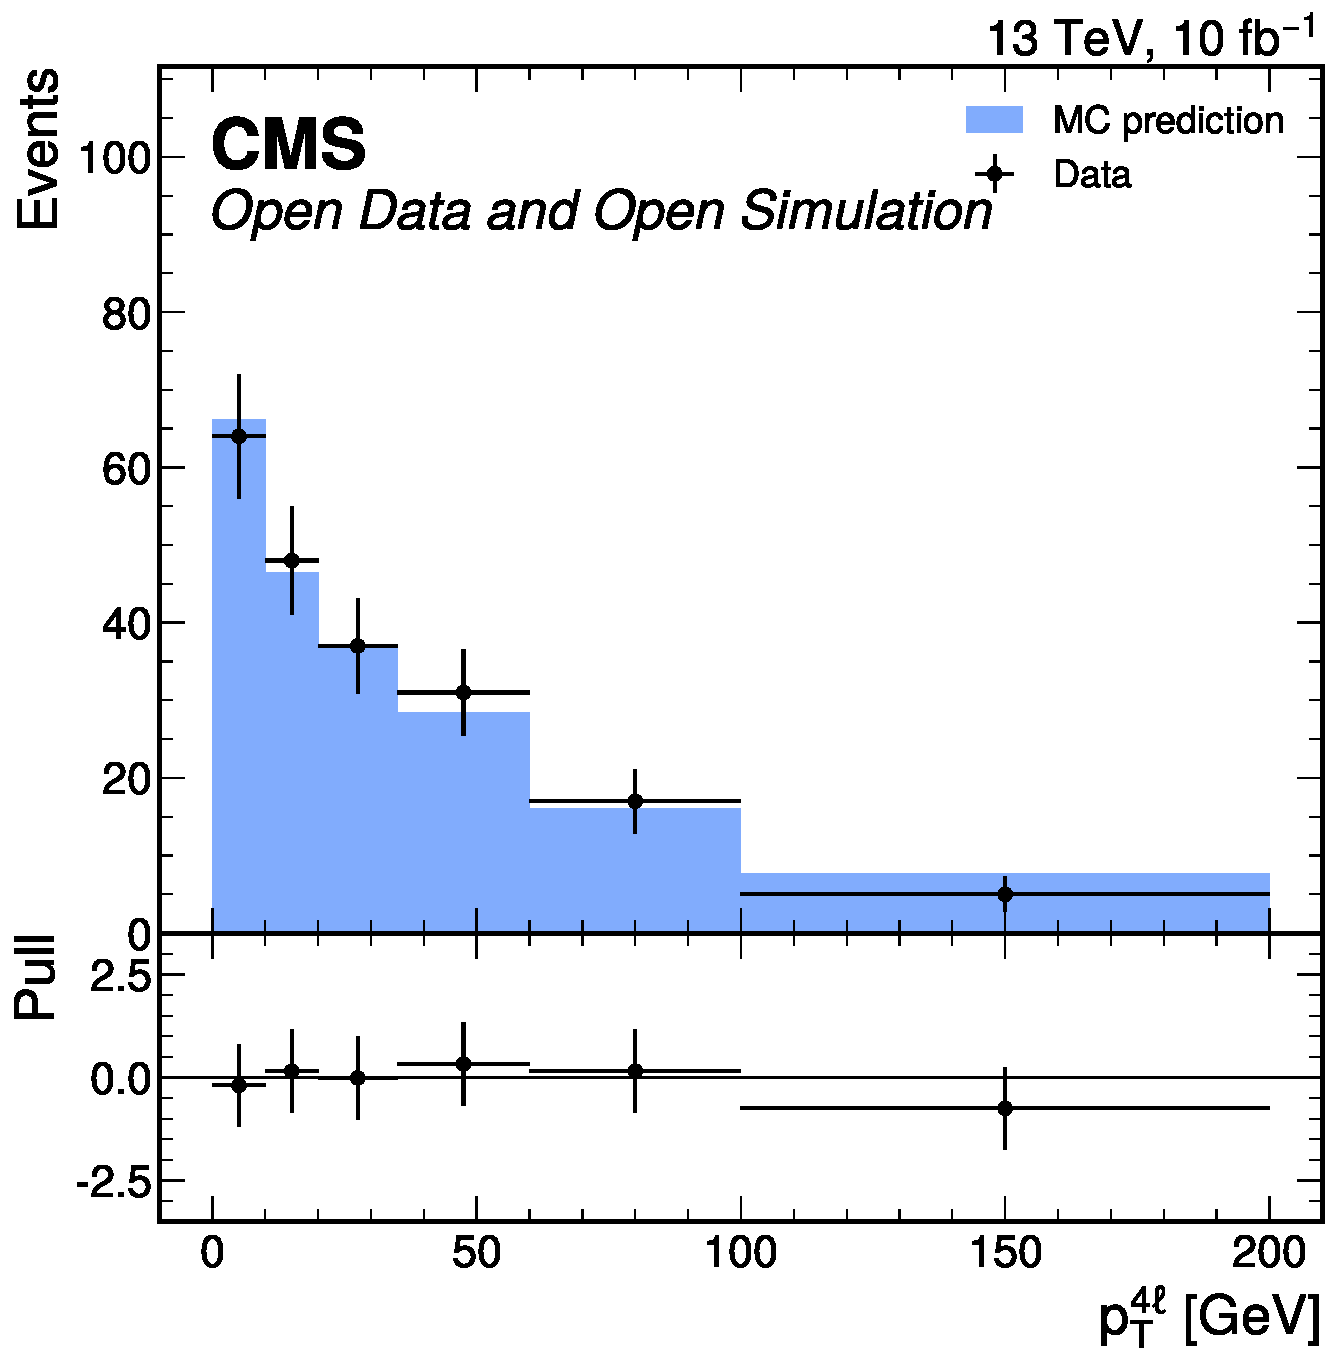
\includegraphics[width=0.92\linewidth,height=0.70\textheight,keepaspectratio]{figures/input_validation_pt4l.pdf}
\caption{p\_T\textasciicircum{}\{4ell\} [GeV] input-validation distribution in the broad $70 \le m_{4\ell} \le 170$ GeV window. The D7 shape gate fails with chi2/ndf = 0.333 and p = 0.893; this comparison is used only to decide classifier-input eligibility, not to normalize fit templates.}
\label{fig:input-validation-pt4l}
\end{figure}

\begin{figure}[p]
\centering
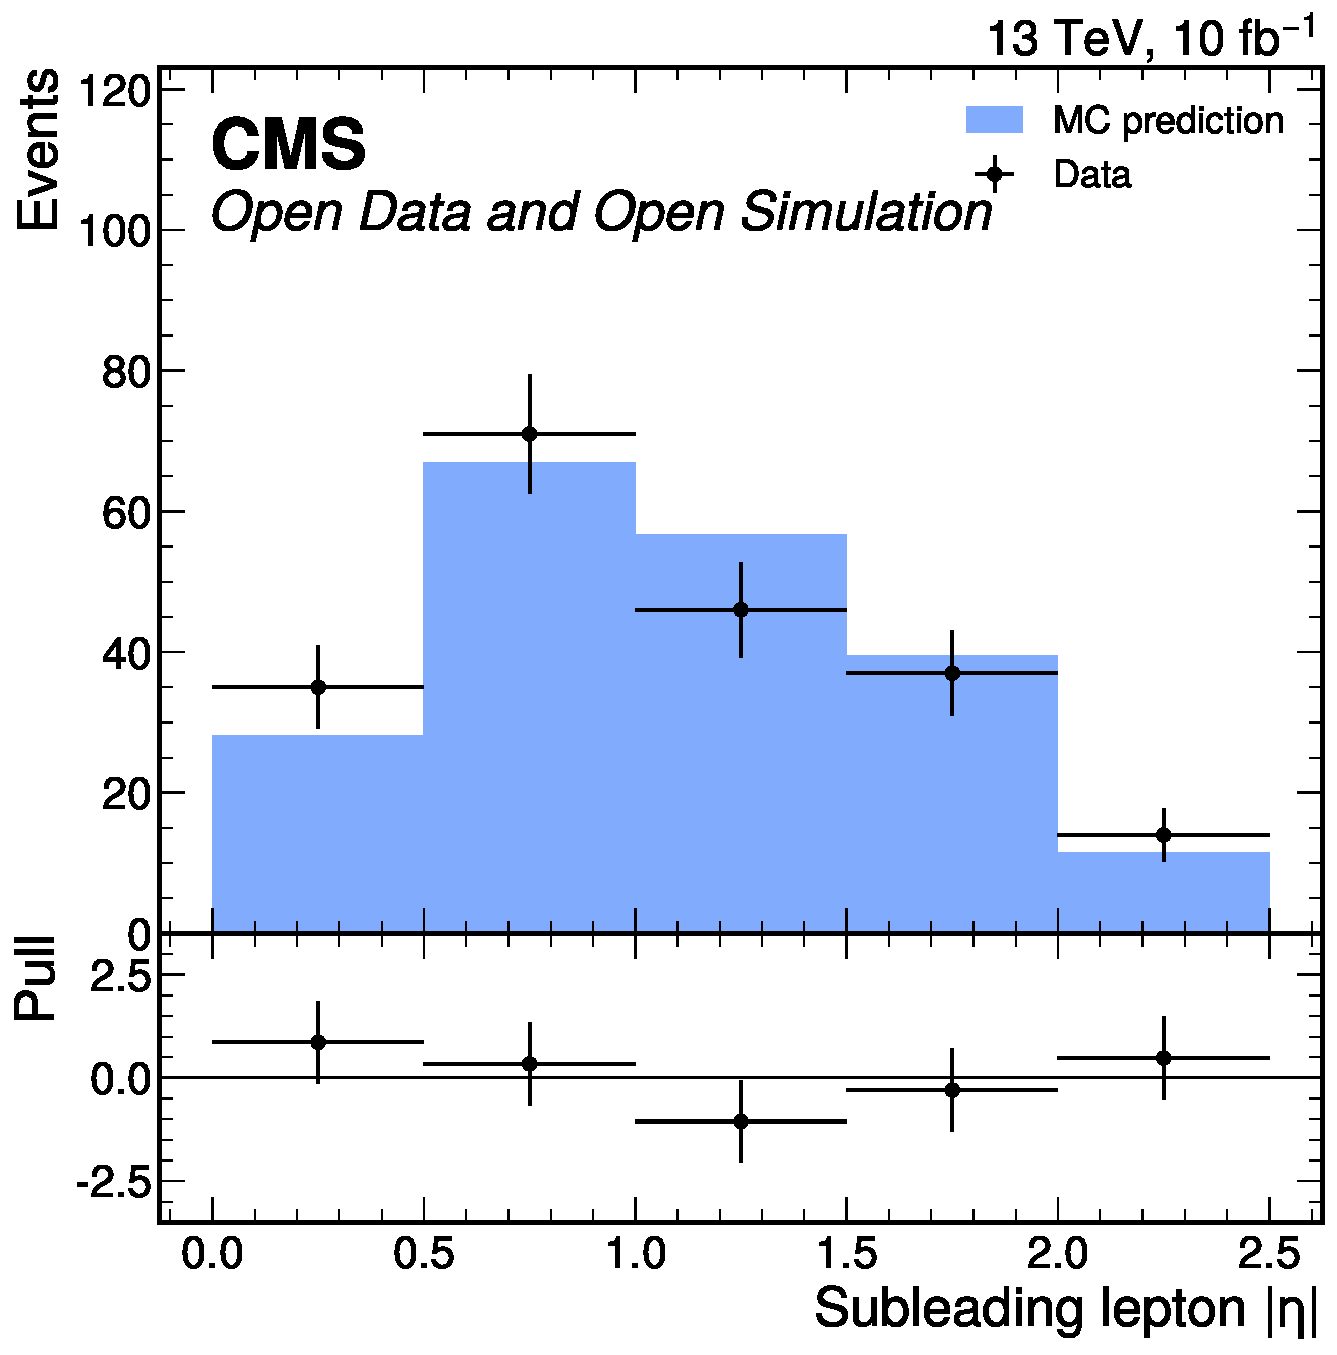
\includegraphics[width=0.92\linewidth,height=0.70\textheight,keepaspectratio]{figures/input_validation_sublead_abs_eta.pdf}
\caption{Subleading lepton |eta| input-validation distribution in the broad $70 \le m_{4\ell} \le 170$ GeV window. The D7 shape gate fails with chi2/ndf = 1.08 and p = 0.366; this comparison is used only to decide classifier-input eligibility, not to normalize fit templates.}
\label{fig:input-validation-sublead-abs-eta}
\end{figure}

\begin{figure}[p]
\centering
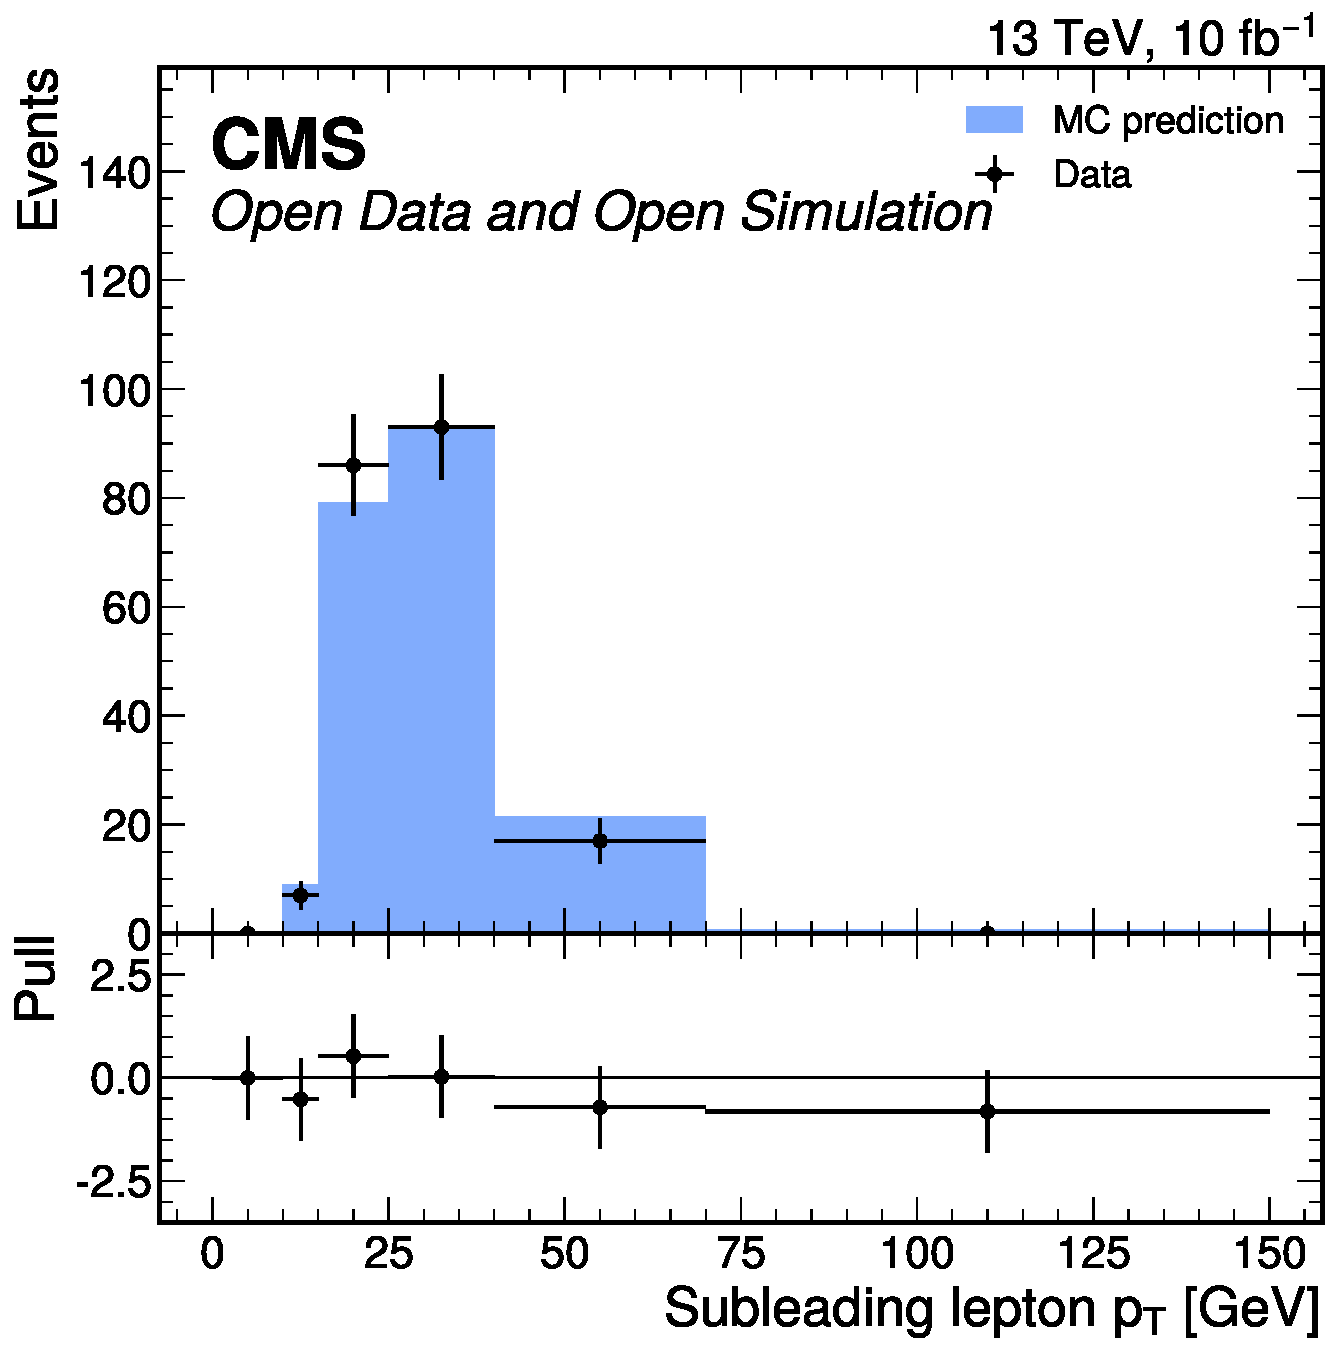
\includegraphics[width=0.92\linewidth,height=0.70\textheight,keepaspectratio]{figures/input_validation_sublead_lepton_pt.pdf}
\caption{Subleading lepton p\_T [GeV] input-validation distribution in the broad $70 \le m_{4\ell} \le 170$ GeV window. The D7 shape gate fails with chi2/ndf = 849.48 and p = 0.0; this comparison is used only to decide classifier-input eligibility, not to normalize fit templates.}
\label{fig:input-validation-sublead-lepton-pt}
\end{figure}

\begin{figure}[p]
\centering
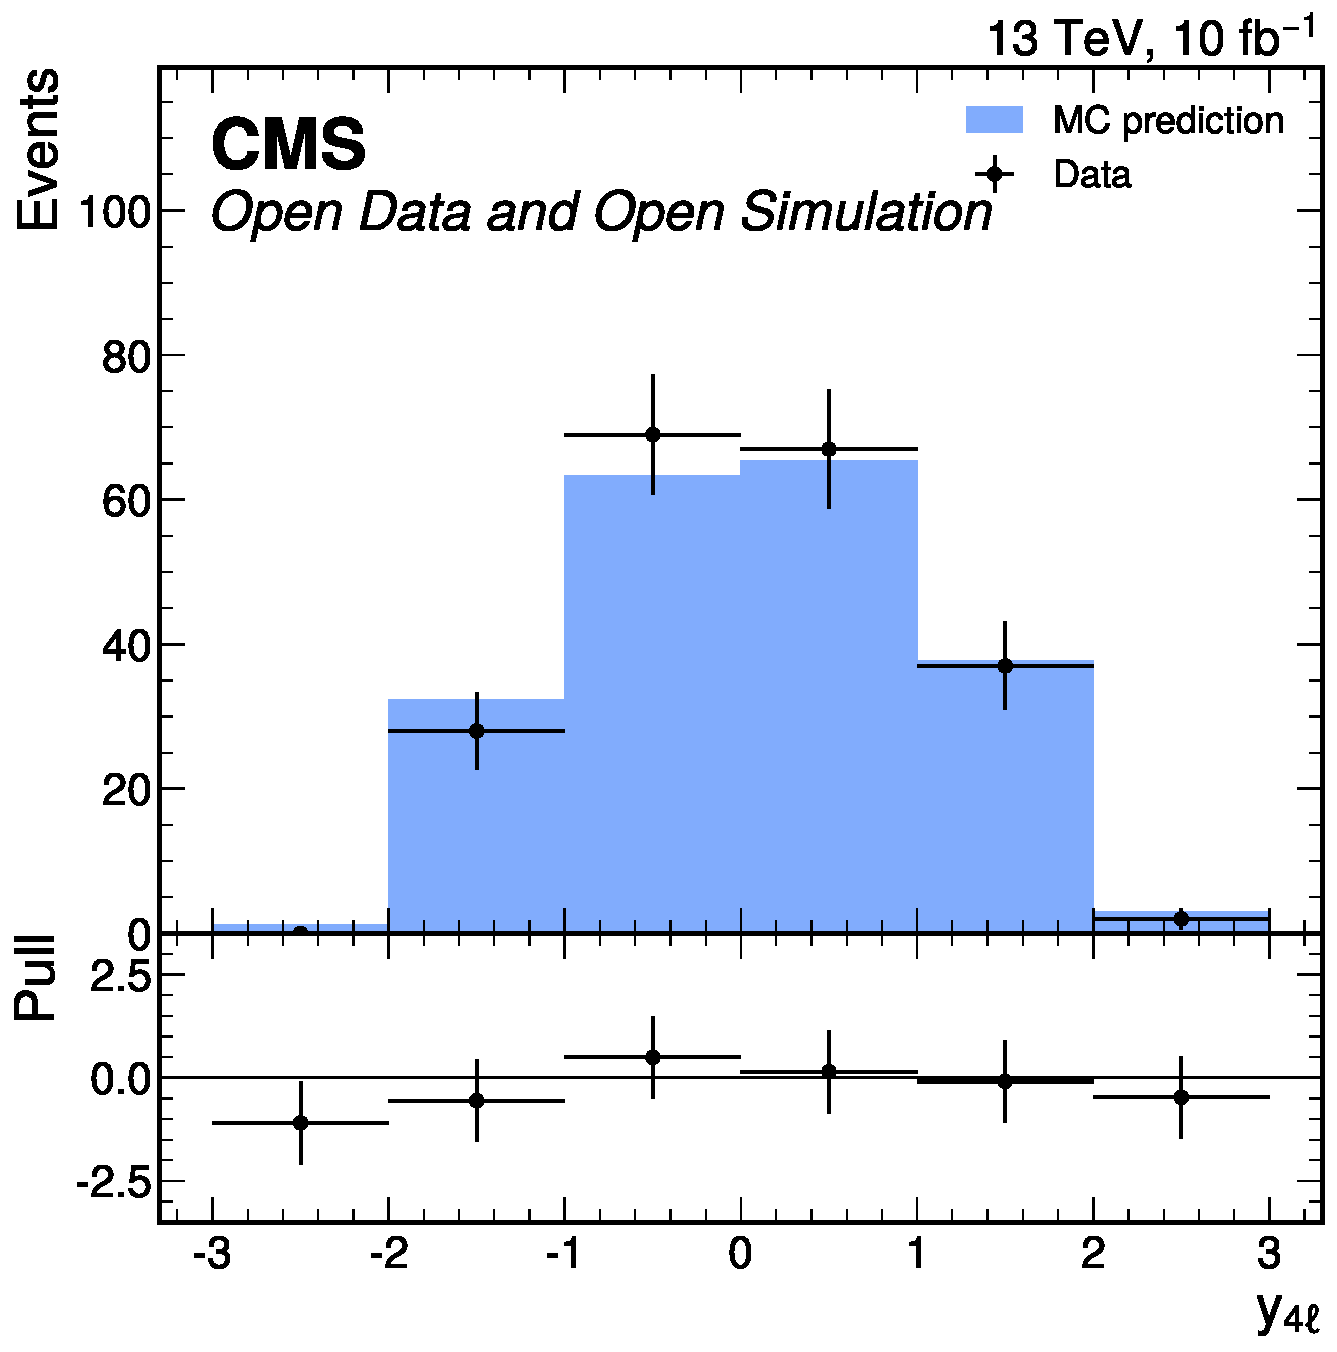
\includegraphics[width=0.92\linewidth,height=0.70\textheight,keepaspectratio]{figures/input_validation_y4l.pdf}
\caption{y\_\{4ell\} input-validation distribution in the broad $70 \le m_{4\ell} \le 170$ GeV window. The D7 shape gate fails with chi2/ndf = 996.68 and p = 0.0; this comparison is used only to decide classifier-input eligibility, not to normalize fit templates.}
\label{fig:input-validation-y4l}
\end{figure}

\begin{figure}[p]
\centering
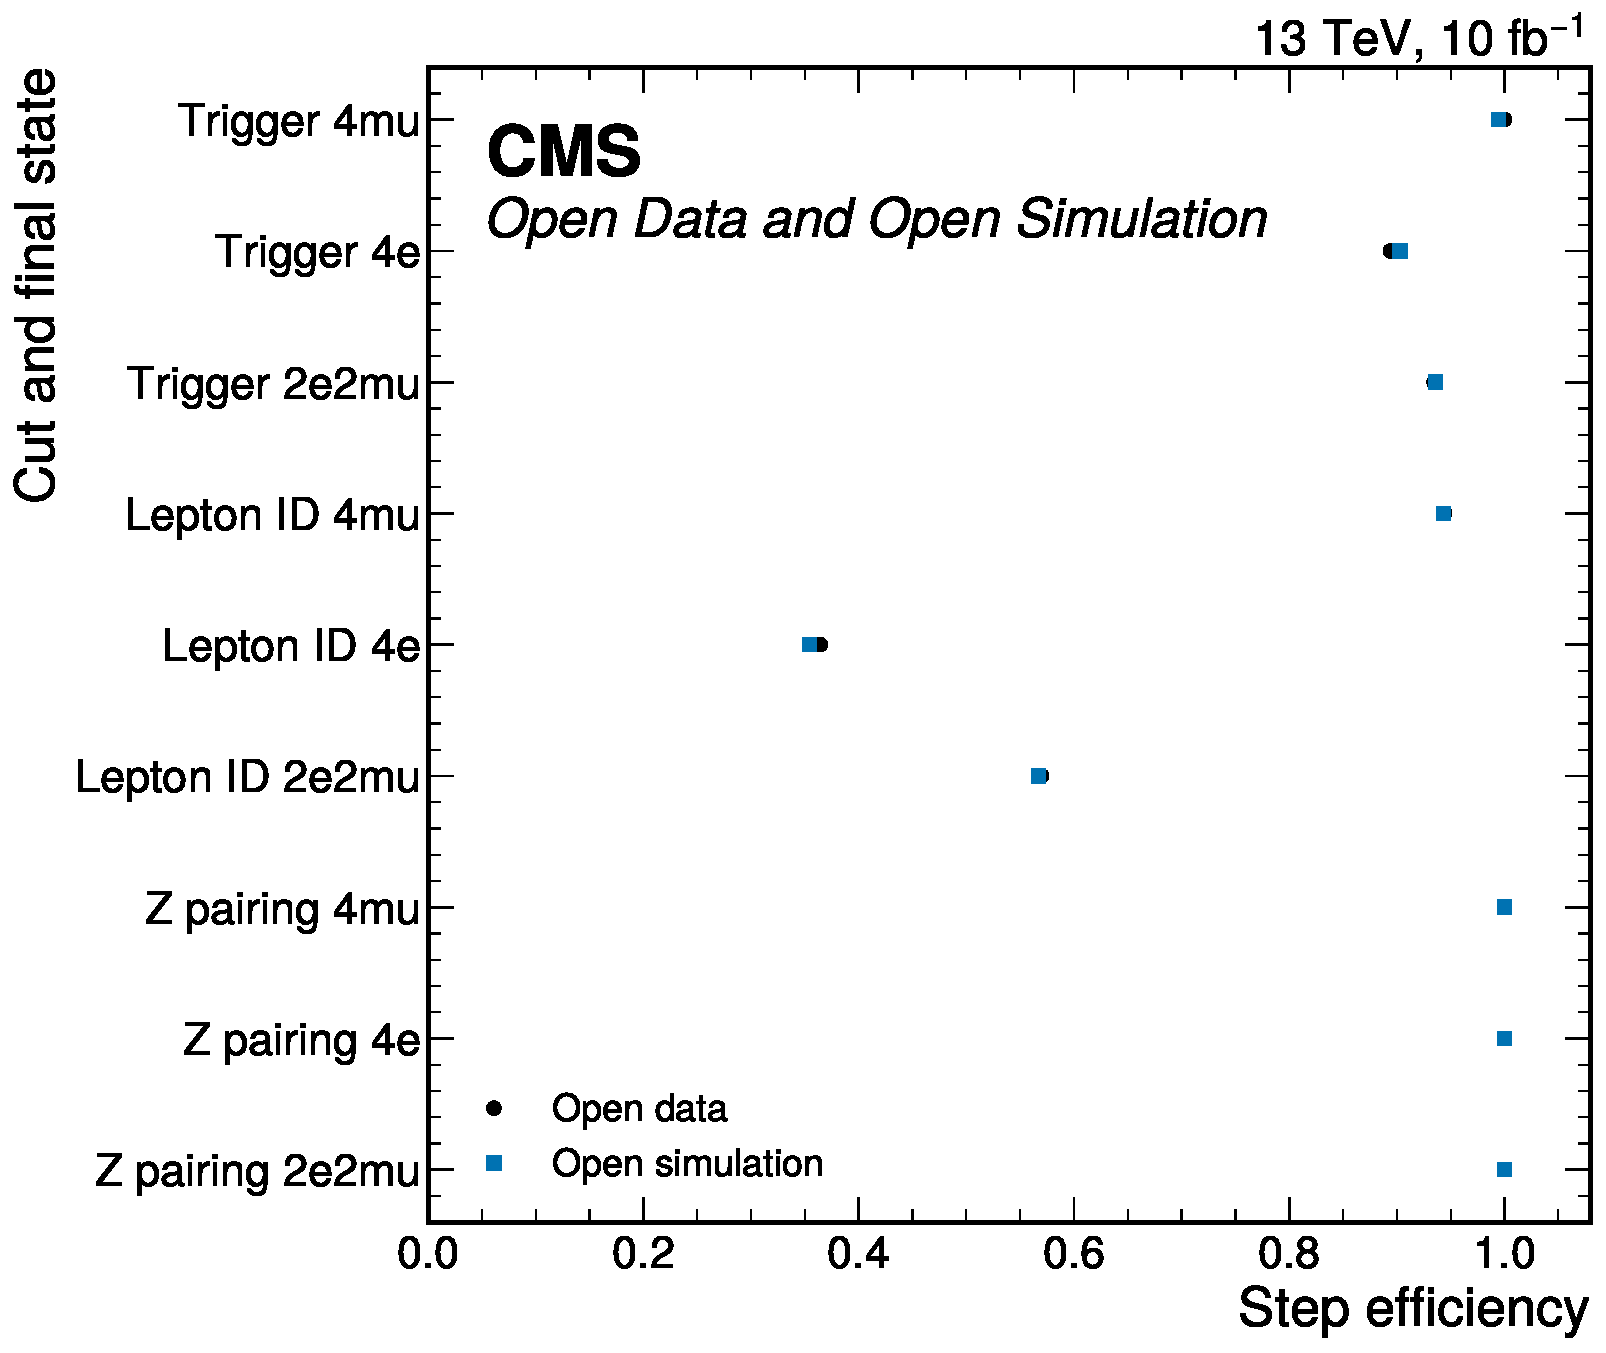
\includegraphics[width=0.92\linewidth,height=0.70\textheight,keepaspectratio]{figures/cut_motivation_efficiencies.pdf}
\caption{Trigger, flavor-matched lepton-ID, and Z-pair sanity efficiencies by final state. Efficiencies are ratios to the previous predeclared selection step; data uses raw events and MC uses prompt-normalized weighted yields.}
\label{fig:cut-motivation-efficiencies}
\end{figure}

\begin{figure}[p]
\centering
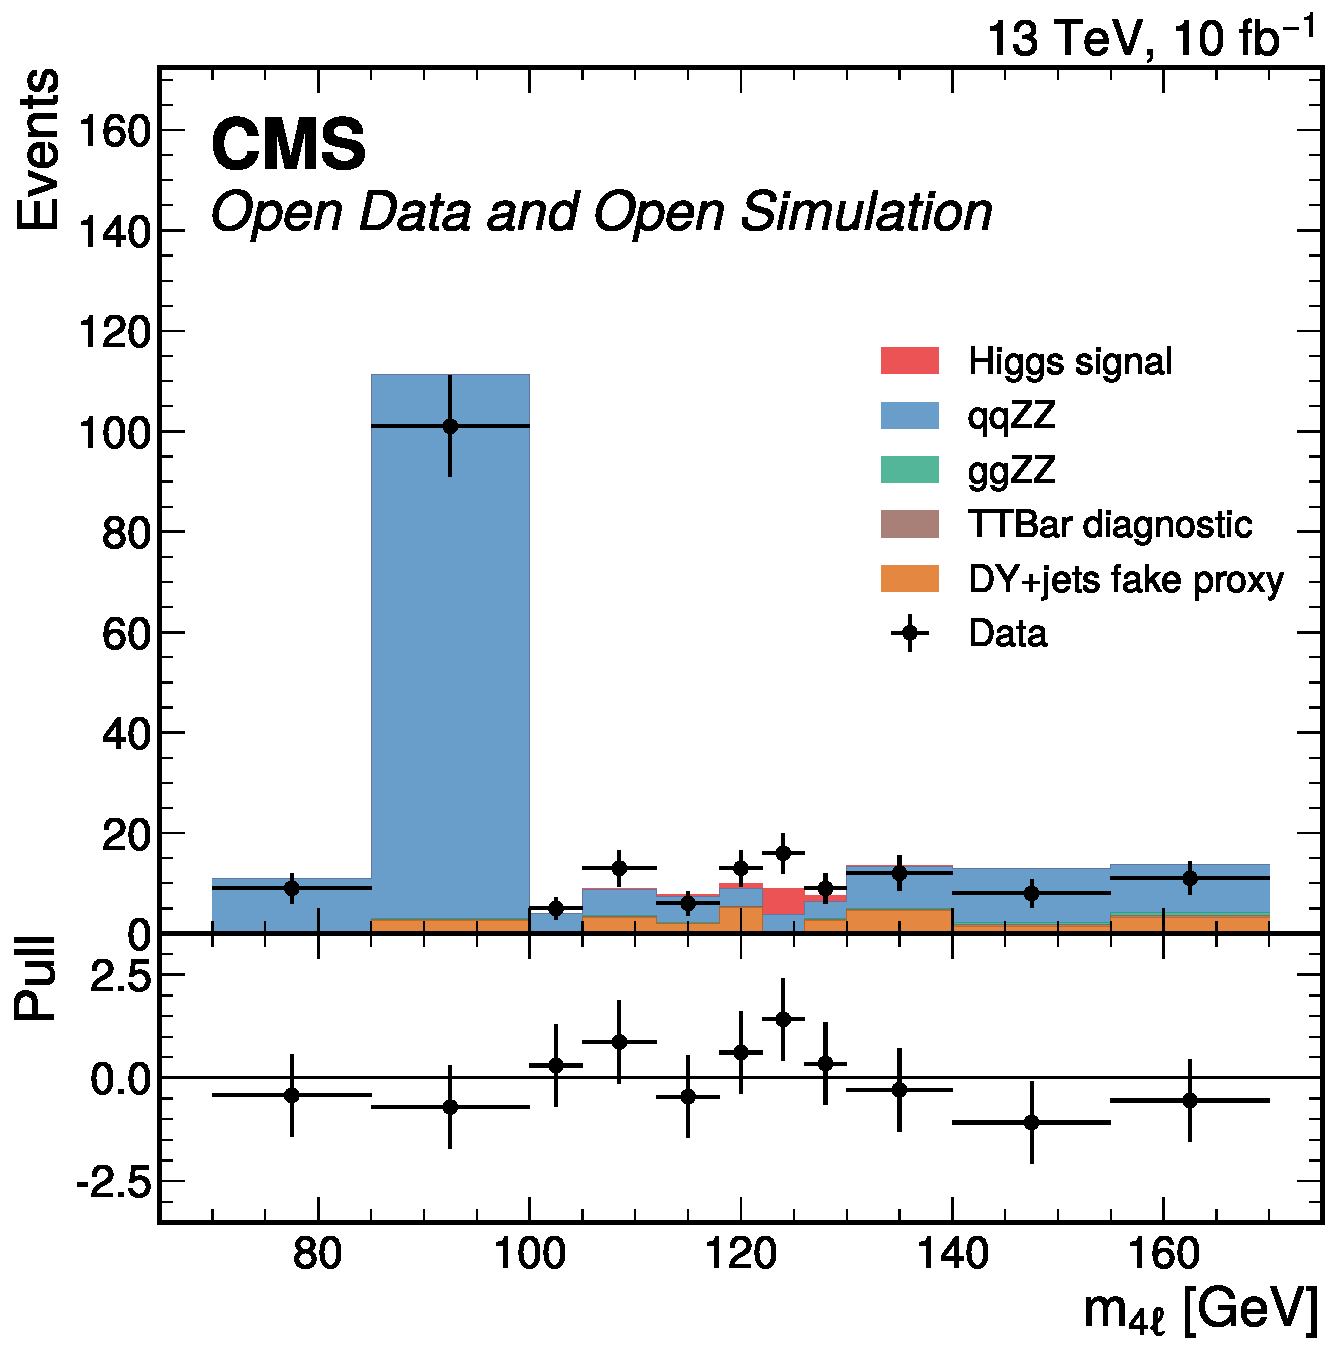
\includegraphics[width=0.92\linewidth,height=0.70\textheight,keepaspectratio]{figures/m4l_broad_window_inclusive.pdf}
\caption{Inclusive four-lepton mass distribution in the broad validation window. MC is normalized with prompt effective cross sections and Metadata denominators, while DY+jets remains the nominal fake proxy. This display is sideband and validation context for the broad-window result; the Phase 4c observed result fits the 70--170 GeV window directly.}
\label{fig:m4l-broad-window-inclusive}
\end{figure}

\begin{figure}[p]
\centering
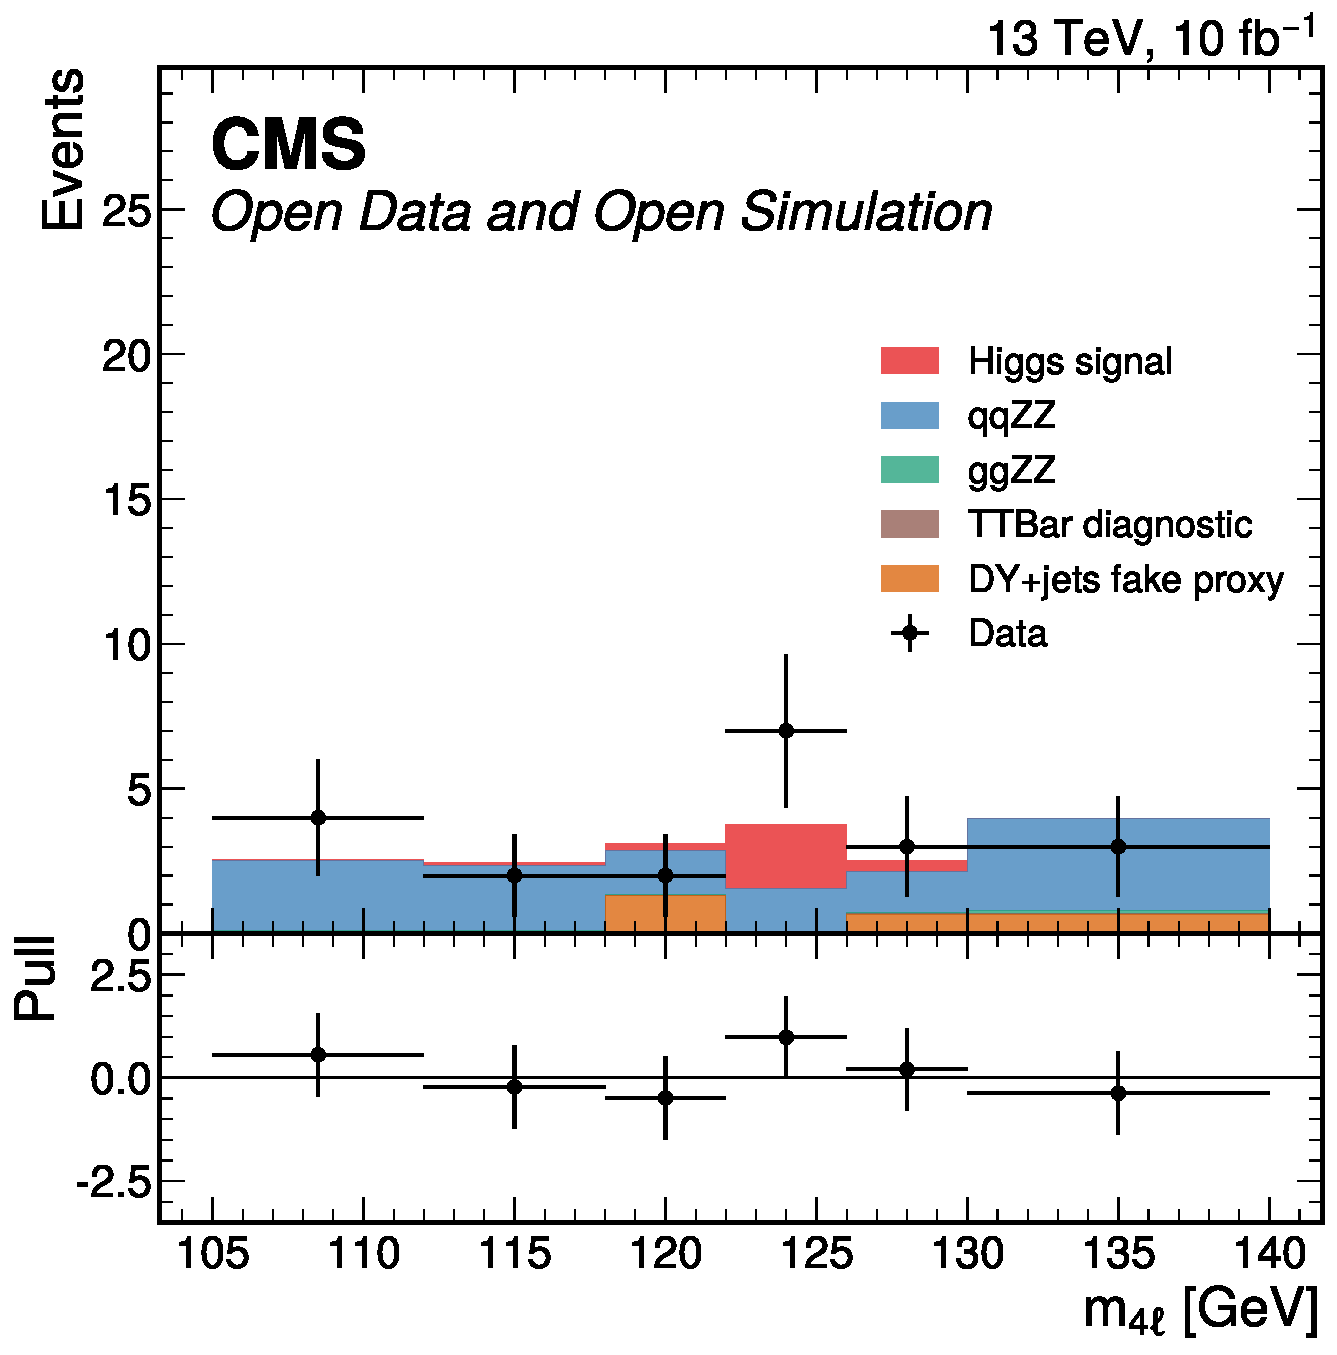
\includegraphics[width=0.92\linewidth,height=0.70\textheight,keepaspectratio]{figures/m4l_fit_4mu.pdf}
\caption{Historical narrow-window 4mu category diagnostic retained from Phase 3. The current signal-strength result uses the broad 70--170 GeV observed final-state templates; no real VBF category is available and classifier categories remain unpromoted.}
\label{fig:m4l-fit-4mu}
\end{figure}

\begin{figure}[p]
\centering
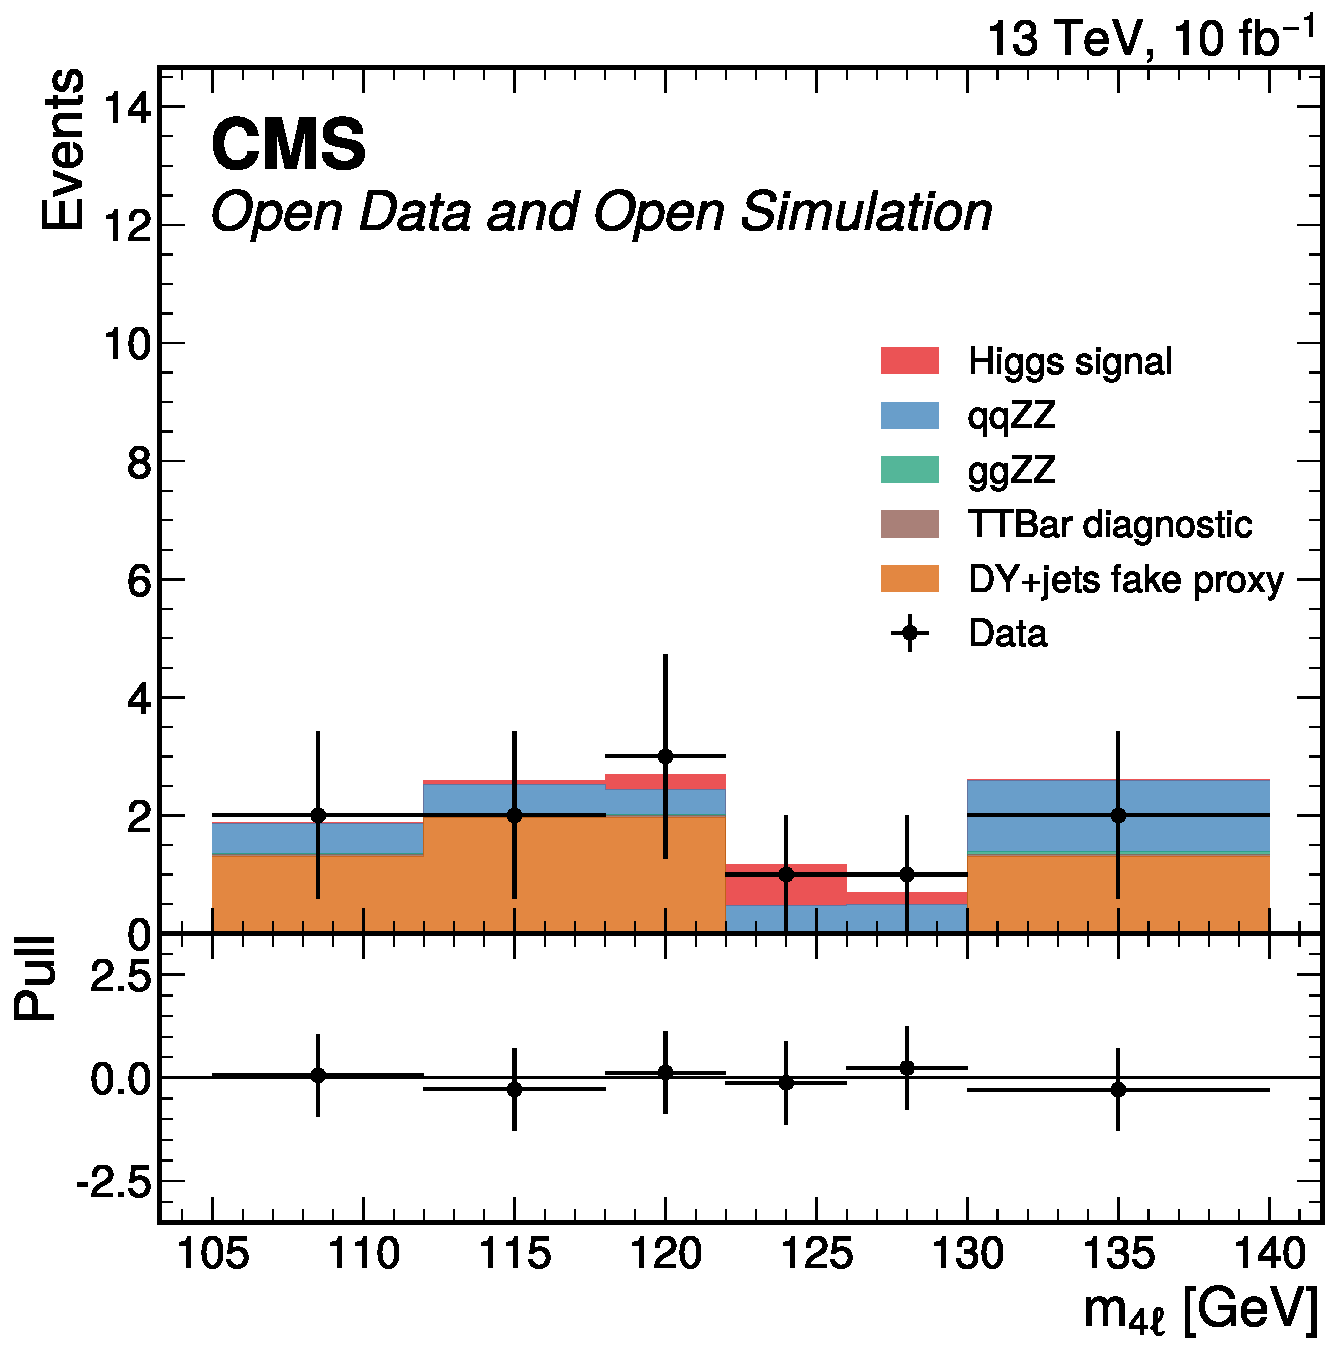
\includegraphics[width=0.92\linewidth,height=0.70\textheight,keepaspectratio]{figures/m4l_fit_4e.pdf}
\caption{Historical narrow-window 4e category diagnostic retained from Phase 3. The current signal-strength result uses the broad 70--170 GeV observed final-state templates; no real VBF category is available and classifier categories remain unpromoted.}
\label{fig:m4l-fit-4e}
\end{figure}

\begin{figure}[p]
\centering
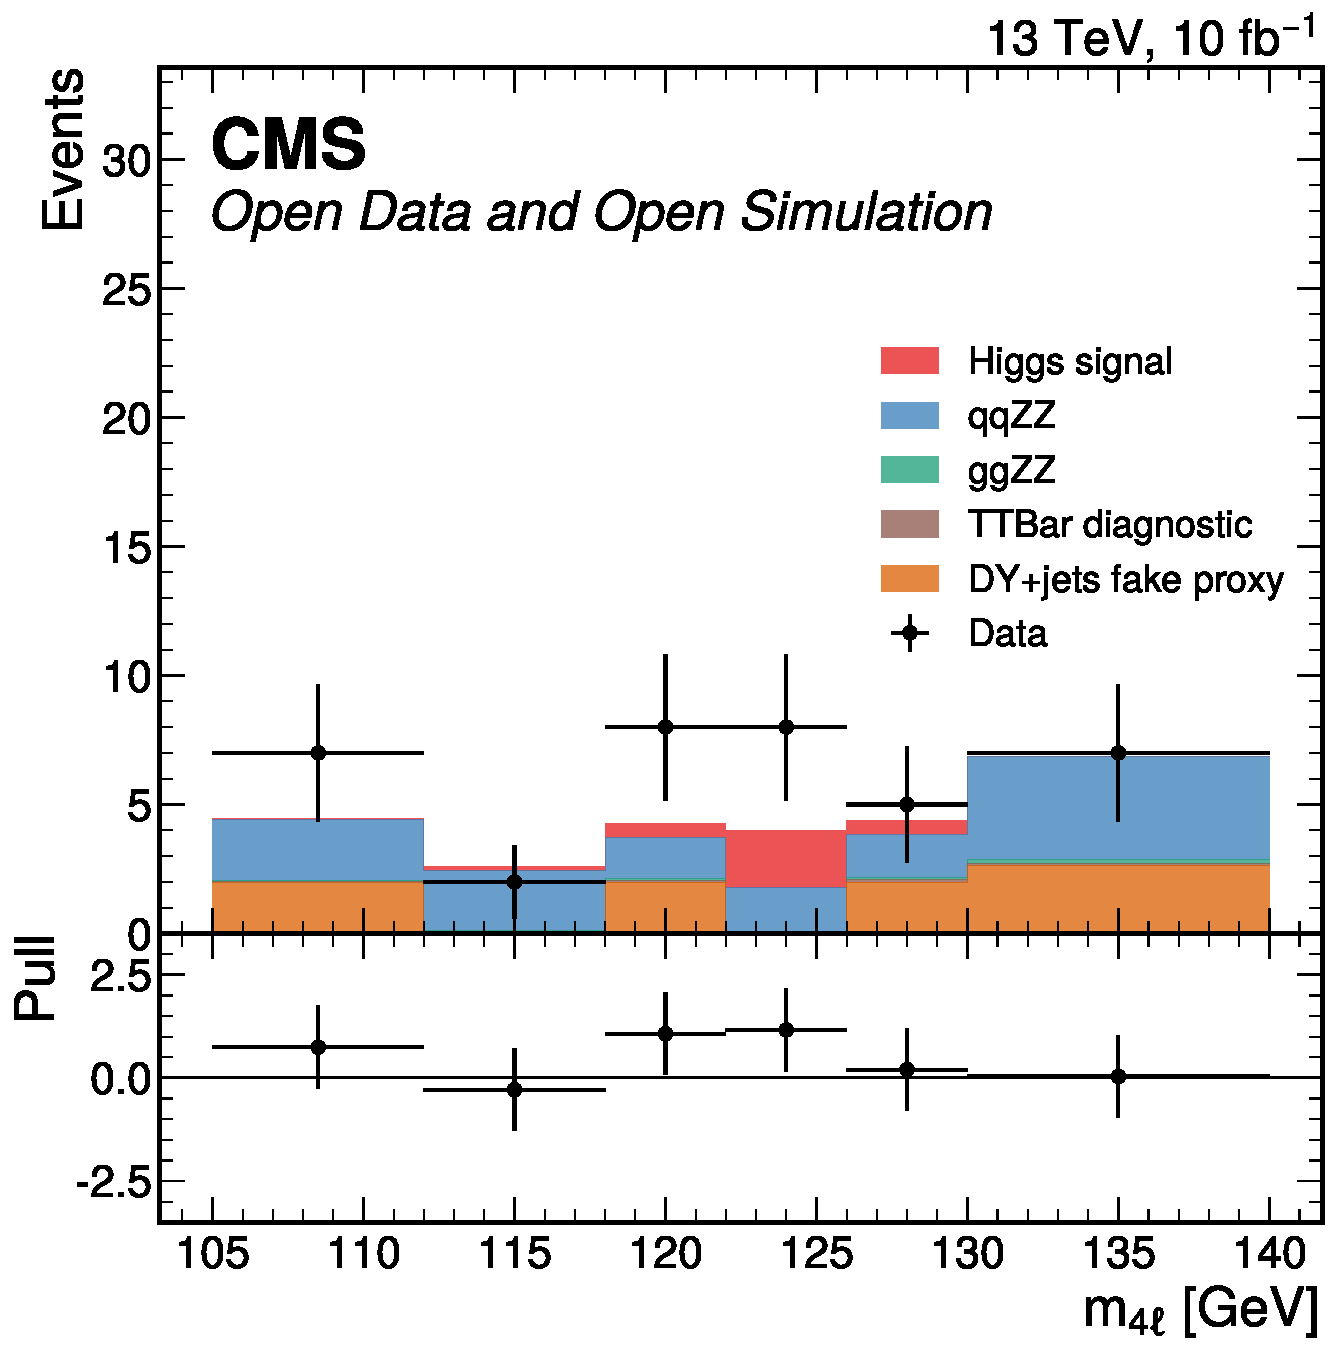
\includegraphics[width=0.92\linewidth,height=0.70\textheight,keepaspectratio]{figures/m4l_fit_2e2mu.pdf}
\caption{Historical narrow-window 2e2mu category diagnostic retained from Phase 3. The current signal-strength result uses the broad 70--170 GeV observed final-state templates; no real VBF category is available and classifier categories remain unpromoted.}
\label{fig:m4l-fit-2e2mu}
\end{figure}

\begin{figure}[p]
\centering
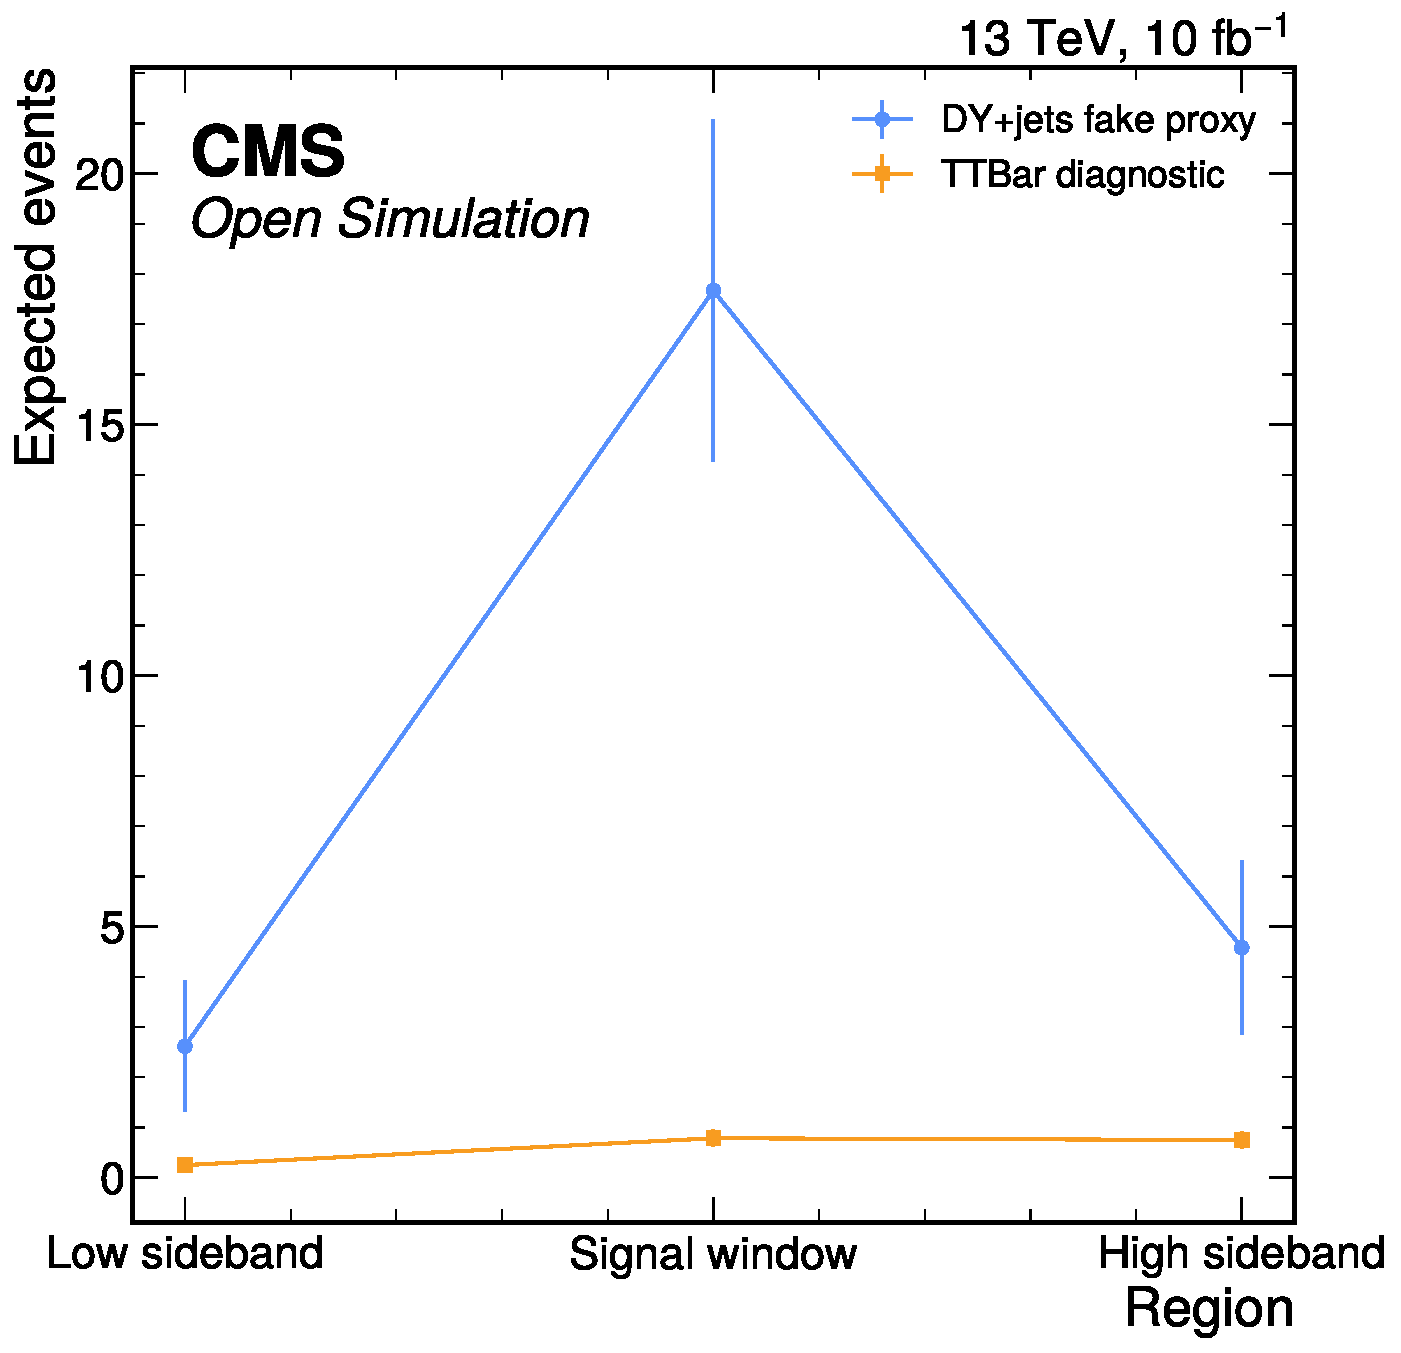
\includegraphics[width=0.92\linewidth,height=0.70\textheight,keepaspectratio]{figures/sideband_dy_ttbar_diagnostics.pdf}
\caption{DY+jets fake proxy and TTBar diagnostic reducible-background checks across the predeclared sideband and signal regions. The TTBar diagnostic to DY+jets fake-proxy ratios are 0.16 in the high sideband, 0.10 in the low sideband, and 0.044 in the signal window, so TTBar is not promoted to the nominal fake model by the Phase 2 thresholds.}
\label{fig:sideband-dy-ttbar-diagnostics}
\end{figure}

\begin{figure}[p]
\centering
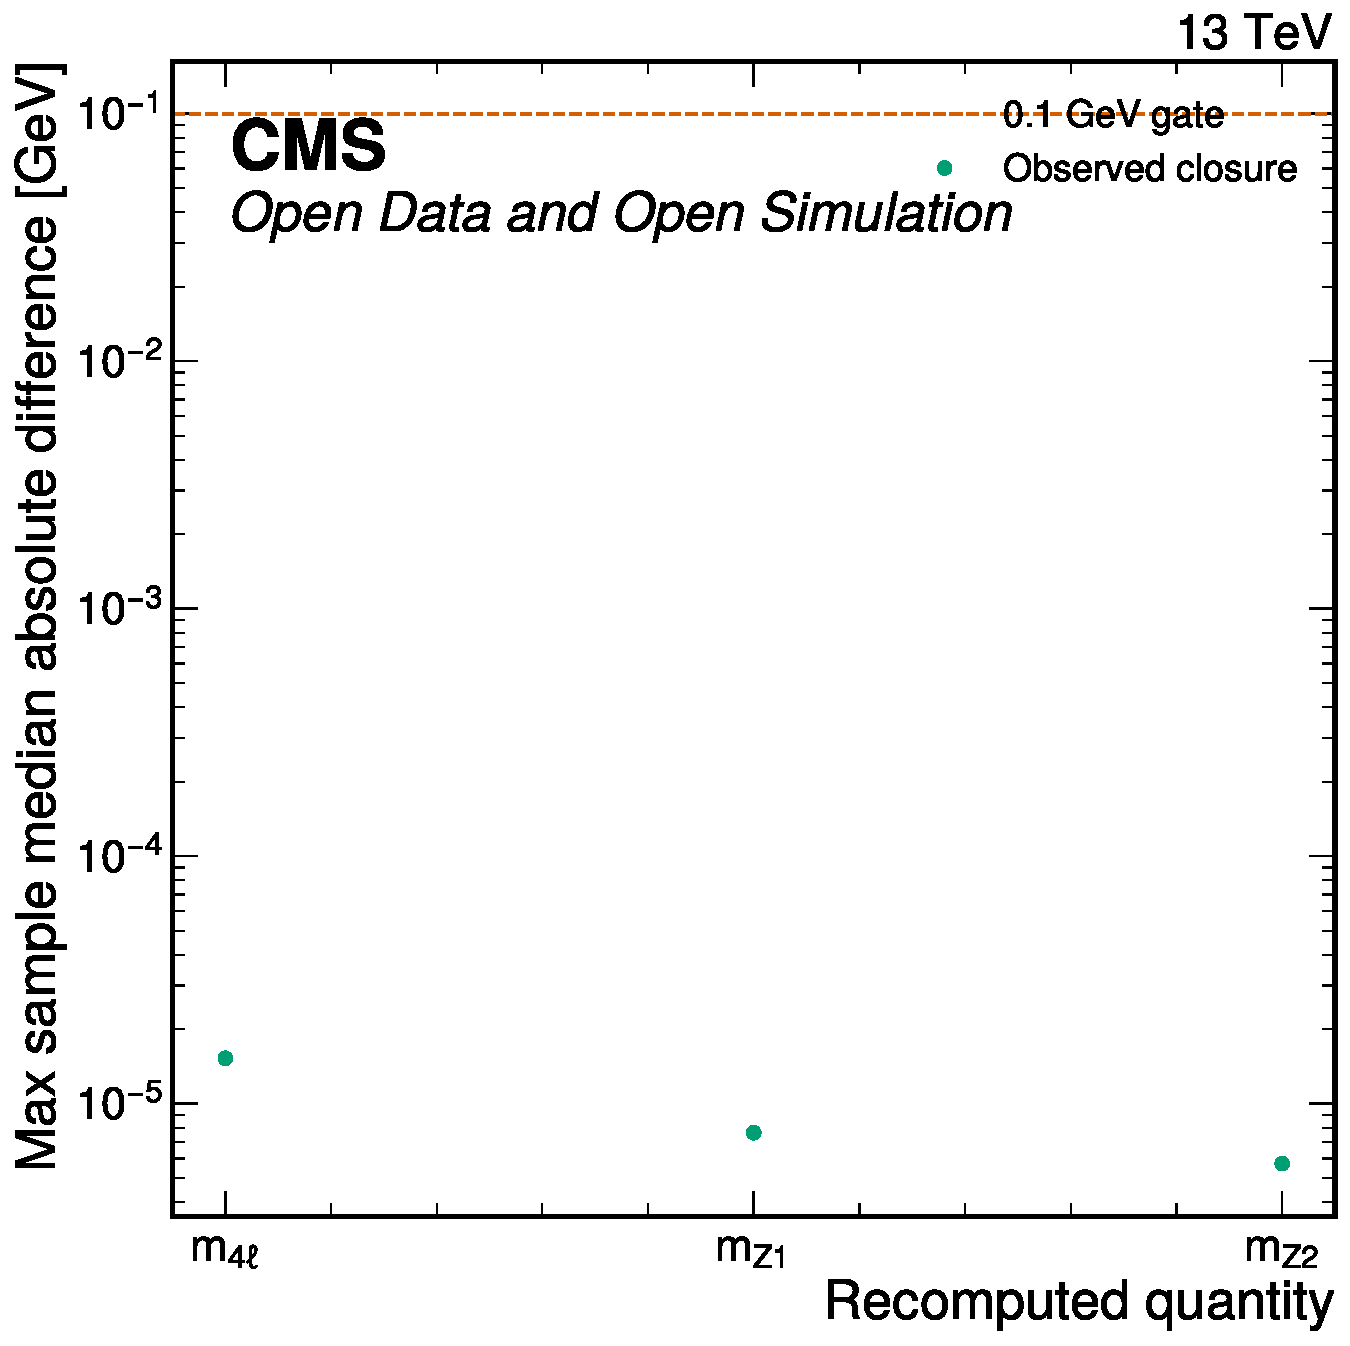
\includegraphics[width=0.92\linewidth,height=0.70\textheight,keepaspectratio]{figures/angular_closure_median_deltas.pdf}
\caption{Angular reco closure summary showing the maximum per-sample median absolute mass difference for recomputed four-vector quantities. All medians are far below the 0.1 GeV closure gate and all angular physical-range checks have zero out-of-range entries.}
\label{fig:angular-closure-median-deltas}
\end{figure}

\begin{figure}[p]
\centering
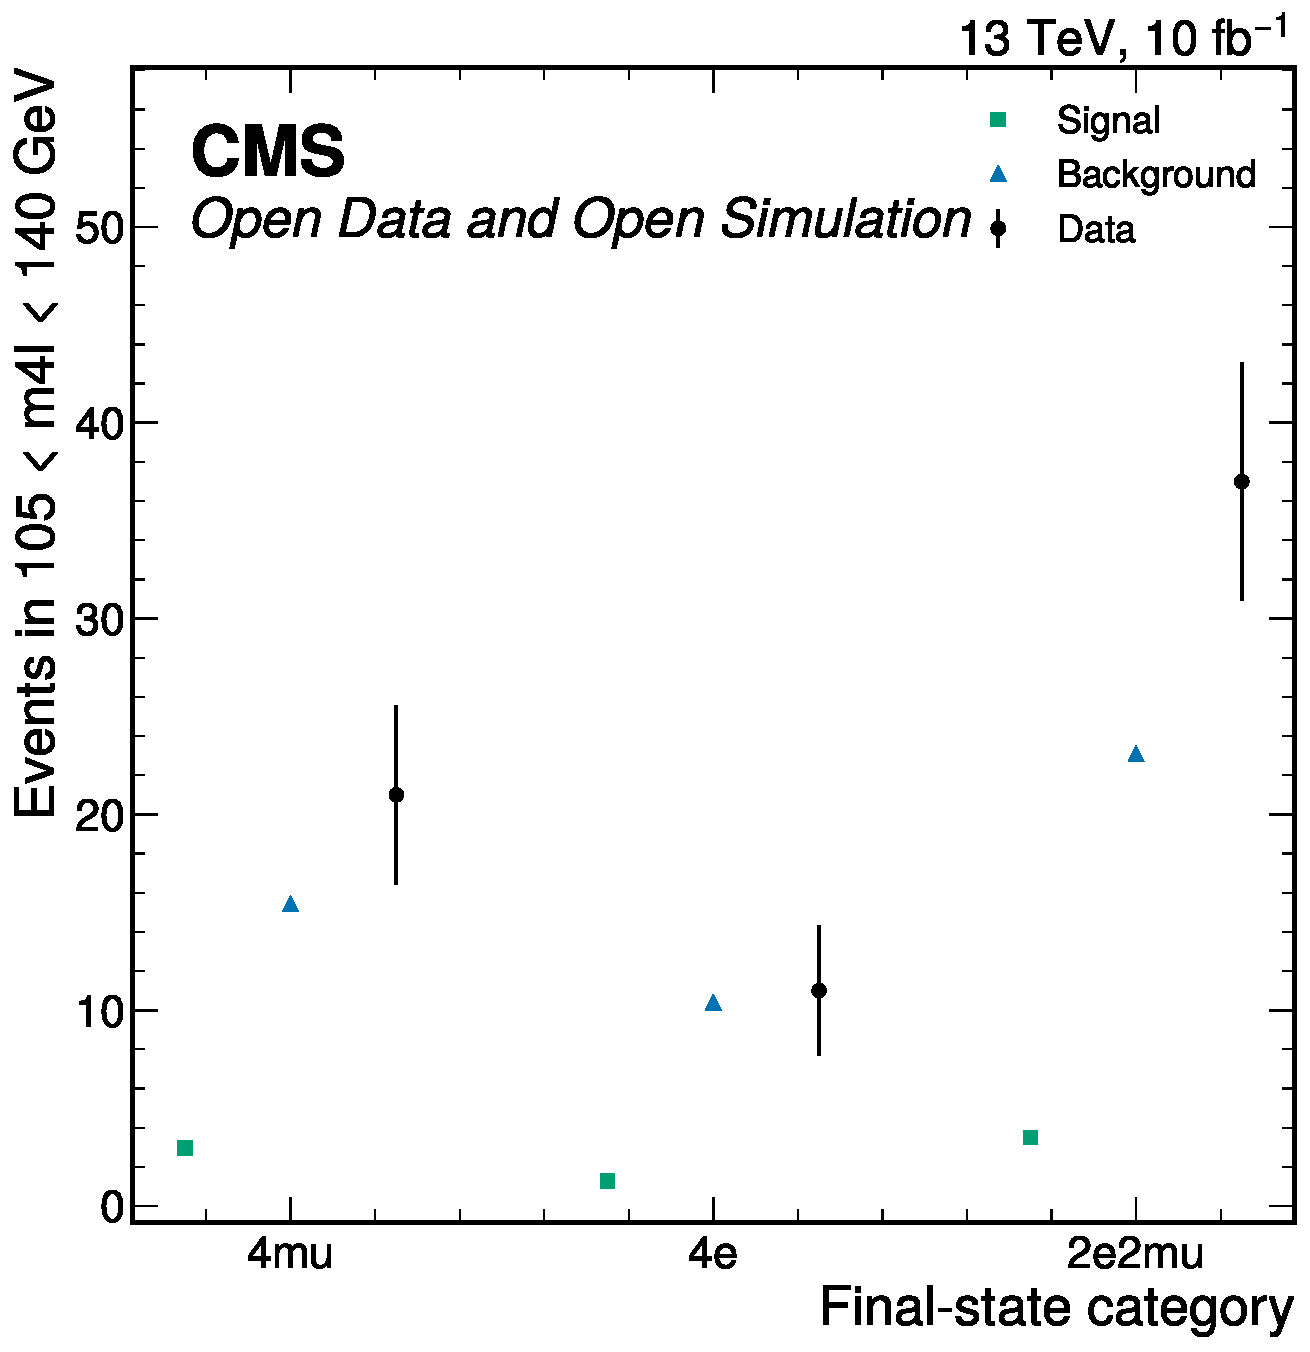
\includegraphics[width=0.92\linewidth,height=0.70\textheight,keepaspectratio]{figures/category_viability_s1.pdf}
\caption{S1 final-state category viability summary for the fit window. The categories are retained only as a conditional Phase 4 handoff: 17/18 final-state bins have S+B below five expected events, while S2 classifier categories fail low-stat viability.}
\label{fig:category-viability-s1}
\end{figure}

\begin{figure}[p]
\centering
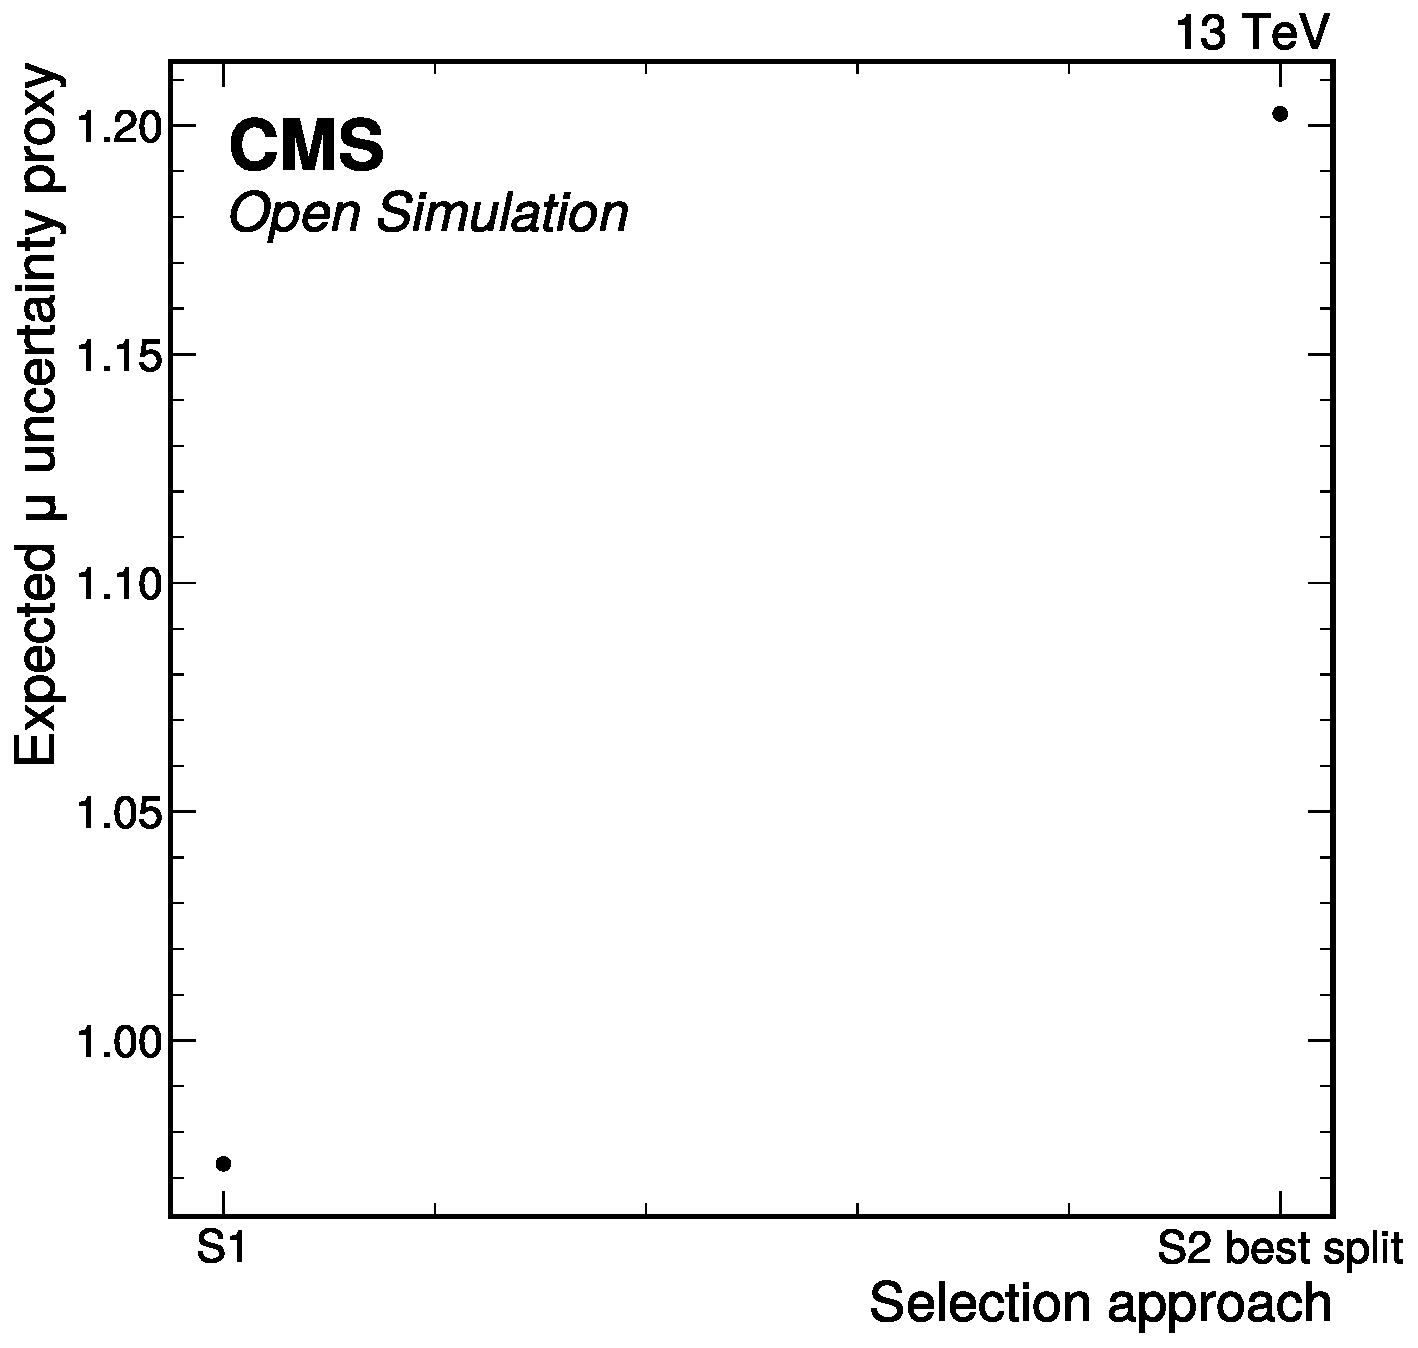
\includegraphics[width=0.92\linewidth,height=0.70\textheight,keepaspectratio]{figures/approach_comparison_mu_proxy.pdf}
\caption{S1 and S2 approach comparison using the common Asimov counting precision proxy. The nominal choice is S1\_reference\_like\_final\_state\_categories because S2 did not pass all input, score-shape, low-stat, overtraining, or >10\% improvement gates; final-state binning is a conditional low-count Phase 4 handoff.}
\label{fig:approach-comparison-mu-proxy}
\end{figure}

\begin{figure}[p]
\centering
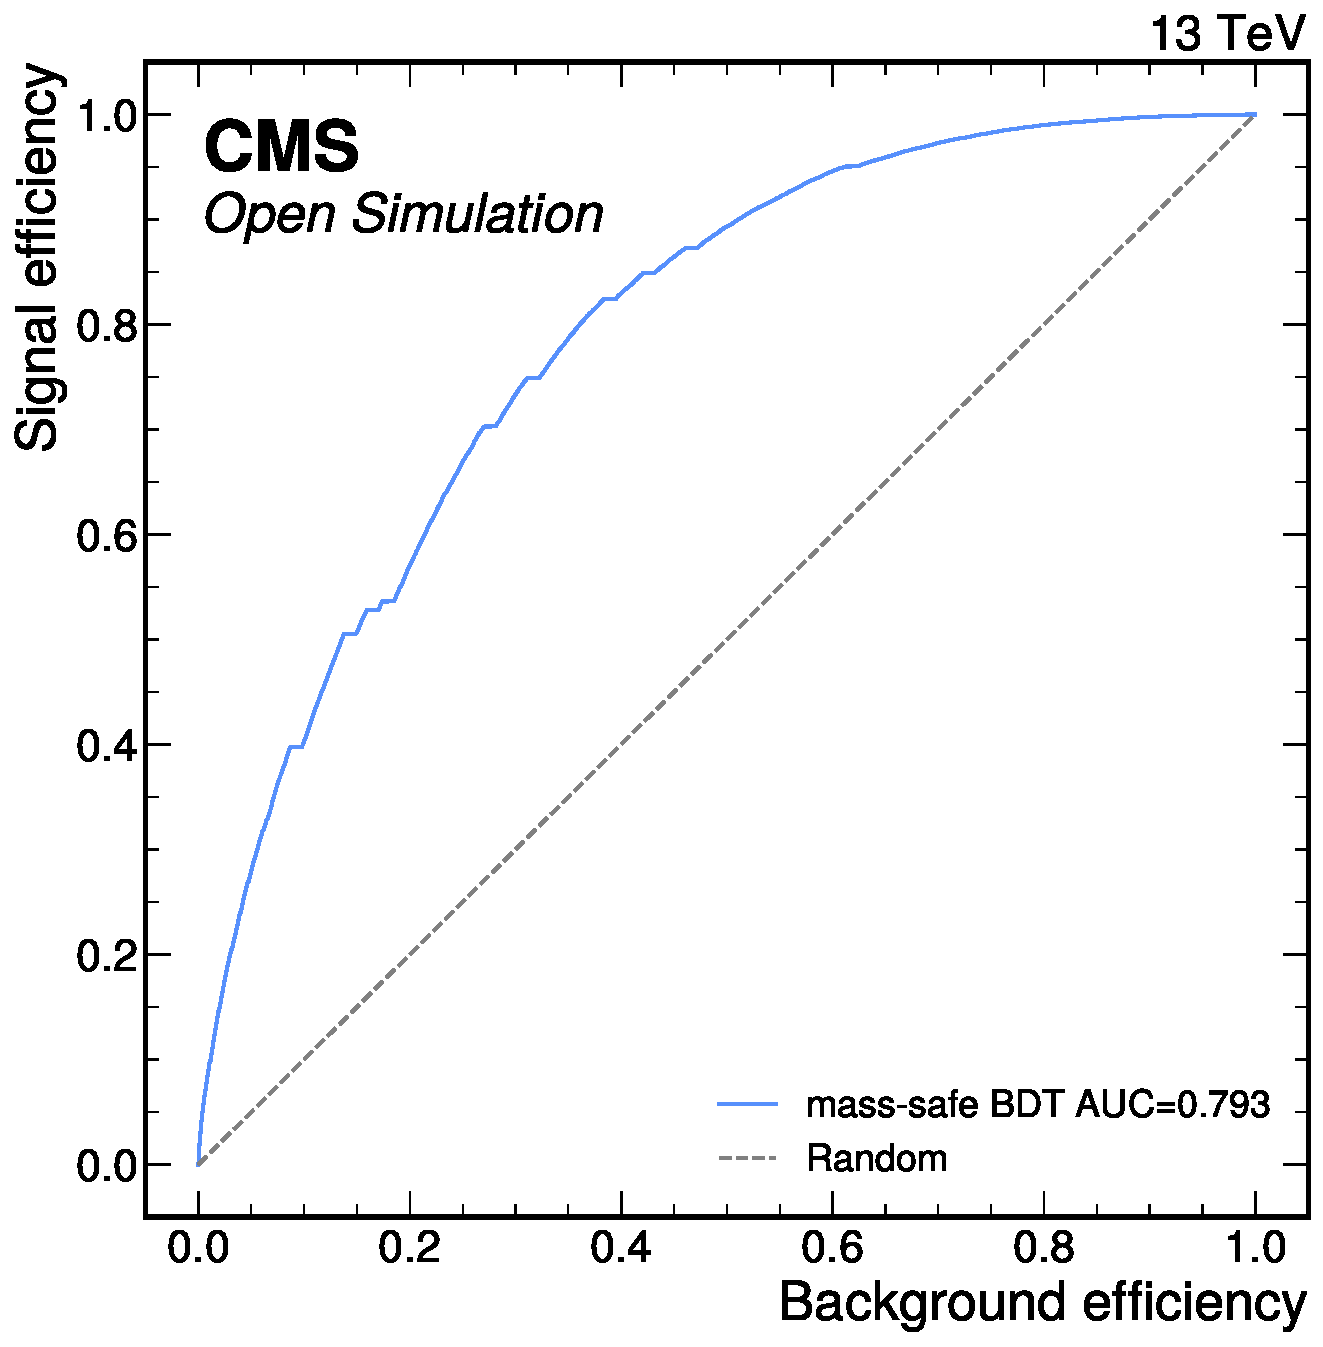
\includegraphics[width=0.92\linewidth,height=0.70\textheight,keepaspectratio]{figures/mva_roc_bdt_mass_safe.pdf}
\caption{Repaired mass-safe BDT ROC curve for the S2 attempt. The model is trained and evaluated in the broad $80<m_{4\ell}<170$ GeV MVA window while excluding $m_{4\ell}$ from the inputs, and it reaches AUC 0.7929. It is the best repaired classifier, but S2 is not promoted because score-shape, category viability, and mass-sculpting gates fail.}
\label{fig:mva-roc-bdt-mass-safe}
\end{figure}

\begin{figure}[p]
\centering
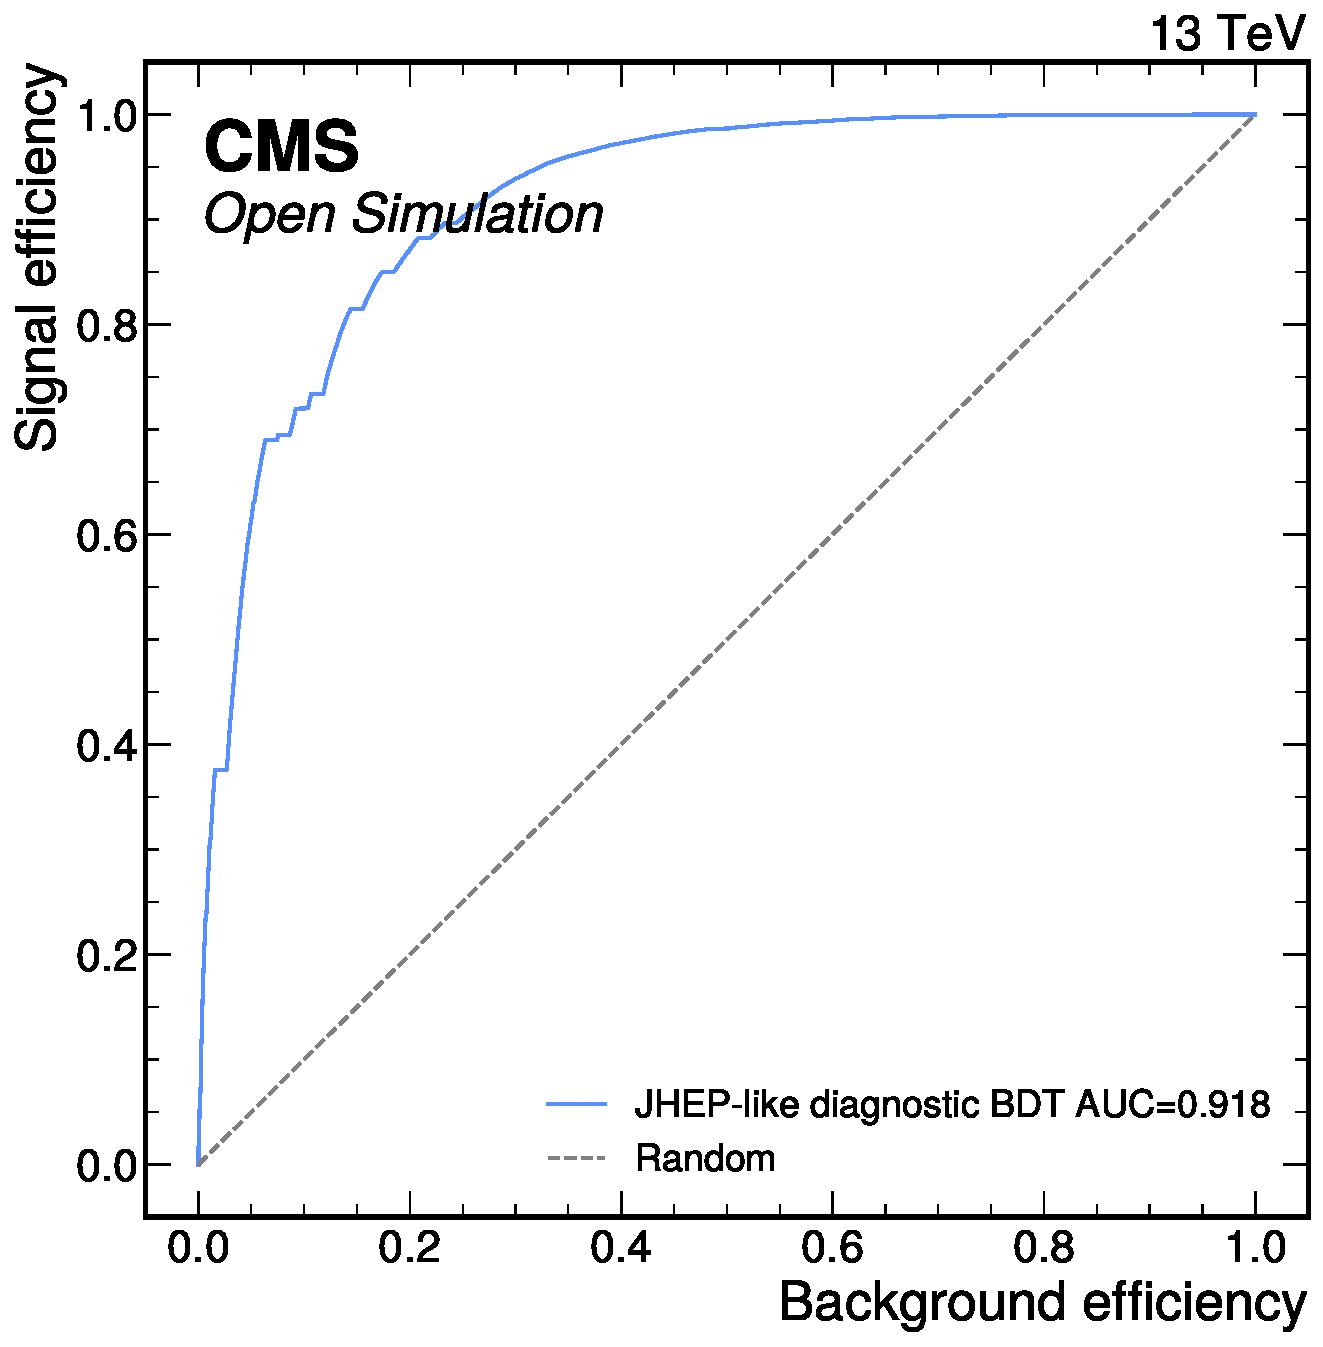
\includegraphics[width=0.92\linewidth,height=0.70\textheight,keepaspectratio]{figures/mva_roc_bdt_jhep_like_diagnostic.pdf}
\caption{JHEP-like diagnostic BDT ROC curve for the S2 attempt. This diagnostic reaches AUC 0.9176 because it includes mass-like variables such as $m_{Z1}$ and $m_{Z2}$, so it is not used to define nominal categories for the mass-spectrum fit.}
\label{fig:mva-roc-bdt-jhep-like-diagnostic}
\end{figure}

\begin{figure}[p]
\centering
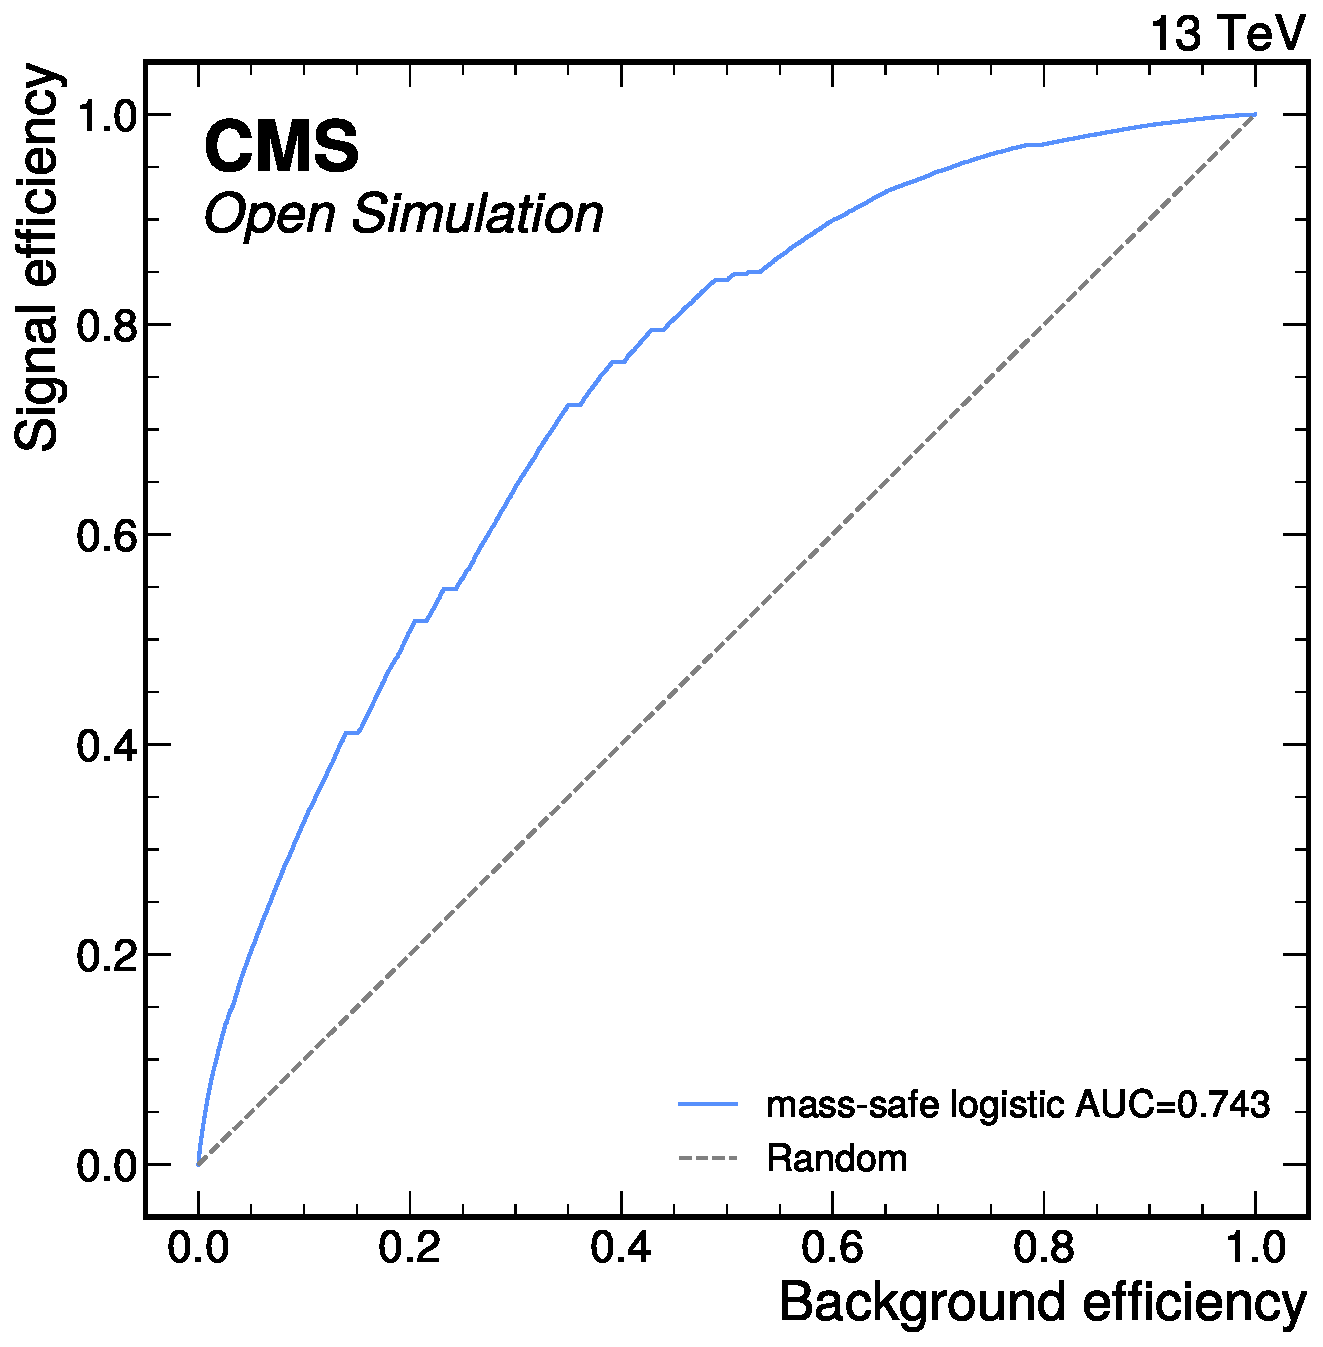
\includegraphics[width=0.92\linewidth,height=0.70\textheight,keepaspectratio]{figures/mva_roc_logistic_mass_safe.pdf}
\caption{Repaired mass-safe logistic ROC curve for the S2 attempt. The logistic baseline reaches AUC 0.7430 in the broad training window and is retained as a transparent cross-check of the BDT separation. No classifier category enters the nominal likelihood.}
\label{fig:mva-roc-logistic-mass-safe}
\end{figure}

\begin{figure}[p]
\centering
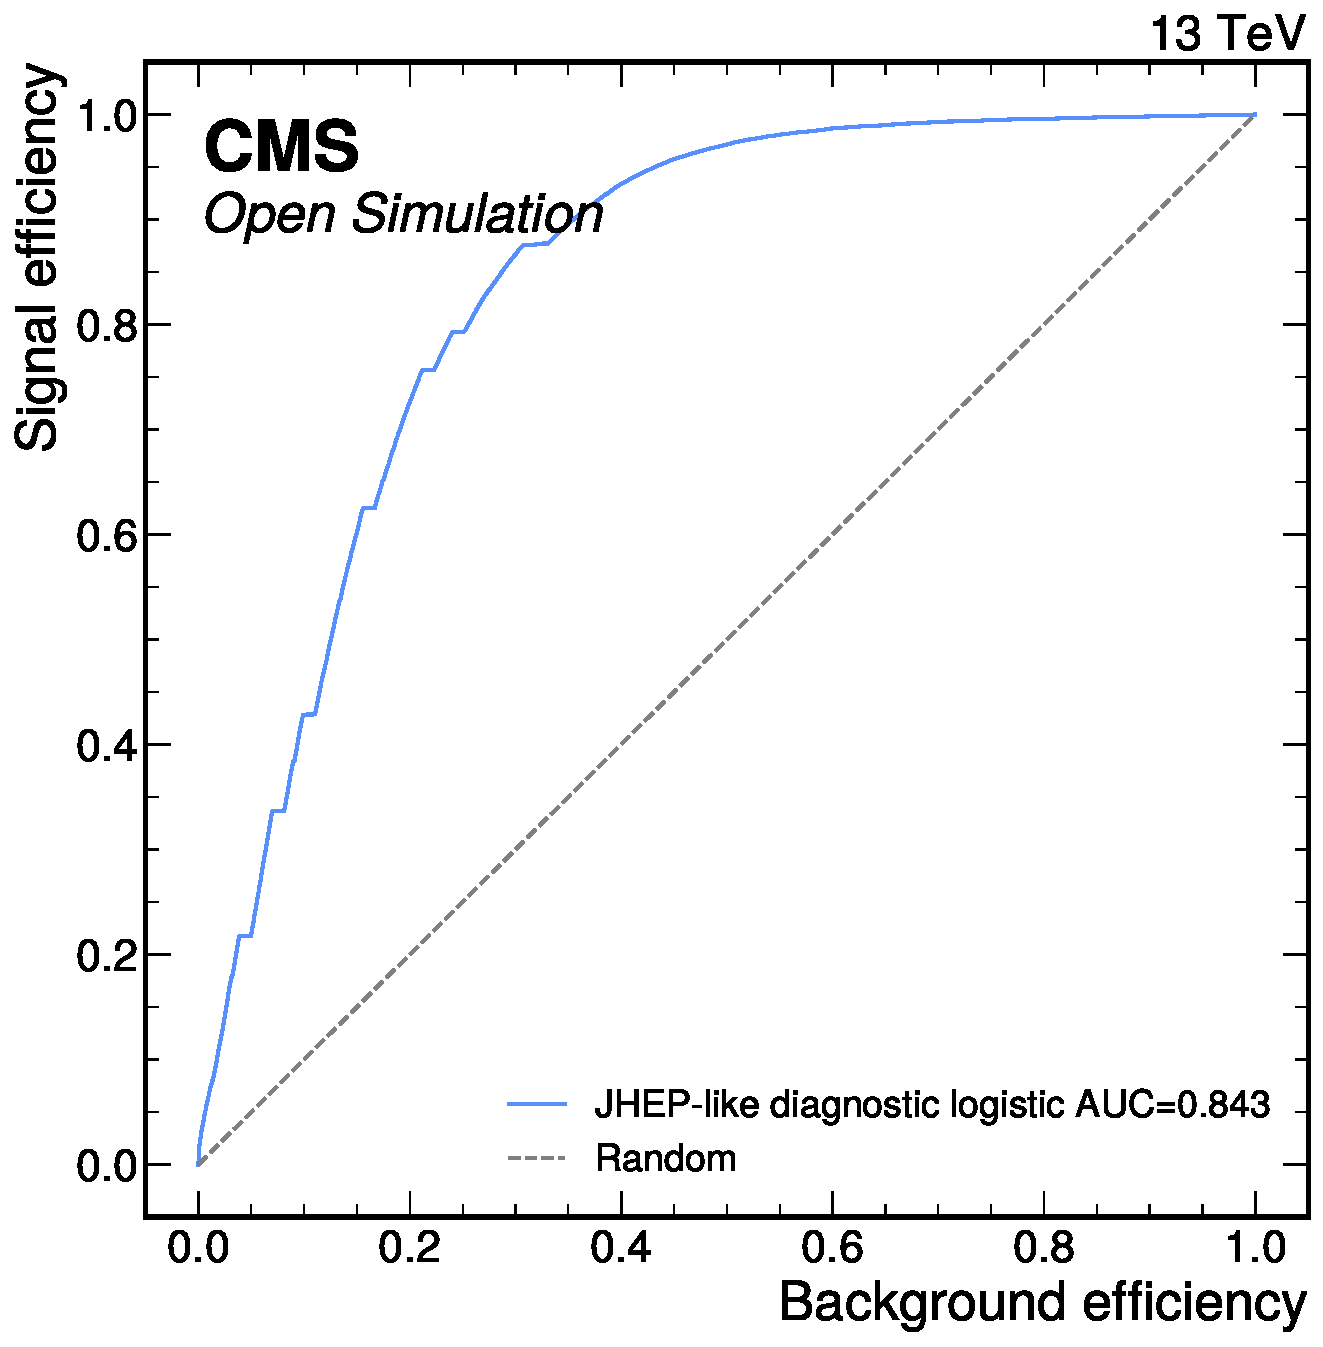
\includegraphics[width=0.92\linewidth,height=0.70\textheight,keepaspectratio]{figures/mva_roc_logistic_jhep_like_diagnostic.pdf}
\caption{JHEP-like diagnostic logistic ROC curve for the S2 attempt. This diagnostic reaches AUC 0.8428 with mass-like inputs and is shown only to document why the safer classifier definition is used for promotion decisions.}
\label{fig:mva-roc-logistic-jhep-like-diagnostic}
\end{figure}

\begin{figure}[p]
\centering
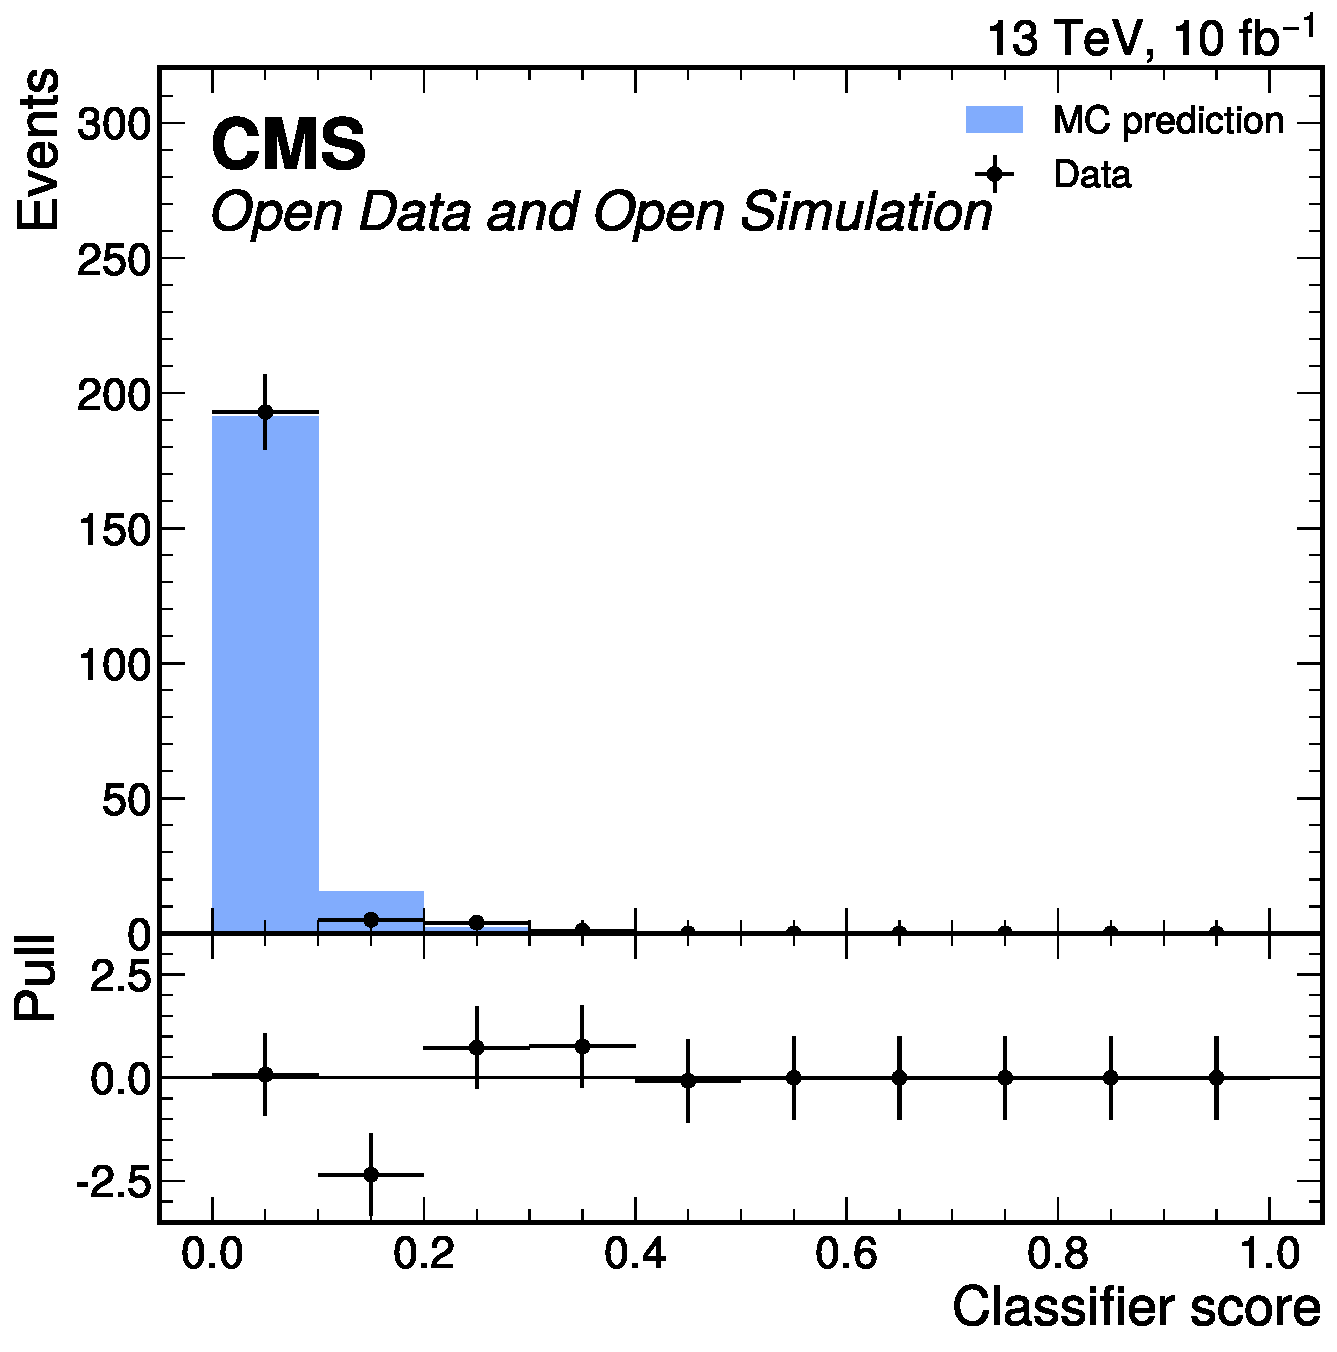
\includegraphics[width=0.92\linewidth,height=0.70\textheight,keepaspectratio]{figures/mva_best_score_datamc.pdf}
\caption{Best repaired MVA score data/MC comparison. The best mass-safe BDT has a 19.0\% precision-proxy improvement relative to S1, but the score-shape validation fails and the promotion decision remains \texttt{promote\_s2=false}.}
\label{fig:mva-best-score-datamc}
\end{figure}


\section{Limitation Index}
\begin{small}
\begin{longtable}{p{0.14\linewidth}p{0.23\linewidth}p{0.55\linewidth}}
\caption{Constraint, decision, and limitation index carried into Doc 4a.}\label{tab:limitation-index}\\
\toprule
Label & Status & Impact \\
\midrule
\endfirsthead
\toprule
Label & Status & Impact \\
\midrule
\endhead
A1/D1 & Resolved & Primary prompt paths used; local copies not mixed. \\
A2/SP2 & Implemented fallback & Prompt cross sections used with process nuisances. \\
A3/D4 & Formally downscoped & No VBF category or jet systematics. \\
A4/D8 & Resolved for attempt & Angular variables recomputed and validated before NN attempt. \\
A5 & Limitation & No truth-level object closure claims. \\
A6/SP6 & Documented not propagated & PV variables excluded; no PV nuisance in nominal fit. \\
L1 & Active limitation & Detector-level open-data analysis, not official CMS calibration. \\
L2/SP10 & Active limitation & DY+jets MC fake proxy replaces data-driven Z+X. \\
L3/D9 & Active limitation & Mass scan is closure evidence, not official mass measurement. \\
SP3 & Formal downscope & Grouped MC-stat approximation replaces full bin-by-bin staterror. \\
VT12 & Passed with caveat & Mass-template injected closure passes; result not promoted to official measurement. \\
Corruption -20\% & Documented infeasible & Three final-state-aligned tests do not reject in low-count workspace. \\
\bottomrule
\end{longtable}
\end{small}
\section{Reproduction Contract}
A fresh analyst should reproduce the current expected, partial-data, and full-data results with the following commands from the analysis root:
\begin{enumerate}[leftmargin=*]
\item \texttt{pixi install} to materialize the analysis environment.
\item \texttt{pixi run all} to run the chain through the current task definition.
\item \texttt{pixi run p3-all} to rebuild selection tables, VBF downscope evidence, angular closure, input validation, MVA diagnostics, and selection figures.
\item \texttt{pixi run p4a-all} to rebuild the expected pyhf workspace outputs, result JSON files, figures, and commitments.
\item \texttt{pixi run p4b-all} or the current Phase 4b task sequence to rebuild the fixed-seed 10\% observed-data JSON and figures.
\item \texttt{pixi run p4c-all} to rebuild the full observed-data JSON and figures, preserving the active $70 < m_{4\ell} < 170$ GeV fit window.
\item From \texttt{analysis\_note/}, run \texttt{tectonic ANALYSIS\_NOTE\_doc4c\_v1.tex} to compile this note.
\end{enumerate}
The execution DAG is: prompt and ROOT ntuples $\rightarrow$ Phase 1 metadata/literature inventory $\rightarrow$ Phase 2 strategy commitments $\rightarrow$ Phase 3 selection and categories $\rightarrow$ Phase 4a expected workspace/results JSON $\rightarrow$ Phase 4b fixed-seed 10\% observed-data workspace/results JSON $\rightarrow$ Phase 4c full observed-data workspace/results JSON $\rightarrow$ Doc 4c LaTeX/PDF. Manual steps are limited to writing this note, staging figures, and reviewing rendered output.
\section{Machine-Readable Result Files}
The numerical source of truth for Doc 4c is the JSON collection in the results directory. It contains expected, partial, and observed parameters, covariance, validation, mass scan, systematic summary, systematic shifts, and systematic-source records. The final observed-data files are:
\begin{itemize}[leftmargin=*]
\item observed\_parameters.json and observed\_validation.json,
\item observed\_covariance.json and observed\_systematics.json,
\item observed\_mass\_scan.json and observed\_systematic\_shifts.json,
\item expected\_* and partial\_* JSON files for baseline and validation cross-checks.
\end{itemize}
Upstream selection JSON provides normalization, cutflow, input-validation, MVA metadata, approach-comparison, and selected-configuration records.
\clearpage
\bibliographystyle{unsrt}
\bibliography{../references}
\end{document}
